\documentclass[UTF8]{ctexart}
% shumo.sty 包含完整文档导致加载错误，改为按需加载宏包
% \usepackage{shumo}
\usepackage{geometry}
\usepackage{listings}
\usepackage{xcolor}
\usepackage{float}
\usepackage{booktabs}
\usepackage{amsmath,amssymb}
\usepackage{graphicx}
\usepackage{tabularx}
\usepackage{fancyhdr}
% shumo.sty 中定义的字号与字体命令在此简化定义以保持兼容
\providecommand{\sihao}{}
\providecommand{\xiaosihao}{}
\providecommand{\heiti}{\textbf}
\title{\textbf{考虑风场影响的民用客机高度--速度联合巡航优化模型}}% 请勿修改
\date{}%请勿添加自己的信息
\author{}%请勿添加自己的信息
%下面时正文
\begin{document}
\setcounter{page}{1}%从正文开始计算页码	
\maketitle
\vspace{-0.95cm}
\thispagestyle{fancy}   
\fancyhf{} %清除原本页眉页脚形式
\renewcommand{\headrulewidth}{0pt} %页眉线宽，设为0可以去页眉线
%=================================================
%=================================================
%=================================================
%=================================================
%=================================================
%=================================================
%下面开始出现各位需要修改的部分。
\renewcommand{\abstractname}{\sihao 摘\quad 要} %更改摘要二字的样式
\begin{abstract}
随着航空燃油价格波动、碳排放约束增强以及航空公司运行成本压力上升，如何通过科学的巡航策略降低燃油消耗，已成为民用客机运行优化中的重要问题。针对某型民用客机巡航飞行的高度--速度联合优化问题，本文以\textbf{燃油消耗最小化}和\textbf{巡航策略优化}为核心目标，建立了从动力学建模、路径油耗积分、最优控制求解到综合数值分析的完整模型框架。

针对问题一，本文依据气动力平衡、推力--阻力平衡和质量守恒关系，建立了以飞行距离和飞机质量为状态变量、以飞行高度和空速为控制变量的巡航动力学模型。模型中综合考虑了升力、阻力等之间的耦合关系，并在燃油消耗率中引入速度偏离最佳经济速度的惩罚项。进一步地，本文分别推导了\textbf{等速巡航爬升策略}和\textbf{等马赫数巡航爬升策略}下高度随质量和时间变化的演化规律。数值结果表明，在给定初始质量 $72450\ \mathrm{kg}$、终止质量 $62000\ \mathrm{kg}$ 的条件下，两种策略总燃油消耗均为 $10450\ \mathrm{kg}$；等速策略最终高度为 $10637.1\ \mathrm{m}$，总飞行时间为 $12.7076\ \mathrm{min}$；等马赫数策略最终高度为 $10437.8\ \mathrm{m}$，总飞行时间为 $13.5265\ \mathrm{min}$。

针对问题二，本文在问题一动力学模型基础上，建立了总燃油消耗的\textbf{路径积分模型}。通过将时间域油耗率转化为单位航程油耗率，明确了大气密度、温度、声速和风场随高度变化对燃油消耗的作用路径。数值计算表明，标准大气条件下，等速策略平均单位航程油耗率为 $0.052039\ \mathrm{kg/m}$，等马赫数策略为 $0.049414\ \mathrm{kg/m}$。进一步考虑恒定 $5\ \mathrm{K}$ 温度偏差和线性温度偏差后，两种策略总油耗变化均约为 $0.1\%$，表明在温度偏差主要改变局部气动参数和声速，对总油耗影响较小。

针对问题三，本文将高度和速度同时纳入状态变量，引入高度变化率和速度变化率作为控制变量，建立了以总燃油消耗最小为目标的\textbf{高度--速度联合最优控制模型}。模型同时考虑高度范围、速度范围等约束，并通过哈密顿函数给出了最优轨迹应满足的必要条件。由于模型具有较强非线性，本文采用时间域梯形配点法将连续最优控制问题转化为非线性规划问题，并利用 SLSQP 算法求解。结果显示，在固定航程条件下，无风最优轨迹总油耗为 $8947.394\ \mathrm{kg}$，有风最优轨迹总油耗为 $7707.451\ \mathrm{kg}$，相较无风情形节油约 $13.86\%$，飞行时间由 $777.724\ \mathrm{s}$ 缩短至 $660.884\ \mathrm{s}$。

针对问题四，本文进一步构建了完整的巡航策略综合数值计算模型，对等速基准策略、考虑风场的高度--速度联合最优策略及模型扩展进行了统一分析。在终止质量 $m_f=62000\ \mathrm{kg}$ 下，等速巡航基准策略航程为 $200809.924516\ \mathrm{m}$，总燃油消耗为 $10450\ \mathrm{kg}$；在固定相同航程条件下，考虑风场的联合最优策略总油耗降至 $8394.401214\ \mathrm{kg}$，节油比例达到 \textbf{$19.670802\%$}。最后，本文从\textbf{温度偏差实时修正}和\textbf{发动机安装损失}两个方向进行模型扩展。结果表明，温度修正通过改变真实密度和声速影响气动与马赫数约束，发动机安装损失则通过放大指令推力提高燃油消耗率；二者均未改变原有动力学主框架，但引入了新的非线性耦合关系，使模型更加贴近实际飞行工程场景。
\end{abstract}

\noindent\textbf{关键词：} 高度--速度联合优化；燃油消耗模型；最优控制；垂直风切变；路径积分

\pagestyle{plain}
%标准 LaTeX 提供下列四种页版式，可用 \pagestyle{页版式} 命令来设置页面版式：
%empty(没有页眉和页脚)，plain(本次用的，无页眉，页脚为居中页码)，headings(页眉为章节标题，无页脚)，myheadings(页眉内容可自定义，无页脚)
\newpage

\section{问题重述}
\subsection{问题背景}
在全球航空燃油价格波动、碳排放约束以及航空公司运营成本压力不断增大的背景下，如何通过科学的巡航策略降低燃油消耗，已成为飞行运行管理和飞机性能优化中的重要问题。
\begin{figure}[H]
	\centering
	\IfFileExists{1.png}{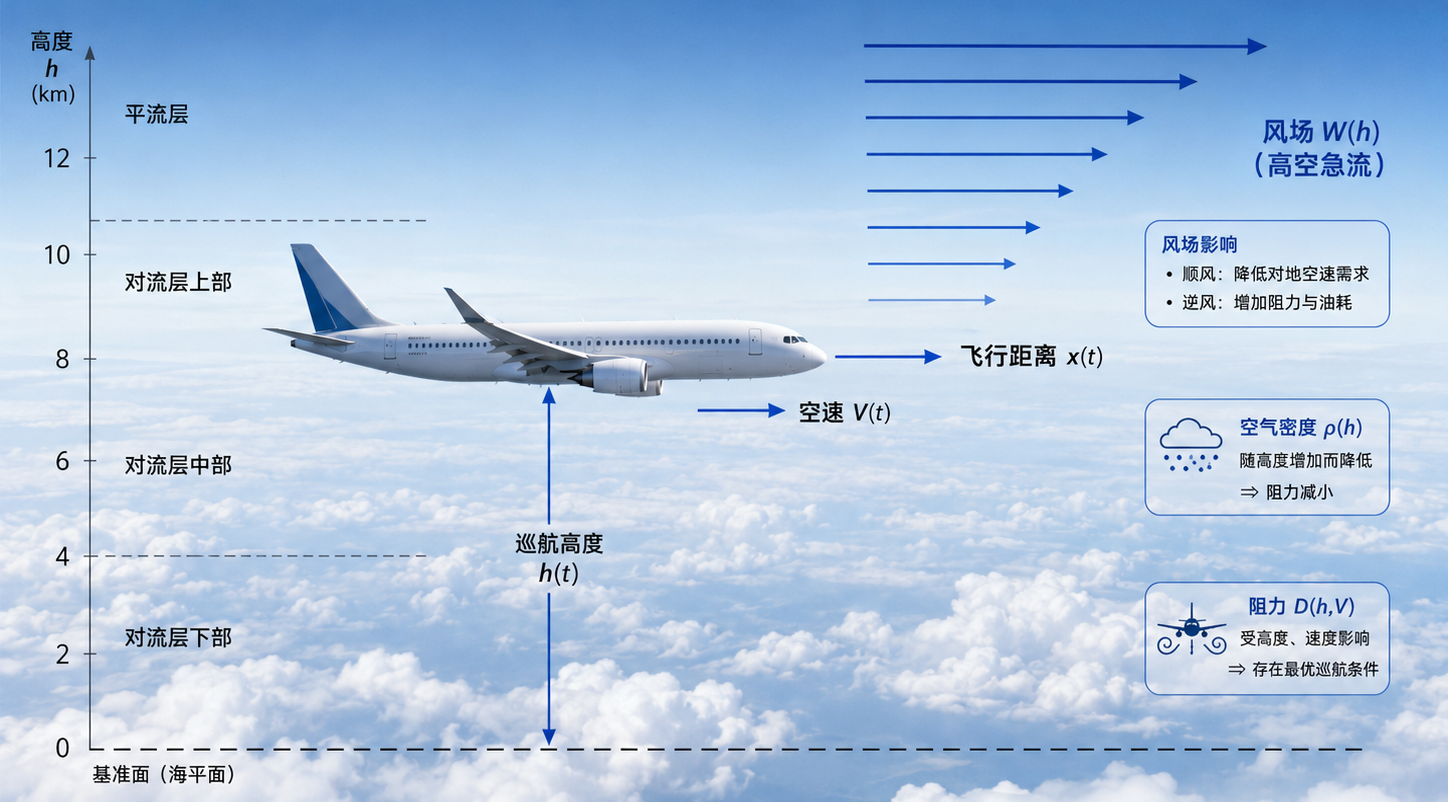
\includegraphics[width=0.65\textwidth]{1.png}}{\fbox{Missing figure}}
	\caption{飞机飞行状态示意图}
	\label{fig:pipe1_comparison}
\end{figure}
\subsection{问题提出}
基于题目给定的飞机参数、初始状态和终止质量条件，本文需要依次解决以下问题。

\textbf{问题一}：根据气动力平衡和能量守恒原理，建立飞机巡航过程中水平位移、飞机质量、高度和空速之间的耦合动力学模型。并进一步推导等速巡航爬升策略和等马赫数巡航爬升策略下的高度演化规律，比较两种策略的高度剖面、质量剖面、爬升率、总飞行时间和燃油消耗量。

\textbf{问题二}：建立沿飞行路径积分的总燃油消耗模型，明确标准大气中温度、密度和声速随高度连续变化对油耗模型的影响。进一步考虑实际大气温度偏差，选择合理的修正方法，建立修正后的油耗率模型，并分析温度偏差对总油耗计算结果和系统非线性结构的影响。

\textbf{问题三}：在给定初始飞行状态下，以总燃油消耗最小为目标，建立高度--速度联合最优巡航控制模型。并通过合适的最优控制方法推导最优轨迹满足的必要条件，比较无风与有垂直风切变条件下最优解结构的变化。

\textbf{问题四}：在前三问基础上，建立完整的巡航策略综合数值计算模型。定量比较等速巡航爬升策略和考虑风场条件下的高度--速度联合轨迹两者燃油消耗、航程变化和节油比例；同时分析速度偏离惩罚系数变化对最优轨迹的影响，并从温度偏差修正、小角度非水平爬升、发动机安装损失、多机协同与空域约束等方向中选择至少两个进行模型扩展。

\section{问题分析}

\subsection{问题一的分析}
问题一要求建立飞机巡航阶段的动力学模型，并分析等速巡航爬升和等马赫数巡航爬升两种典型策略。巡航过程中，飞机质量因燃油消耗不断减小，而高度、空速、大气密度及气动力之间又存在较强耦合关系，因此首先需要依据飞行动力学原理建立巡航过程的数学模型。随后，在不同控制策略下对模型进行适当简化，分别推导两种巡航方式的高度变化规律，并结合题目给定参数进行数值计算，对比两种策略在爬升率、飞行时间及燃油消耗等方面的差异，为后续优化提供基础模型。

\subsection{问题二的分析}
问题二在问题一动力学模型的基础上，进一步关注巡航全过程的燃油消耗计算。由于飞机飞行过程中所处的大气环境随高度连续变化，大气密度、温度和声速均会影响气动力及发动机效率，因此需要建立能够反映大气参数变化影响的燃油消耗模型。同时，针对实际飞行中可能出现的温度偏差，需要建立修正模型，并通过数值计算分析温度修正对燃油消耗结果的影响程度，从而判断不同大气条件下模型的适用范围及修正的必要性。

\subsection{问题三的分析}
问题三要求在满足飞行动力学约束、升力平衡及飞行包线限制的条件下，以总燃油消耗最小为目标，建立高度与速度联合优化模型。由于控制变量与状态变量之间存在明显的非线性耦合关系，该问题本质上属于连续最优控制问题。建模过程中需要综合考虑高度变化、速度调整及风场影响对燃油消耗的共同作用，并选择合适的优化方法进行求解。同时，通过比较无风和有风条件下最优轨迹的变化规律，分析风场对最优巡航策略的影响，并评价不同求解方法在复杂约束条件下的适用性。

\subsection{问题四的分析}
问题四是在前三问基础上的综合应用与模型扩展。首先，需要建立完整的数值计算流程，对等速巡航策略和最优巡航策略进行统一计算与比较，分析最优策略在燃油节省、飞行时间及航程等方面的优势。随后，通过改变模型参数分析最优轨迹对参数扰动的敏感性，识别影响巡航性能的关键因素。最后，结合实际飞行环境，从温度偏差、小角度非水平飞行、发动机安装损失、多机协同等方面对模型进行扩展，使模型更加符合实际工程应用，提高模型的通用性和实际参考价值。


\section{模型假设与符号说明}

\subsection{模型假设}
\begin{enumerate}
    \item 飞机巡航阶段可视为小角度爬升过程，航迹角较小，故有 $\cos\gamma\approx 1$；
    \item 飞机在巡航过程中保持准定常飞行状态，升力近似平衡飞机重量；
    \item 除燃油消耗外，飞机其他载荷质量保持不变，因此飞机质量变化仅由燃油消耗引起；
    \item 风场仅影响飞机相对于地面的水平速度，不改变飞机相对于空气的空速；
    \item 在基准模型中，采用指数大气模型描述大气密度随高度的变化。
\end{enumerate}

\subsection{符号说明}
\begin{table}[htbp]
\centering
\caption{主要符号说明}
\label{tab:symbols}
\begin{tabular}{ccl}
\toprule
符号 & 说明 & 单位 \\
\midrule
$x(t)$ & 飞机相对于地面的累计飞行距离& \\
$m(t)$ & 飞机实时总质量（含剩余燃油& \\
$h(t)$ & 飞机巡航高度& \\
$V(t)$ & 飞机空速& \\
$M(t)$  & 飞机马赫数& -- \\
$F(t)$ & 发动机推力 & N \\
$D(t)$  & 飞机气动阻力& N \\
$\dot m_f(t)$  & 燃油消耗率& kg/s \\
$C_L(t)$ & 升力系数& -- \\
$\rho(h(t))$ & 高度 $h(t)$ 处的大气密度& kg/m³ \\
$a(h)$& 高度 $h$ 处的声速& m/s \\
$W(h)$& 高度 $h$ 处的水场风速& m/s \\
$q(x)$ & 单位航程燃油消耗率& kg/m \\
$J$ & 总燃油消耗量& kg \\
\bottomrule
\end{tabular}
\end{table}
\section{模型准备}
\subsection{燃油消耗率}
根据推力燃油消耗率（TSFC）的定义，单位时间内的燃油消耗量与发动机推力需求近似成正比，由此可建立基础燃油消耗率模型：
\begin{equation}
    \dot{m}_f(t)=c_f F(t),
\end{equation}
其中，$c_f$ 表示推力燃油消耗系数，$F(t)$ 表示发动机在 $t$ 时刻的推力需求。

在实际巡航过程中，发动机燃油效率除受推力影响外，还与飞行速度密切相关。研究表明，巡航速度的选择会显著改变燃油消耗，且存在使油耗最低的经济巡航速度，该最优速度通常取决于飞行高度、飞机质量、航程及运行成本等因素\cite{1}。为刻画这一特性，本文在基础模型上引入速度偏离惩罚项，用以描述空速$V(t)$偏离经济速度$V_{\mathrm{opt}}$时所产生的额外油耗：
\begin{equation}
    \dot{m}_f(t)
    =
    c_f F(t)
    \left[
    1+\beta\left(V(t)-V_{\mathrm{opt}}\right)^2
    \right],
\end{equation}
其中，$V_{\mathrm{opt}}$ 表示参考最佳经济巡航速度，$\beta$ 表示速度偏离惩罚系数。

\subsection{大气密度}
巡航高度变化时，大气密度随之改变，进而影响飞机的升力、阻力及推力需求。根据标准大气特性，本文采用指数衰减模型\cite{2}描述密度随高度的变化：
\begin{equation}
    \rho(h)=\rho_0 e^{-h/H_\rho} ,
\end{equation}
其中，$\rho_0$ 表示海平面大气密度，$H_\rho$ 表示大气标高。
\subsection{马赫数与声速}
声速依赖于大气温度，采用国际标准大气的线性温度模型：
\begin{equation}
    T(h)=T_0-L_T h,
    \label{eq:T_model}
\end{equation}
其中，$T_0$ 为海平面标准温度，$L_T$ 为温度递减率。由此声速可表示为：
\begin{equation}
    a(h)=\sqrt{\gamma R_{\mathrm{gas}}T(h)}.
    \label{eq:sound_speed_model}
\end{equation}
其中$\gamma$表示空气的比热比，$R_{\mathrm{gas}}$表示气体常数，则马赫数可表示为：
\begin{equation}
    M(t)=\frac{V(t)}{a(h(t))}.
    \label{eq:mach_model}
\end{equation}
\subsection{风场}
题目给定的风场仅依赖于飞行高度，其表达式为：
\begin{equation}
    W(h)=20+0.00003(h-10000)^2.
    \label{eq:wind_model}
\end{equation}

\section{问题一模型建立与求解}
\subsection{模型建立}
\subsubsection{升力模型}

对于巡航阶段的固定翼飞机，其升力可由动压、机翼面积和升力系数共同表示为\cite{5}
\begin{equation}
    L(t)=\frac{1}{2}\rho(h(t))V^2(t)S C_L(t),
    \label{eq:lift}
\end{equation}
其中，$\rho(h(t))$ 表示高度 $h(t)$ 处的大气密度，$V(t)$ 表示飞机空速，
$S$ 表示机翼面积，$C_L(t)$ 表示升力系数。

在小角度巡航爬升近似下，飞机垂直方向近似满足升力与重力平衡，即
\begin{equation}
    L(t)=m(t)g.
    \label{eq:lift_balance}
\end{equation}
由式 (4) 和式 (5) 可得升力系数为
\begin{equation}
    C_L(t)=\frac{2m(t)g}{\rho(h(t))V^2(t)S}.
    \label{eq:CL}
\end{equation}
\subsubsection{阻力模型}

飞机巡航过程中的总阻力可表示为\cite{6}
\begin{equation}
    D(t)=\frac{1}{2}\rho(h(t))V^2(t)S C_D(t),
    \label{eq:drag}
\end{equation}
其中，$C_D(t)$ 表示总阻力系数。本文采用经典抛物线阻力极曲线描述阻力系数\cite{3}，
即
\begin{equation}
    C_D(t)=C_{D0}+kC_L^2(t),
    \label{eq:CD}
\end{equation}
其中，$C_{D0}$ 表示零升阻力系数，$k$ 表示升致阻力因子。$C_{L}$ 表示升力系数

将式 (12) 代入式 (11)，可将总阻力分解为零升阻力和升致阻力：
\begin{equation}
    D(t)=D_0(t)+D_i(t),
    \label{eq:D_decompose}
\end{equation}
其中
\begin{equation}
    D_0(t)=\frac{1}{2}\rho(h(t))V^2(t)S C_{D0},
    \qquad
    D_i(t)=\frac{1}{2}\rho(h(t))V^2(t)S kC_L^2(t).
    \label{eq:D0_Di}
\end{equation}
零升阻力主要与机体外形、飞行速度和大气密度有关；升致阻力则来源于飞机产生升力的过程，
其大小与升力系数的平方成正比。\cite{7}

\subsubsection{推力需求模型}
在飞机航迹方向上，根据牛顿第二定律，可得到
\begin{equation}
    m(t)\dot V(t)
    =
    F(t)-D(t)-m(t)g\sin\gamma,
    \label{eq:force_balance}
\end{equation}
其中，$\dot V(t)$ 表示空速变化率，$F(t)$ 表示发动机推力，$D(t)$ 表示巡航阻力，$\gamma$ 表示航迹角。

高度变化率与航迹角之间满足
\begin{equation}
    \dot h(t)=V(t)\sin\gamma.
    \label{eq:h_dot}
\end{equation}
将式 (16) 代入式 (15)，并整理可得发动机推力需求模型：
\begin{equation}
    F(t)=D(t)+m(t)\dot V(t)
    +\frac{m(t)g}{V(t)}\dot h(t).
    \label{eq:thrust}
\end{equation}
\subsubsection{燃油消耗与质量变化模型}
飞机巡航过程中，发动机推力输出会持续消耗燃油。根据推力燃油消耗率模型，
单位时间燃油消耗率可表示为
\begin{equation}
    \dot m_f(t)
    =
    c_fF(t)
    \left[
    1+\beta\left(V(t)-V_{\mathrm{opt}}\right)^2
    \right],
    \label{eq:fuel_rate}
\end{equation}
其中，$c_f$ 表示推力燃油消耗系数，$V_{\mathrm{opt}}$ 表示参考最佳经济巡航速度，
$\beta$ 表示速度偏离惩罚系数。

由于巡航过程中除燃油外的其他载荷可近似认为保持不变，飞机总质量变化主要由燃油消耗引起，
因此质量变化方程为
\begin{equation}
    \dot m(t)=-\dot m_f(t).
    \label{eq:mass_change}
\end{equation}
将式 (18)带入质量变化方程，可得
\begin{equation}
    \dot m(t)
    =
    -c_fF(t)
    \left[
    1+\beta\left(V(t)-V_{\mathrm{opt}}\right)^2
    \right].
    \label{eq:mass_ode}
\end{equation}

\subsubsection{水平运动方程}

风场只改变飞机相对于地面的水平速度，不改变飞机相对于空气的空速。
在小角度巡航近似下，飞机水平地速可表示为空速与高度相关风速的叠加，
因此水平运动方程为\cite{8}
\begin{equation}
    \dot x(t)=V(t)+W(h(t)),
    \label{eq:x_ode}
\end{equation}
其中，$W(h(t))$ 表示高度 $h(t)$ 处的水平风速。

\subsubsection{综合状态方程组}

综上，飞机巡航过程可描述为由飞行距离和飞机质量构成的状态方程组：
\begin{equation}
\left\{
\begin{aligned}
    \dot x(t) &= V(t)+W(h(t)),\\
    \dot m(t) &=
    -c_fF(t)
    \left[
    1+\beta\left(V(t)-V_{\mathrm{opt}}\right)^2
    \right],
\end{aligned}
\right.
\label{eq:state_system}
\end{equation}
\subsubsection{等速巡航爬升与等马赫数巡航爬升的高度演化规律}
在巡航爬升过程中，飞机通常希望保持在较优气动效率附近飞行。为此，本文假设飞机在两种基准巡航爬升策略下均保持参考经济升力系数 $C_{L,c}$ 不变。该参考升力系数由初始状态确定：
\begin{equation}
    C_{L,c}
    =
    \frac{2m_0g}{\rho(h_0)V_0^2S}.
    \label{eq:CLc}
\end{equation}

根据升力平衡条件，有
\begin{equation}
    \frac{1}{2}\rho(h(t))V^2(t)S C_{L,c}
    =
    m(t)g.
    \label{eq:lift_balance_cruise_climb}
\end{equation}

由上式可知，在保持升力系数近似不变的条件下，
飞机质量、飞行高度和空速之间存在确定的代数关系。随着燃油消耗导致飞机质量下降，
飞机需要通过调整高度或速度来维持升力平衡。

\paragraph{等速巡航爬升策略}

等速巡航爬升策略是指飞机在巡航爬升过程中保持空速不变，即
\begin{equation}
    V(t)=V_c,
    \qquad
    \dot V(t)=0.
    \label{eq:constant_speed_condition}
\end{equation}

其中，$V_c$ 可取初始空速 $V_0$。将式（25）
代入升力平衡式 （28），可得
\begin{equation}
    \rho(h(t))
    =
    \frac{2m(t)g}{V_c^2S C_{L,c}}.
    \label{eq:rho_constant_speed}
\end{equation}

其中$\rho(h(t)$可由指数大气模型表示
\begin{equation}
	\rho(h)=\rho_0 e^{-h/H_\rho} ,
    \label{eq:rho_exp_for_climb}
\end{equation}

将两式联立则有
\begin{equation}
    \rho_0 e^{-h(t)/H_\rho} 
    =
    \frac{2m(t)g}{V_c^2S C_{L,c}}.
    \label{eq:constant_speed_h_m}
\end{equation}

由初始时刻同样满足升力平衡，可将式 (28) 写成相对形式：
\begin{equation}
    \frac{m(t)}{m_0}
    = e^{-\frac{h(t)-h_0}{H_\rho}}.
    \label{eq:constant_speed_relative}
\end{equation}

于是，等速巡航爬升策略下高度关于质量的演化规律为
\begin{equation}
    h(t)
    =
    h_0
    -
    H_\rho
    \ln\frac{m(t)}{m_0}.
    \label{eq:constant_speed_h_t}
\end{equation}

对式 (30) 关于时间求导，得到等速巡航爬升率：
\begin{equation}
    \dot h(t)
    =
    -H_\rho\frac{\dot m(t)}{m(t)}.
    \label{eq:constant_speed_h_dot_1}
\end{equation}

由于飞机质量变化方程为
\begin{equation}
    \dot m(t)=-\dot m_f(t),
    \label{eq:m_dot_fuel}
\end{equation}
因此
\begin{equation}
    \dot h(t)
    =
    H_\rho
    \frac{\dot m_f(t)}{m(t)}.
    \label{eq:constant_speed_h_dot}
\end{equation}

上述式子表明，在等速巡航爬升策略下，飞机爬升率与单位质量燃油消耗率成正比。
随着燃油消耗，飞机质量逐渐减小，为保持相同空速和相同升力系数，飞机需要进入密度更低的高空区域，
因此高度随时间逐渐增加。

进一步地，在等速条件下，推力需求模型可化简为
\begin{equation}
    F_c(t)
    =
    D_c(t)
    +
    \frac{m(t)g}{V_c}\dot h(t),
    \label{eq:constant_speed_thrust}
\end{equation}
燃油消耗率为
\begin{equation}
    \dot m_f(t)
    =
    c_fF_c(t)
    \left[
    1+\beta\left(V_c-V_{\mathrm{opt}}\right)^2
    \right].
    \label{eq:constant_speed_fuel}
\end{equation}

\paragraph{等马赫数巡航爬升策略}

等马赫数巡航爬升策略指飞机在巡航爬升过程中保持马赫数不变，即：
\begin{equation}
    M(t)=M_c,
    \qquad
    V(t)=M_ca(h(t)).
    \label{eq:constant_mach_condition}
\end{equation}
其中，$M_c$ 可由初始状态确定：
\begin{equation}
    M_c=\frac{V_0}{a(h_0)}.
    \label{eq:Mc_initial}
\end{equation}
其中$a(h_0)$表示初始高度的声速。

将等马赫数条件 （36） 代入升力平衡式
（24），可得
\begin{equation}
    \frac{1}{2}
    \rho(h(t))
    M_c^2a^2(h(t))
    S C_{L,c}
    =
    m(t)g.
    \label{eq:constant_mach_lift_balance}
\end{equation}

结合模型准备中的大气密度和声速模型，可得
\begin{equation}
    m(t)
    =
    \frac{S C_{L,c}M_c^2}{2g}
    \rho_0 e^{-\frac{h(t)}{H_\rho}}
    \gamma R_{\mathrm{gas}}T(h(t)).
    \label{eq:constant_mach_m_h}
\end{equation}

由初始时刻的升力平衡关系，可将式 (37) 写成相对形式：
\begin{equation}
    \frac{m(t)}{m_0}
    =
    e^{-\frac{h(t)-h_0}{H_\rho}}
    \frac{T(h(t))}{T(h_0)}.
    \label{eq:constant_mach_relative}
\end{equation}
为了得到爬升率表达式，对式 (40) 两边取对数：
\begin{equation}
    \ln\frac{m(t)}{m_0}
    =
    -\frac{h(t)-h_0}{H_\rho}
    +
    \ln\frac{T(h(t))}{T(h_0)}.
    \label{eq:constant_mach_log}
\end{equation}

对时间求导，得到
\begin{equation}
    \frac{\dot m(t)}{m(t)}
    =
    -\frac{1}{H_\rho}\dot h(t)
    +
    \frac{T'(h(t))}{T(h(t))}\dot h(t).
    \label{eq:constant_mach_derivative}
\end{equation}

由于 $T'(h)=-L_T$，因此
\begin{equation}
    \frac{\dot m(t)}{m(t)}
    =
    -
    \left[
    \frac{1}{H_\rho}
    +
    \frac{L_T}{T(h(t))}
    \right]
    \dot h(t).
    \label{eq:constant_mach_mdot}
\end{equation}

结合质量变化方程 $\dot m(t)=-\dot m_f(t)$，可得等马赫数巡航爬升率：
\begin{equation}
    \dot h(t)
    =
    \frac{\dot m_f(t)}{m(t)}
    \left[
    \frac{1}{H_\rho}
    +
    \frac{L_T}{T(h(t))}
    \right]^{-1}.
    \label{eq:constant_mach_h_dot}
\end{equation}

式(44) 表明，等马赫数巡航爬升率不仅与单位质量燃油消耗率有关，
还受到温度随高度变化的影响。这是等马赫数策略与等速策略之间的主要区别。

进一步地，等马赫数策略下空速随高度变化，因此
\begin{equation}
    \dot V(t)
    =
    M_c a'(h(t))\dot h(t)
    =
    V(t)\frac{a'(h(t))}{a(h(t))}\dot h(t).
    \label{eq:constant_mach_Vdot}
\end{equation}

由 $a(h)=\sqrt{\gamma R_{\mathrm{gas}}T(h)}$ 可得
\begin{equation}
    \frac{a'(h)}{a(h)}
    =
    \frac{1}{2}\frac{T'(h)}{T(h)}
    =
    -\frac{L_T}{2T(h)}.
    \label{eq:constant_mach_adot}
\end{equation}

因此，等马赫数策略下的空速变化率为
\begin{equation}
    \dot V(t)
    =
    -
    \frac{L_T}{2T(h(t))}
    V(t)\dot h(t).
    \label{eq:constant_mach_Vdot_final}
\end{equation}

将式(47)代入推力需求模型，可得
\begin{equation}
    F_M(t)
    =
    D_M(t)
    +
    m(t)
    \left[
    \frac{g}{V(t)}
    -
    \frac{L_TV(t)}{2T(h(t))}
    \right]
    \dot h(t).
    \label{eq:constant_mach_thrust}
\end{equation}

相应的燃油消耗率为
\begin{equation}
    \dot m_f(t)
    =
    c_fF_M(t)
    \left[
    1+\beta\left(V(t)-V_{\mathrm{opt}}\right)^2
    \right],
    \label{eq:constant_mach_fuel}
\end{equation}
其中
\begin{equation}
    V(t)=M_ca(h(t)).
    \label{eq:constant_mach_speed}
\end{equation}

由式(46)、式 (48)
和式 (49) 联立，即可得到等马赫数巡航爬升策略下
$h(t)$ 与 $m(t)$ 的耦合微分方程组。数值求解该方程组后，可获得等马赫数策略下的高度剖面、
速度剖面和质量剖面。

\subsubsection{两种策略的统一表达}

从升力平衡关系出发，可以得到两种策略下高度演化规律的统一形式。由
\begin{equation}
    m(t)
    \propto
    \rho(h(t))V^2(t)
\end{equation}
可知
\begin{equation}
    \frac{\dot m(t)}{m(t)}
    =
    \left[
    \frac{\rho'(h(t))}{\rho(h(t))}
    +
    2\frac{V'(h(t))}{V(h(t))}
    \right]\dot h(t).
    \label{eq:unified_derivative}
\end{equation}

由于 $\dot m(t)=-\dot m_f(t)$，因此
\begin{equation}
    \dot h(t)
    =
    \frac{\dot m_f(t)}{m(t)}
    \left[
    -\frac{\rho'(h(t))}{\rho(h(t))}
    -
    2\frac{V'(h(t))}{V(h(t))}
    \right]^{-1}.
    \label{eq:unified_hdot}
\end{equation}

对于等速策略，$V'(h)=0$，且 $\rho'(h)/\rho(h)=-1/H_\rho$，
于是式 （53） 退化为
\begin{equation}
    \dot h(t)
    =
    H_\rho
    \frac{\dot m_f(t)}{m(t)}.
\end{equation}

对于等马赫数策略，$V(h)=M_ca(h)$，
并有
\begin{equation}
    \frac{V'(h)}{V(h)}
    =
    \frac{a'(h)}{a(h)}
    =
    -\frac{L_T}{2T(h)},
\end{equation}
于是式(55)退化为
\begin{equation}
    \dot h(t)
    =
    \frac{\dot m_f(t)}{m(t)}
    \left[
    \frac{1}{H_\rho}
    +
    \frac{L_T}{T(h(t))}
    \right]^{-1}.
\end{equation}

因此，两种巡航爬升策略的差异本质上来自速度约束方式不同：等速策略中空速保持不变，
高度变化主要由大气密度衰减平衡质量减小；等马赫数策略中空速随声速变化而变化，
高度演化同时受到大气密度和温度变化的共同影响。
\subsection{模型求解}
基于式（30）—式（35）的等速巡航爬升模型，以及式（40）—式（49）的等马赫数巡航爬升模型，本文采用数值积分方法求解两种策略下的飞行剖面。计算以飞机质量由$m_0=72450\text{ kg}$下降至 $m_f=62000\text{ kg}$为停止条件，并记录高度、质量、爬升率、飞行时间、航程和燃油消耗量。

首先由式（23）计算初始参考升力系数，得
$$C_{L,c}=0.6585.$$
该值处于合理巡航升力系数范围内，因此可作为两种基准策略的参考气动状态。

等速策略中，空速保持$V(t)=V_0$。计算时，根据式（30）由当前质量直接得到高度，再利用式（34）和式（35）计算推力需求与燃油消耗率，并由质量变化方程进行时间积分。水平航程由式（21）累计，其中本文采用修正风场:
$$W(h)=20+3 \times 10^{-5}(h-10000)^2.$$
该形式在初始高度 $h_0=9500\text{ m}$ 处对应风速为$27.5\text{ m/s}$，风速数量级较为合理。
等马赫数策略中，马赫数保持$M(t)=M_0$。由式（37）计算得
$$M_0=0.7957.$$
由于式（40）给出的是高度与质量之间的隐式关系，本文在每一个质量节点上采用一维方程求根法求解高度，再由式（36）、式（48）和式（49）依次计算空速、推力需求和燃油消耗率。
通过上述求解过程，可以分别得到两种策略下的高度剖面$h(t)$、质量剖面 $m(t)$、爬升率剖面 $\dot h(t)$ 和航程剖面 $x(t)$。

\subsection{结果分析}
根据数值求解结果，两种巡航爬升策略的主要指标如下表所示。
\begin{table}[htbp]
\centering
\caption{巡航爬升策略对比}
\label{tab:climb}
\begin{tabular}{cccccc}
\toprule
策略 & 最终高度/m & 总飞行时间/min & 总燃油消耗/kg & 平均爬升率/(m/s) \\
\midrule
等速爬升 & 10637.1 & 12.7076 & 10450 & 1.49132 \\
等马赫数爬升 & 10437.8 & 13.5265 &  10450 & 1.15553 \\
\bottomrule
\end{tabular}
\end{table}
\begin{figure}[H]
	\centering
	\IfFileExists{2.eps}{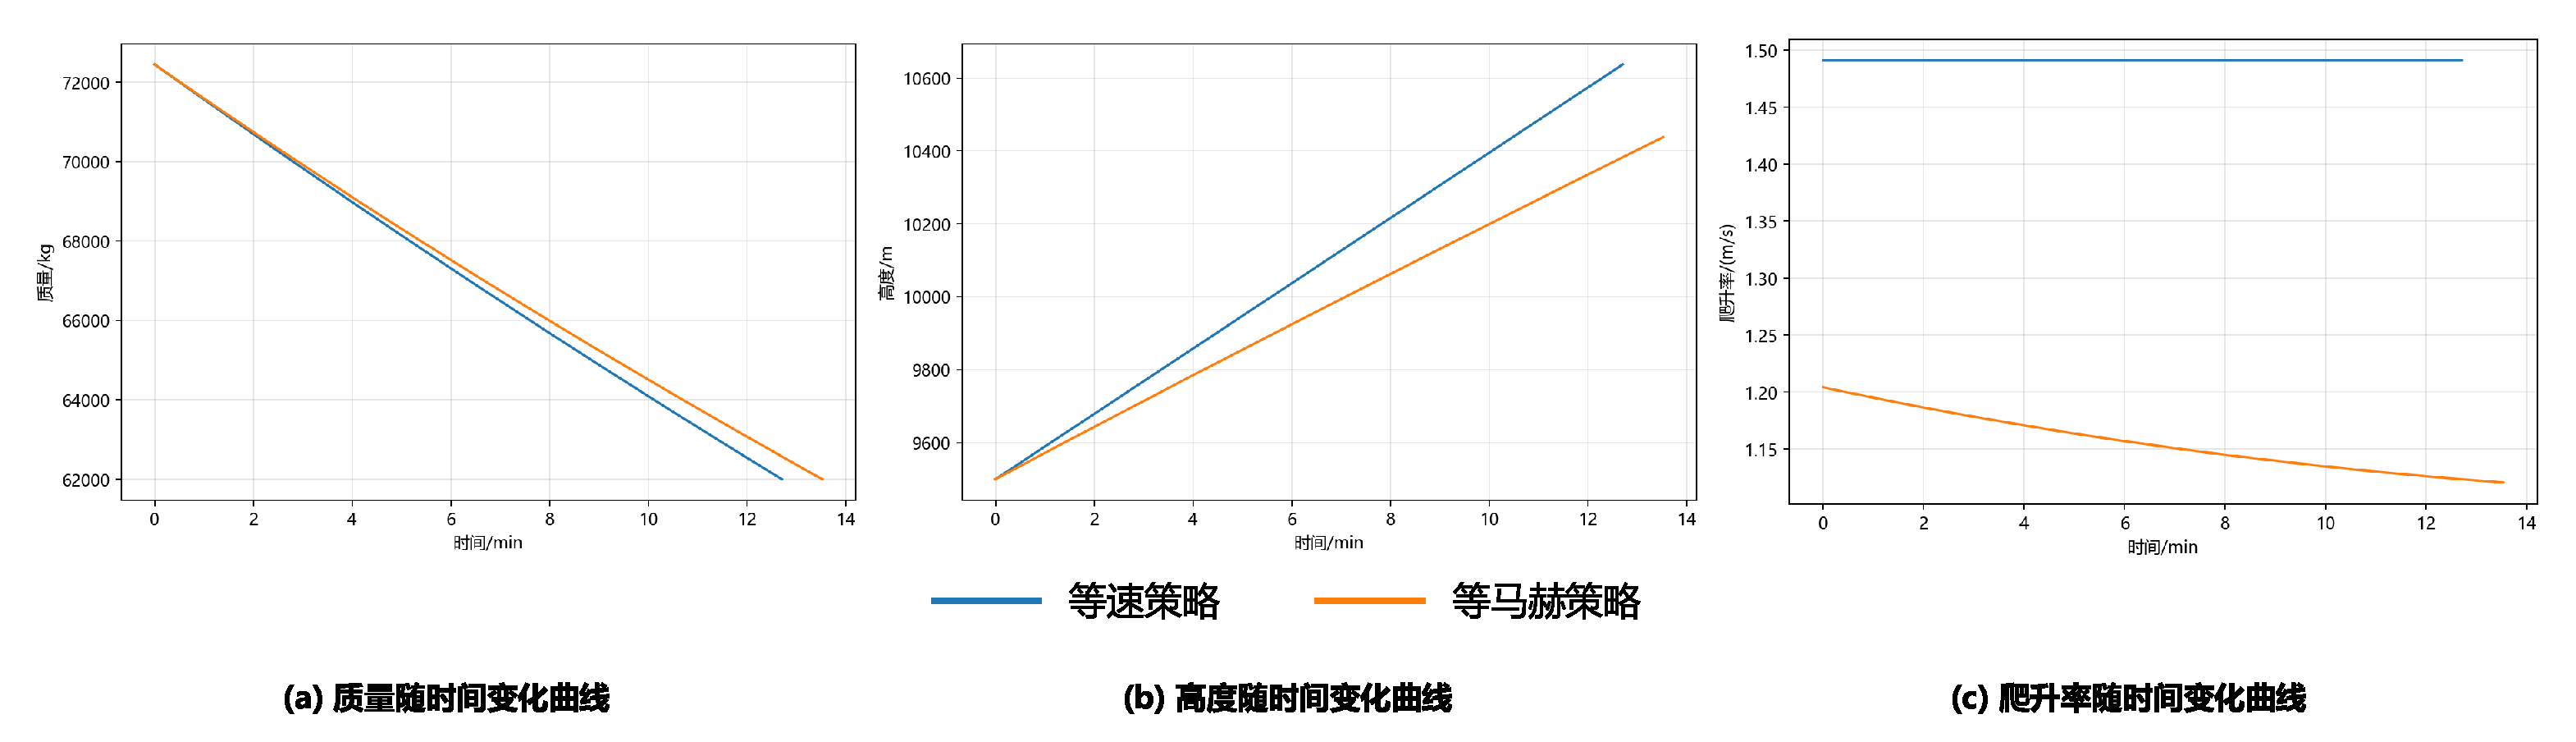
\includegraphics[width=1.1\textwidth]{2.eps}}{\fbox{Missing figure}}
	\caption{飞行状态参数随时间变化对比示意图}
	\label{fig:flight_state}
\end{figure}
由图(a)可知，两种策略的质量均从 $72450\text{ kg}$ 单调降至 $62000\text{ kg}$，因此总燃油消耗均为 $10450\text{ kg}$。由图(b)和图(c)可知，等速策略最终高度更高、平均爬升率更大，分别为 $10637.1\text{ m}$ 和 $1.49132\text{ m/s}$；等马赫数策略最终高度为 $10437.8\text{ m}$、平均爬升率为 $1.15553\text{ m/s}$。这说明在本文参数下，等速策略更有利于通过升高高度维持升力平衡，而等马赫数策略受温度变化影响更明显，爬升过程也更慢。

从飞行时间看，等速策略为 $12.7076\text{ min}$，等马赫数策略为 $13.5265\text{ min}$，差异主要来自等马赫数策略空速随声速降低而下降。综合来看，等速策略更快、更高，等马赫数策略则体现了速度约束与大气温度耦合后的响应特征。
\section{问题二模型建立与求解}
\subsection{模型建立}
\subsubsection{巡航全过程燃油消耗积分模型}

在问题一所建立的巡航动力学模型基础上，问题二进一步研究巡航全过程的燃油消耗量。
飞机在巡航过程中所处的大气环境随高度连续变化，因此燃油消耗率不再是常数，
而是高度、空速、质量以及大气参数共同作用下的非线性函数。

记单位时间燃油消耗率为
\begin{equation}
    \dot m_f(t)
    =
    c_fF(t)
    \left[
    1+\beta\left(V(t)-V_{\mathrm{opt}}\right)^2
    \right],
    \label{eq:q2_fuel_rate}
\end{equation}
其中推力需求 $F(t)$ 由问题一中的推力需求模型给出。于是，巡航全过程的总燃油消耗量可表示为：
\begin{equation}
    J
    =
    \int_{0}^{t_f}\dot m_f(t)\,\mathrm{d}t.
    \label{eq:q2_total_fuel_time}
\end{equation}

由于飞机水平运动方程为
\begin{equation}
    \dot x(t)=V(t)+W(h(t)),
    \label{eq:q2_xdot}
\end{equation}
当 $V(t)+W(h(t))>0$ 时，可将时间积分转化为沿飞行路径的积分形式：
\begin{equation}
    J
    =
    \int_{0}^{X_f}
    \frac{\dot m_f(x)}{V(x)+W(h(x))}\,\mathrm{d}x.
    \label{eq:q2_total_fuel_path}
\end{equation}
式 (60) 表明，巡航总油耗不仅与单位时间燃油消耗率有关，
还与飞机相对于地面的实际前进速度有关。若存在顺风，则相同空速下单位航程所需时间减少；
若存在逆风，则单位航程所需时间增加，从而影响总燃油消耗。
\subsubsection{燃油消耗率沿路径分布}

为绘制燃油消耗率沿飞行路径的分布曲线，可将时间域上的数值解
$h(t),V(t),m(t),x(t)$ 转换为路径坐标下的函数。定义单位航程燃油消耗率为
\begin{equation}
    q(x)
    =
    \frac{\dot m_f(x)}{V(x)+W(h(x))}.
    \label{eq:q2_fuel_per_distance}
\end{equation}
则总燃油消耗量可写为
\begin{equation}
    J=\int_{0}^{X_f}q(x)\,\mathrm{d}x.
    \label{eq:q2_total_q}
\end{equation}
其中，$q(x)$ 表示飞机每飞行单位地面距离所消耗的燃油质量。
相比于时间油耗率 $\dot m_f(t)$，该指标更能反映巡航策略在实际航程上的经济性。

\subsubsection{温度偏差修正模型}

实际大气温度可能与标准大气存在偏差。设实际温度为
\begin{equation}
    T_{\mathrm{real}}(h)
    =
    T_{\mathrm{std}}(h)+\Delta T(h),
    \label{eq:q2_T_real}
\end{equation}
其中，$\Delta T(h)$ 表示实际大气温度相对于标准大气温度的偏差。

当温度偏差较小时，本文采用一阶泰勒展开进行近似修正。由声速表达式可得
\begin{equation}
    a_{\Delta}(h)
    =
    \sqrt{\gamma R_{\mathrm{gas}}\left[T_{\mathrm{std}}(h)+\Delta T(h)\right]}
    =
    \sqrt{\gamma R_{\mathrm{gas}}\left[T_{\mathrm{std}}(h)\right]}\sqrt{1+\frac{\Delta T(h)}{T_{\mathrm{std}}(h)}}
    \approx
    a(h)
    \left[
    1+\frac{\Delta T(h)}{2T_{\mathrm{std}}(h)}
    \right].
    \label{eq:q2_a_delta}
\end{equation}

在局部压力近似不变的条件下，由理想气体状态方程可得大气密度的一阶修正形式：
\begin{equation}
    \rho_{\Delta}(h)
    \approx
    \rho(h)
    \left[
    1-\frac{\Delta T(h)}{T_{\mathrm{std}}(h)}
    \right].
    \label{eq:q2_rho_delta}
\end{equation}
该近似表明，在同一高度附近，温度升高会导致密度降低，从而改变升力、阻力以及推力需求。

将修正后的密度 $\rho_{\Delta}(h)$ 代入升力和阻力模型，可得到修正后的阻力
$D_{\Delta}(t)$ 和推力需求 $F_{\Delta}(t)$。因此，温度偏差修正后的燃油消耗率为
\begin{equation}
    \dot m_{f,\Delta}(t)
    =
    c_fF_{\Delta}(t)
    \left[
    1+\beta\left(V(t)-V_{\mathrm{opt}}\right)^2
    \right].
    \label{eq:q2_fuel_delta}
\end{equation}
若采用等马赫数策略，则空速还需由修正后的声速确定，即
\begin{equation}
    V_{\Delta}(t)=M_0a_{\Delta}(h(t)).
    \label{eq:q2_V_delta}
\end{equation}

最终，修正后的总燃油消耗量为
\begin{equation}
    J_{\Delta}
    =
    \int_{0}^{t_f}\dot m_{f,\Delta}(t)\,\mathrm{d}t
    =
    \int_{0}^{X_f}
    \frac{\dot m_{f,\Delta}(x)}{V(x)+W(h(x))}\,\mathrm{d}x.
    \label{eq:q2_total_delta}
\end{equation}
通过比较 $J_{\Delta}$ 与标准大气条件下的 $J$，即可分析温度偏差对巡航油耗计算结果的影响。
当 $\left|\Delta T(h)\right|/T_{\mathrm{std}}(h)$ 较小，且其引起的油耗变化远小于工程允许误差时，
可安全忽略温度偏差；反之，则应采用修正后的大气参数重新计算油耗。
\subsection{模型求解}
基于路径积分模型，本文选取问题一中的等速巡航爬升轨迹作为标准大气下的基准轨迹。该轨迹包含$h(t)$、$V(t)$、$m(t)$、$\dot m_f(t)$ 和 $x(t)$等变量。将时间域结果转换为路径坐标后，逐点计算单位航程燃油消耗率 $q(x)$，并采用梯形积分法计算巡航全过程总油耗。
具体求解步骤如下。

首先，读取问题一得到的等速巡航剖面。对每一个离散节点 $i$，已知飞机高度 $h_i$、空速 $V_i$、质量 $m_i$、燃油消耗率 $\dot m_{f,i}$ 和累计航程 $x_i$。由水平运动方程计算地速：
$$U_i=V_i+W(h_i).$$

随后，根据式（61）中的单位航程油耗率定义，计算
$$q_i=\frac{\dot m_{f,i}}{U_i}.$$

最后，采用梯形积分得到标准大气条件下的累计燃油消耗量：
$$J(x_j)\approx \sum_{i=0}^{j-1}\frac{q_i+q_{i+1}}{2}(x_{i+1}-x_i).$$
当 $x_j=X_f$ 时，即得到该巡航策略在标准大气条件下的全过程总油耗 $J$。

在大气参数处理上，等速策略主要体现密度 $\rho(h)$ 和风场 $W(h)$对路径油耗的影响；等马赫数策略中速度满足 $V=M a(h)$，因此进一步体现了声速随高度变化对飞行状态和路径油耗计算的影响。两种轨迹共同用于验证大气参数高度分布对油耗积分结果的影响。
\begin{figure}[H]
	\centering
	\IfFileExists{3.eps}{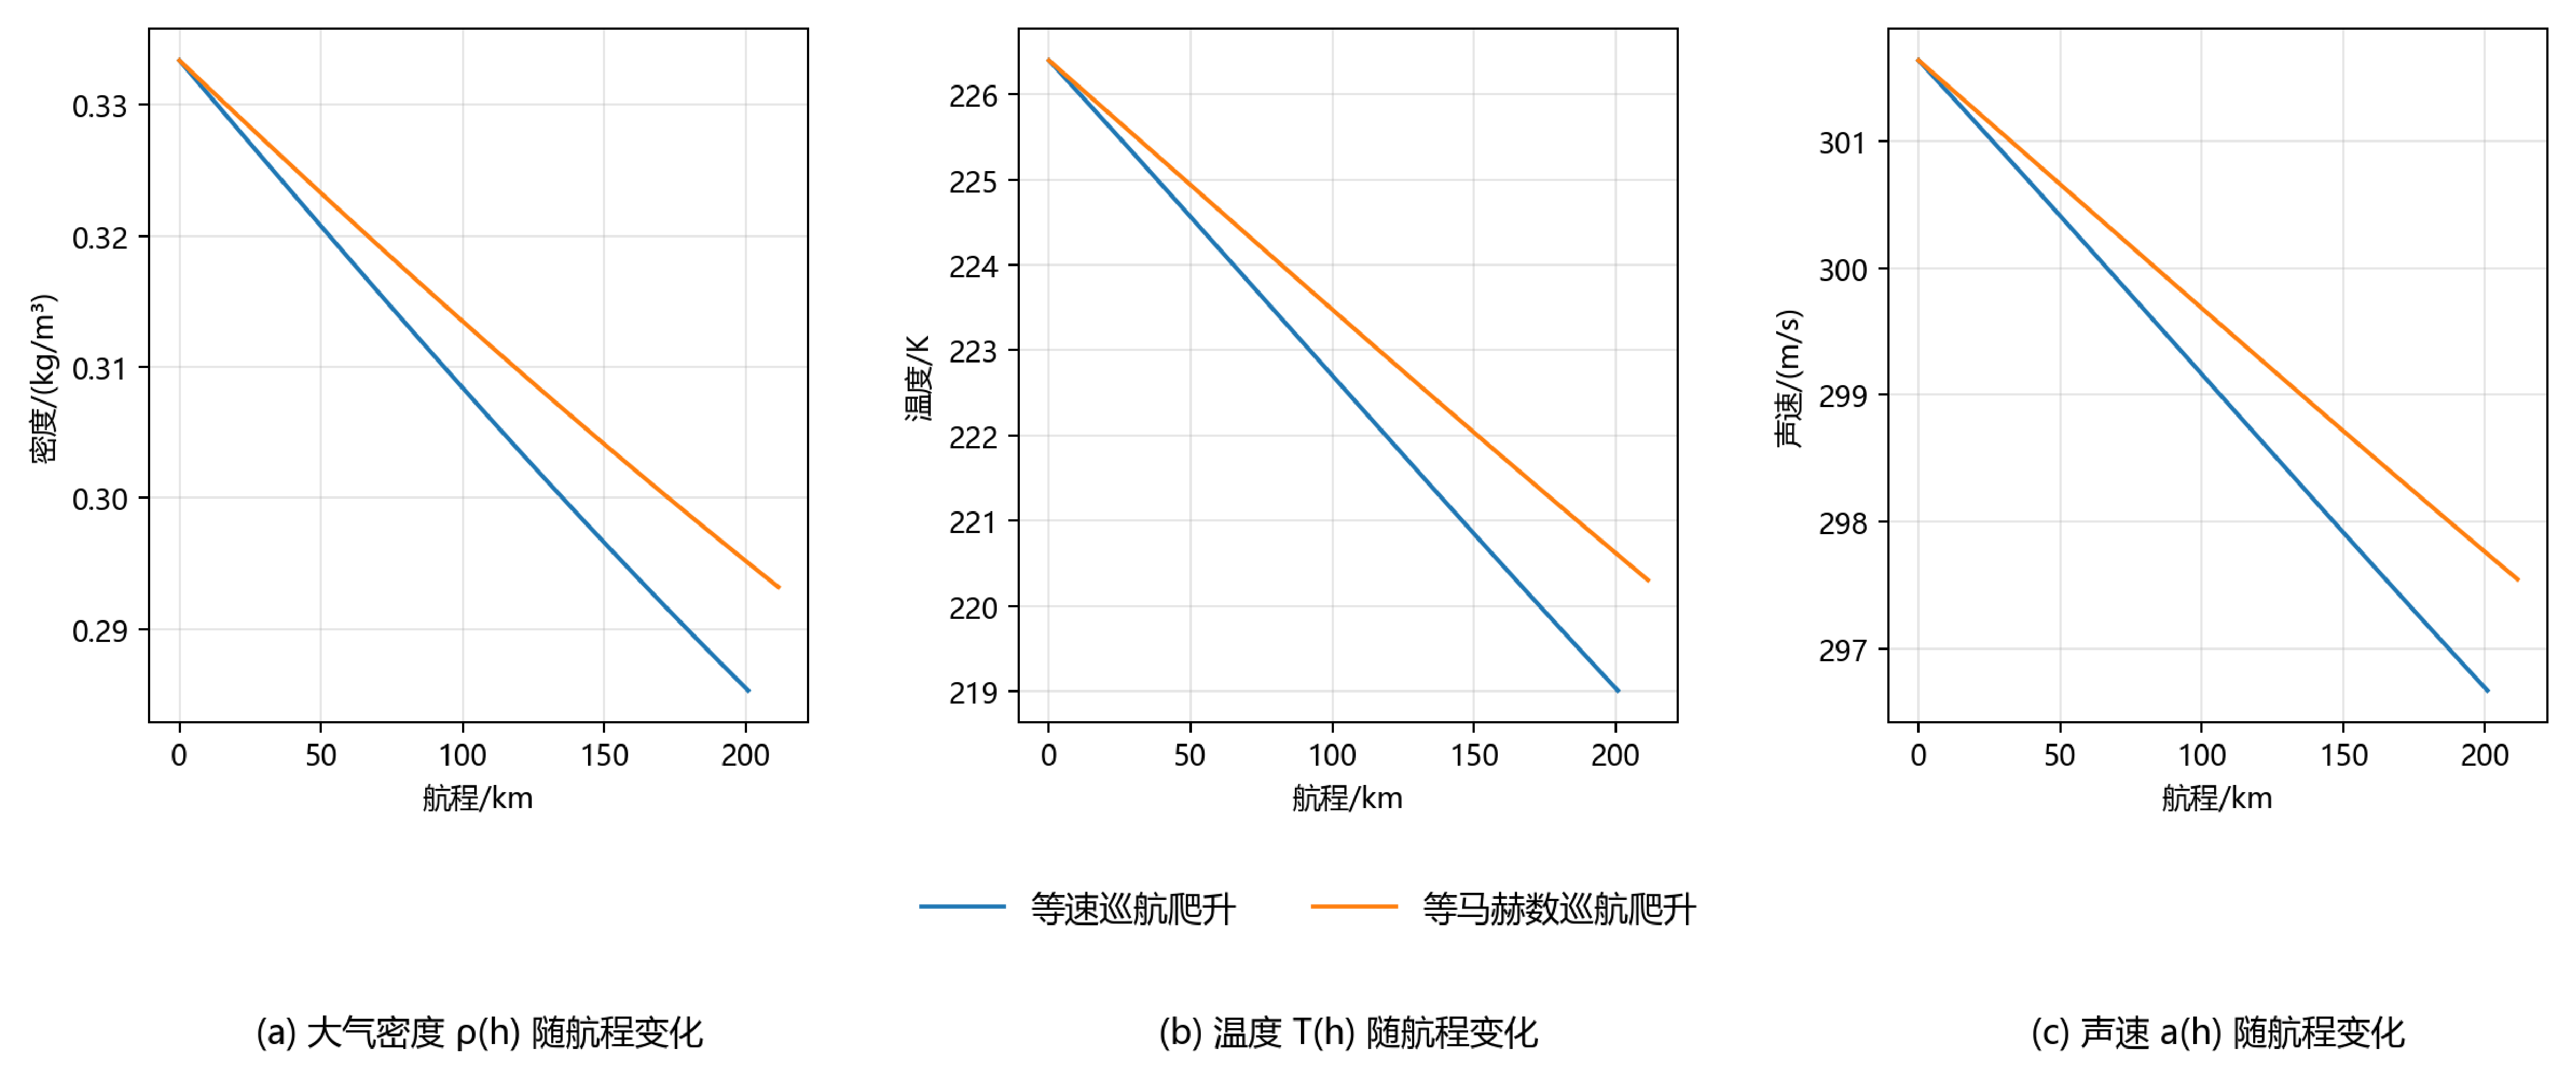
\includegraphics[width=1\textwidth]{3.eps}}{\fbox{Missing figure}}
	\caption{温度、密度和声速与航程关系图}
	\label{fig:atmosphere}
\end{figure}

由图3可知，随着巡航爬升过程推进，大气密度、温度和声速均沿航程连续下降。等速策略最终高度更高，因此对应的大气密度、温度和声速下降幅度更大；等马赫数策略高度增长较缓，三类大气参数变化幅度相对较小。该结果说明飞机并非在单一大气状态下飞行，而是在随高度连续变化的参数场中完成路径积分。

针对实际大气温度偏差，本文采用一阶扰动近似进行修正。并分别设置恒定温度偏差 $\Delta T=5K$，和线性温差 $\Delta T(h)=5+0.0005(h-h_0)$。在每个路径节点上，利用式（64）和式（65）更新声速和密度，再重新计算阻力、推力、燃油消耗率和单位航程油耗率，最终得到修正后的总燃油消耗量 $J_\Delta$。
\subsection{结果分析}
两种巡航策略在标准大气及温度偏差修正条件下的总油耗结果如下表所示。
\begin{table}[htbp]
\centering
\caption{不同巡航策略与大气条件下的油耗对比}
\label{tab:fuel_comparison}
\begin{tabular}{ccccccc}
\toprule
策略 & 情形 & 总油耗/kg & 油耗变化/kg &  平均单位航程油耗/(kg/m) \\
\midrule
等速爬升 & 标准大气 & 10450 & 0 &  0.052039 \\
等速爬升 & 恒定5K温差 & 10439.5 & -10.4968 &  0.051987 \\
等速爬升 & 线性温差 & 10439.1 & -10.9384 &  0.051985 \\
等马赫数爬升 & 标准大气 & 10450 & 0 &  0.049414 \\
等马赫数爬升 & 恒定5K温差 & 10439.3 & -10.7486 &  0.049363 \\
等马赫数爬升 & 线性温差 & 10438.9 & -11.1239 &  0.049362 \\
\bottomrule
\end{tabular}
\end{table}

由表可知，标准大气条件下两种策略的总油耗均为 $10450.0\text{ kg}$，与由初始质量和终止质量计算得到的结果一致，说明路径积分模型与质量变化模型相互吻合。图4表明，等马赫数策略的平均单位航程油耗更低，为 $0.049414\text{ kg/m}$，而等速策略为 $0.052039\text{ kg/m}$，差异主要来自等马赫数策略航程更长、单位航程分摊后的平均油耗更小。

\begin{figure}[H]
	\centering
	\IfFileExists{4.eps}{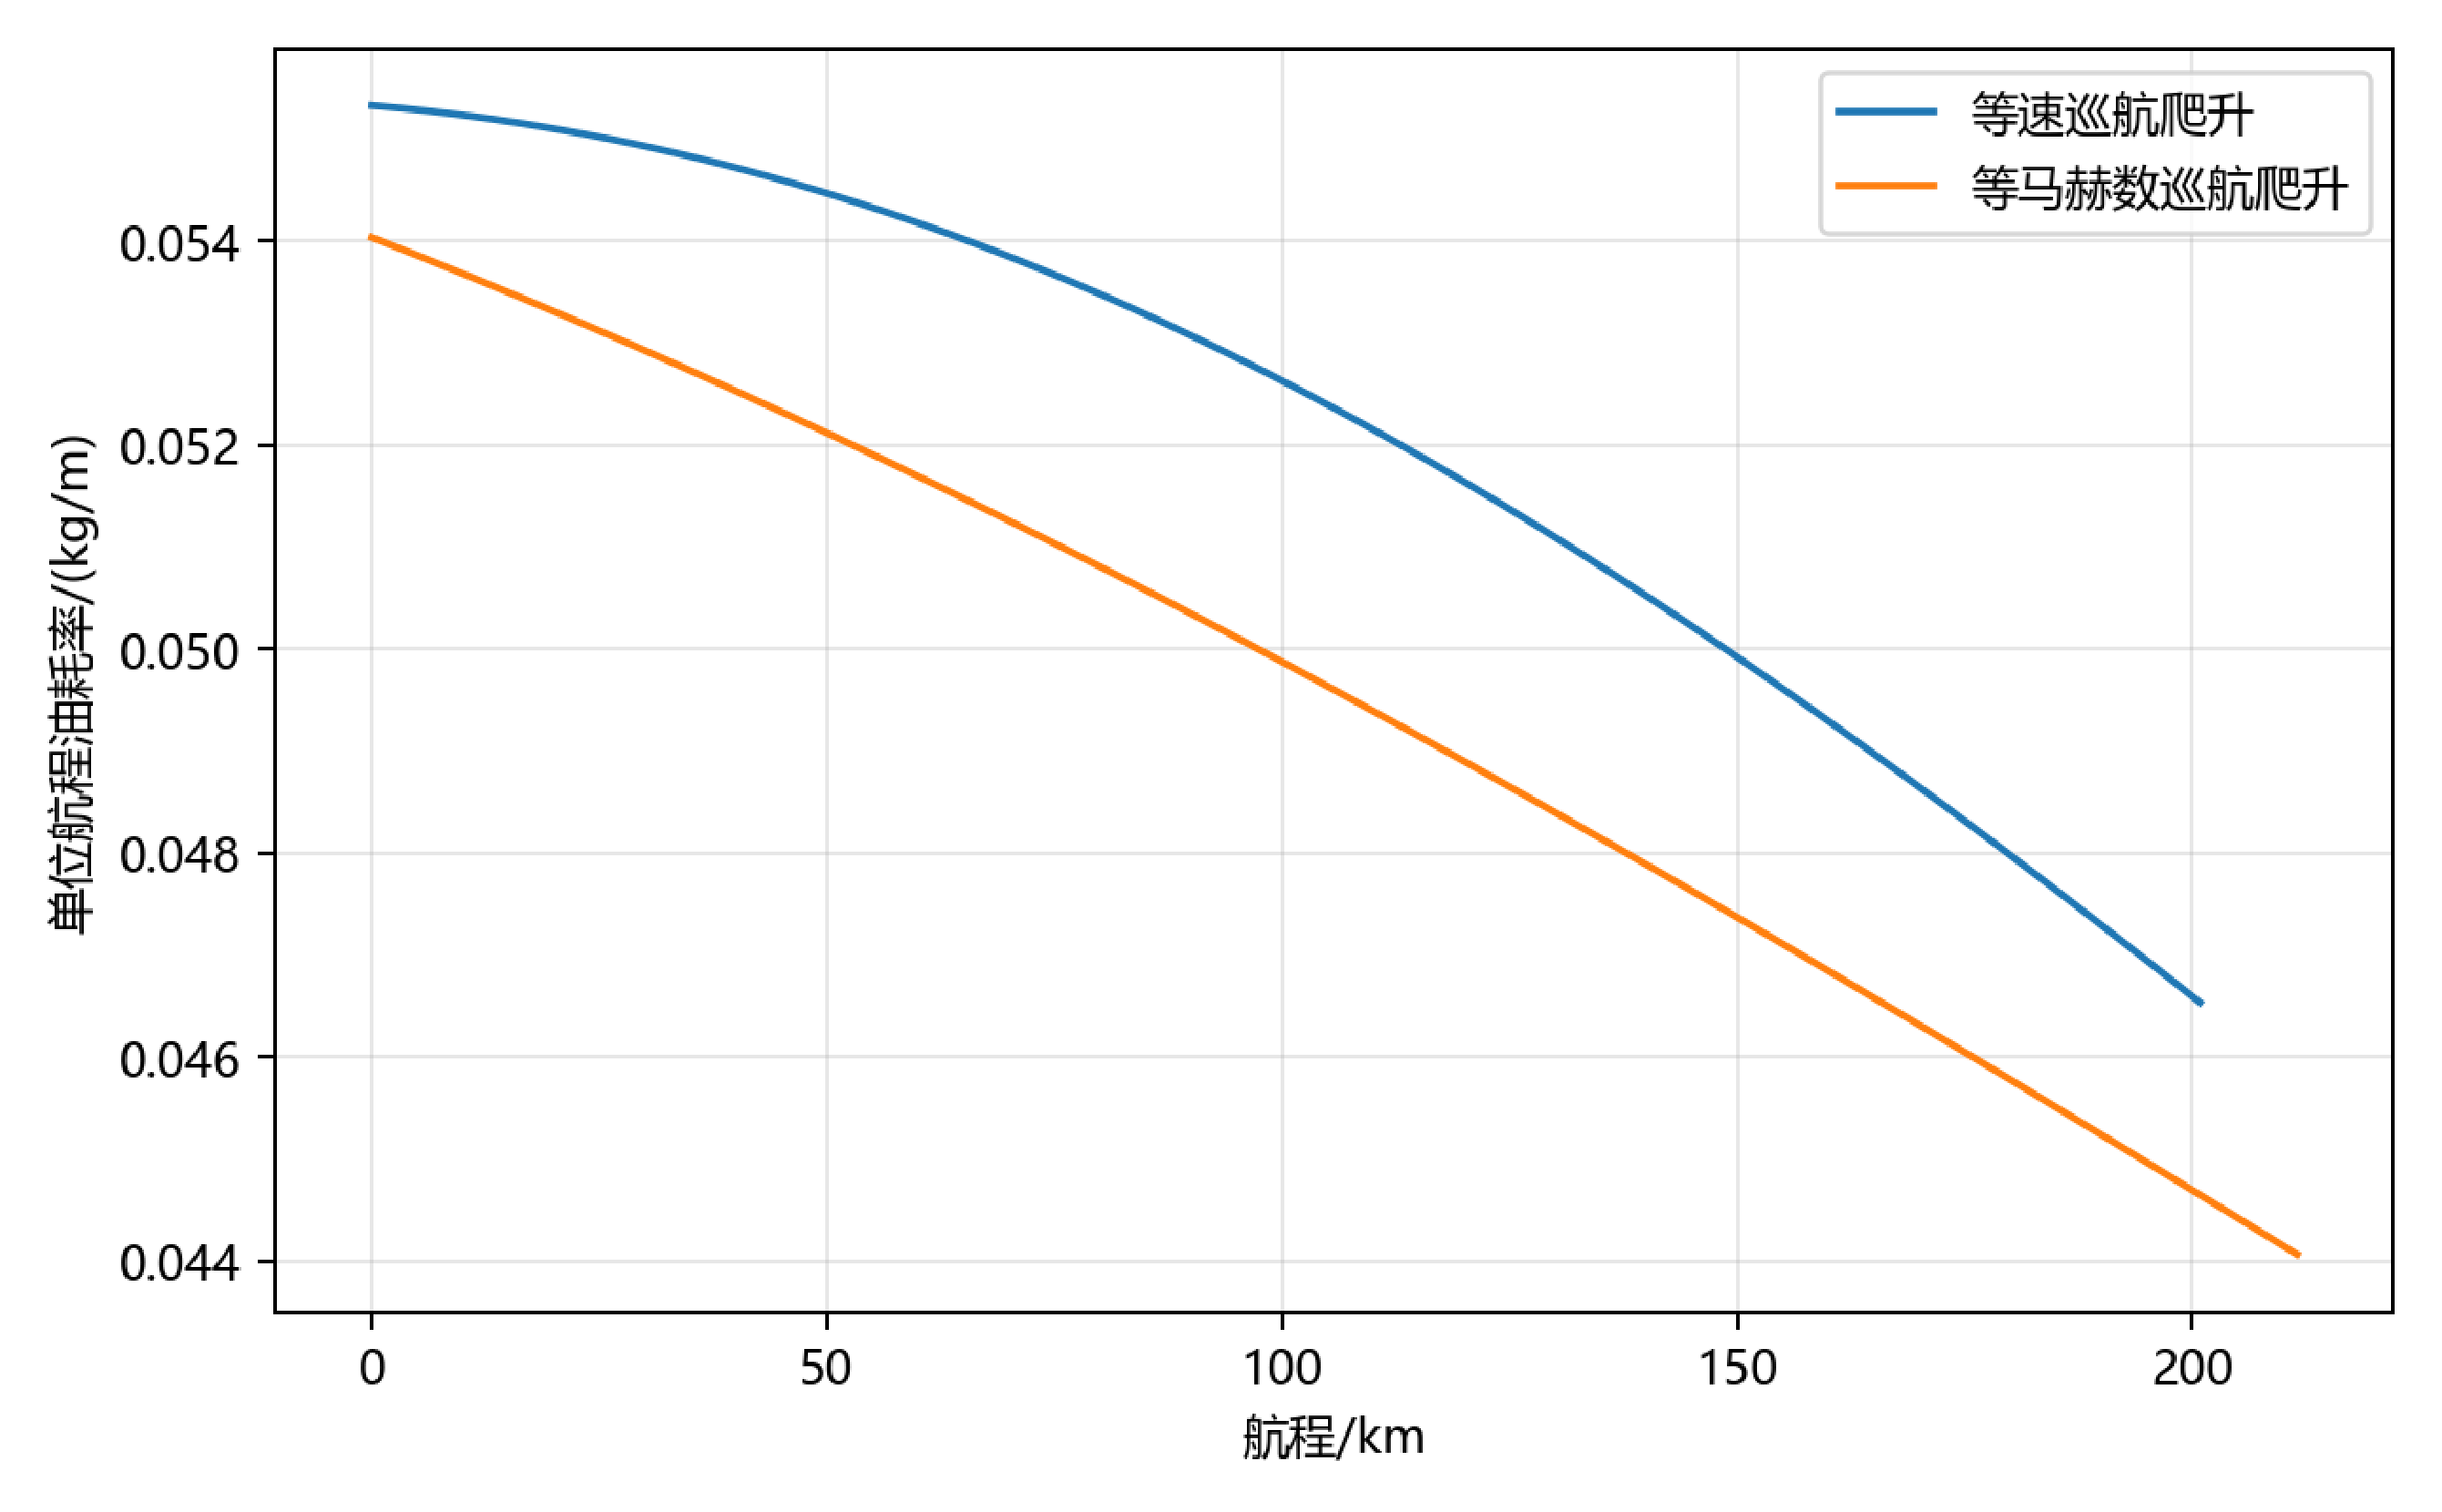
\includegraphics[width=0.7\textwidth]{4.eps}}{\fbox{Missing figure}}
	\caption{标准大气条件下单位航程油耗率沿路径分布}
	\label{fig:nx}
\end{figure}
进一步看，单位航程油耗率并非常数，而是随质量、高度、阻力和地速变化连续调整，说明路径油耗本质上是大气参数与飞行状态共同作用的结果。

\begin{figure}[H]
	\centering
	\IfFileExists{5.eps}{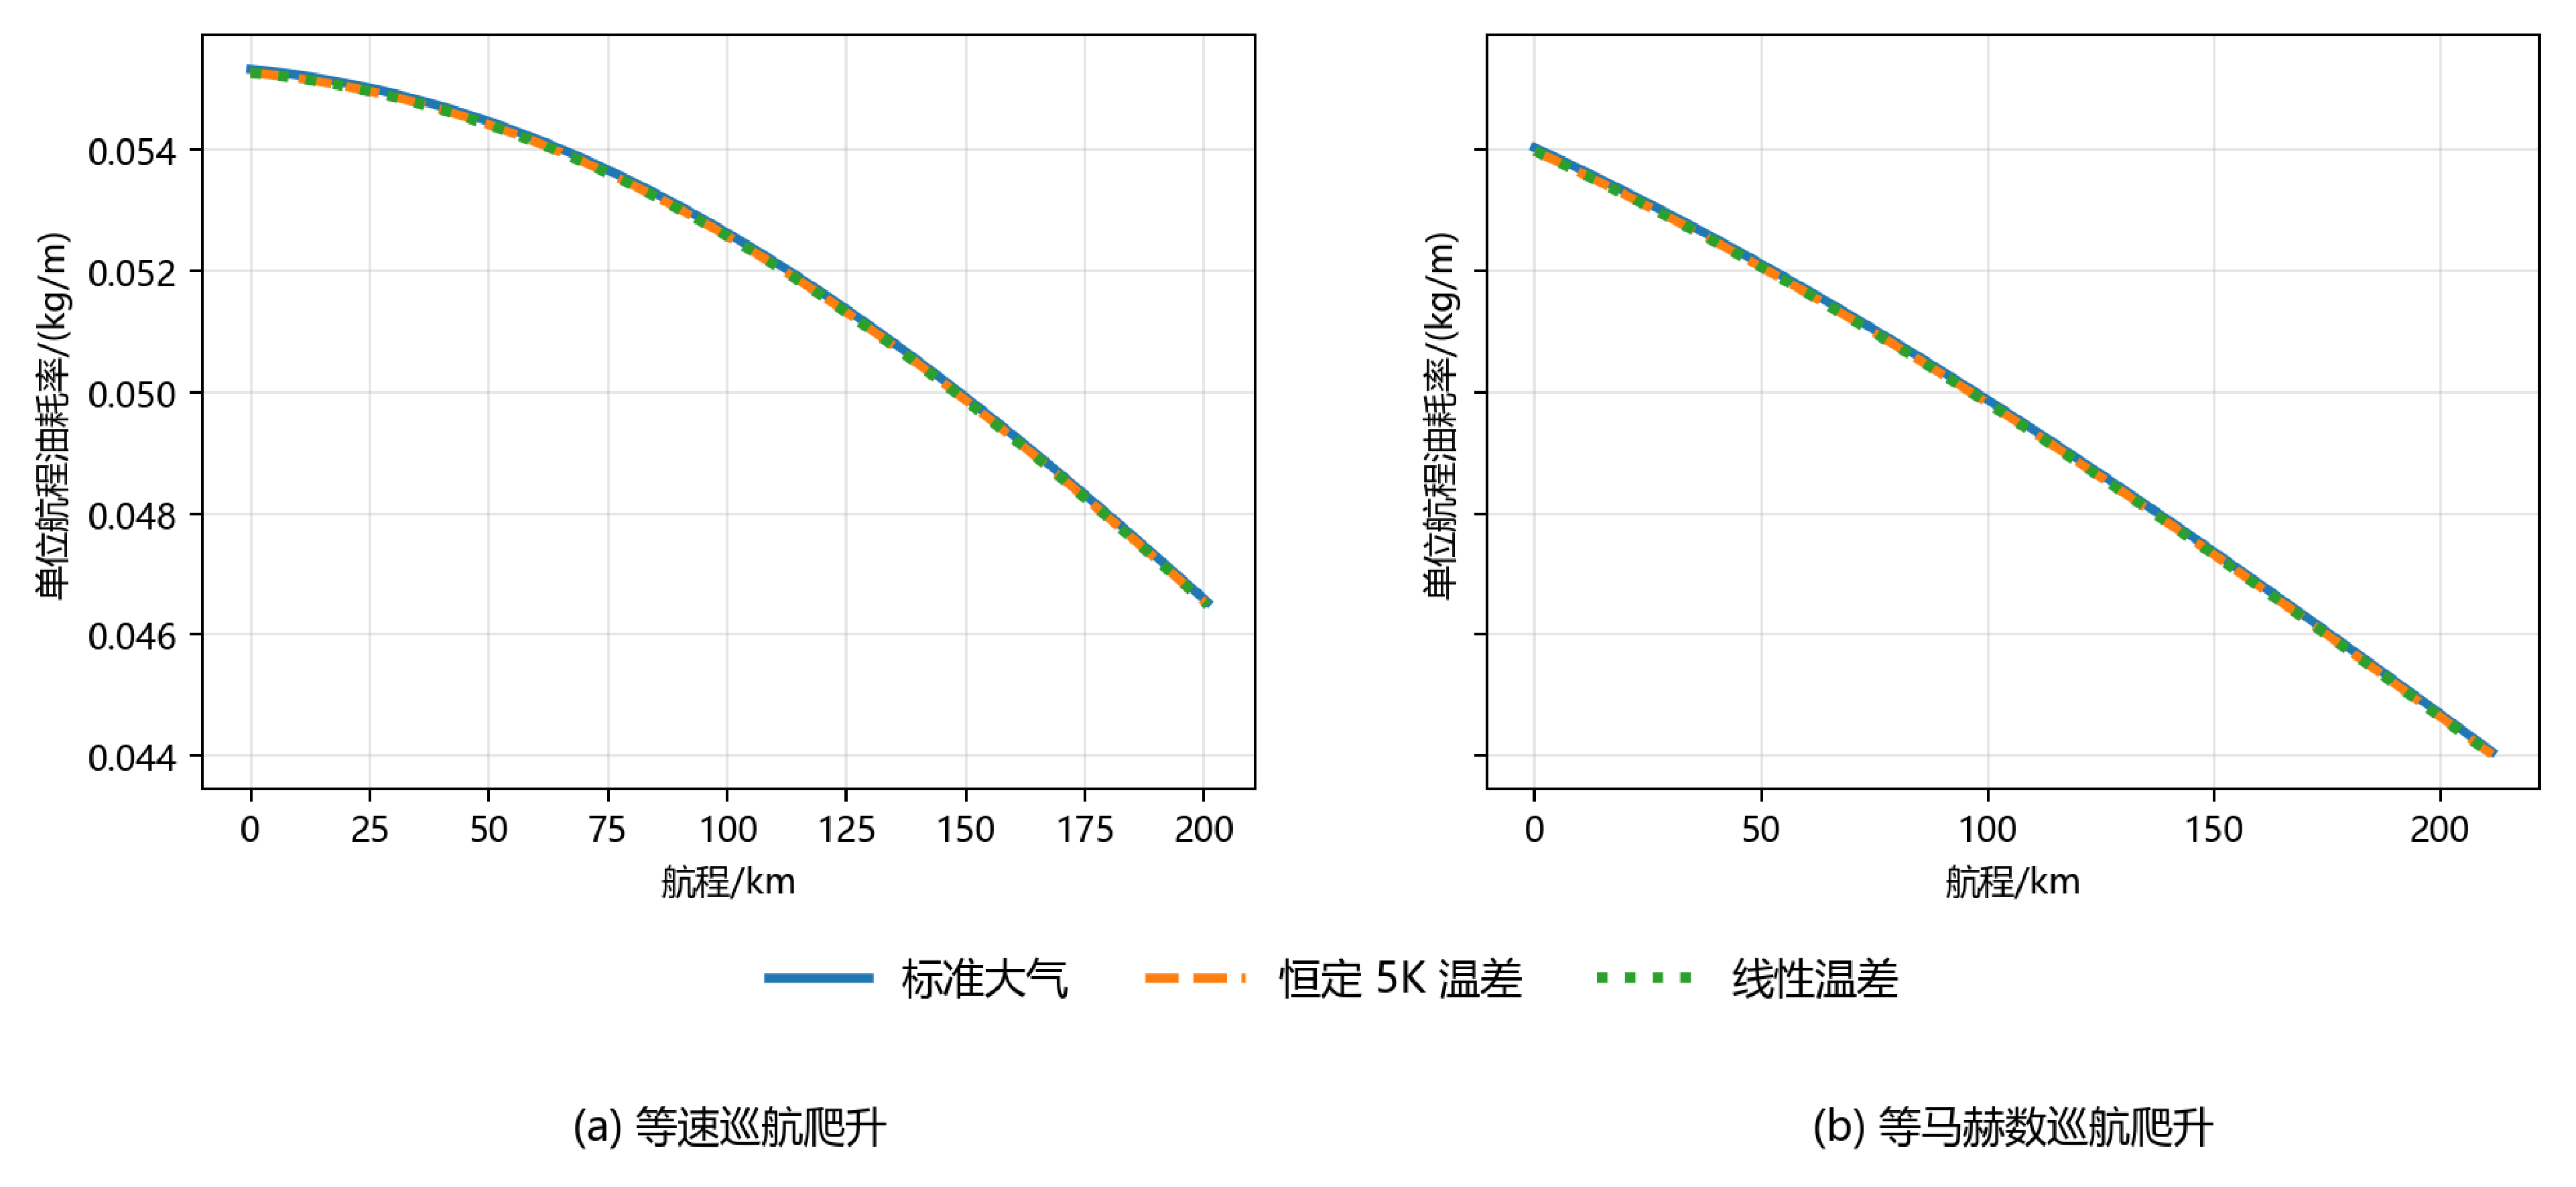
\includegraphics[width=1\textwidth]{5.eps}}{\fbox{Missing figure}}
	\caption{温度偏差修正前后单位航程油耗率对比}
	\label{fig:nx1}
\end{figure}
图5显示，恒定 $5K$ 温差和线性温差下两种策略的总油耗变化都只有约 $0.1\%$，说明在本题给定高度范围内，温度偏差对总油耗影响较弱。其原因是温度扰动主要通过密度和声速进入模型，但扰动幅度较小，传递到阻力、推力和油耗后被进一步削弱。

因此，问题二的结论可以概括为：路径积分模型与质量变化模型一致，单位航程油耗更能反映巡航经济性，而温度偏差在当前工况下只带来小幅修正，对策略优劣判断影响有限。
\section{问题三模型建立与求解}
\subsection{模型建立}
\subsubsection{最优巡航控制模型}

问题三要求在给定初始飞行状态下，确定使巡航总燃油消耗最小的高度--速度联合变化规律。
由于飞机高度、速度、质量和阻力之间存在非线性耦合关系，本文将其建模为连续时间最优控制问题。

为避免推力模型中同时出现 $h(t)$、$V(t)$ 及其导数造成表达不便，本文将飞行高度和空速也纳入状态变量，
并引入高度变化率和空速变化率作为控制变量：
\begin{equation}
    u_h(t)=\dot h(t),\qquad u_V(t)=\dot V(t).
    \label{eq:q3_controls}
\end{equation}
于是，状态变量选为
\begin{equation}
    \boldsymbol{y}(t)=\left[x(t),m(t),h(t),V(t)\right]^{\mathrm T},
    \label{eq:q3_states}
\end{equation}
控制变量选为
\begin{equation}
    \boldsymbol{u}(t)=\left[u_h(t),u_V(t)\right]^{\mathrm T}.
    \label{eq:q3_control_vector}
\end{equation}

在此表示下，推力需求模型可写为
\begin{equation}
    F(t)
    =
    D(t)+m(t)u_V(t)+\frac{m(t)g}{V(t)}u_h(t).
    \label{eq:q3_thrust}
\end{equation}
燃油消耗率为
\begin{equation}
    \phi(t)
    =
    c_fF(t)
    \left[
    1+\beta\left(V(t)-V_{\mathrm{opt}}\right)^2
    \right].
    \label{eq:q3_phi}
\end{equation}
其中，$\phi(t)$ 即为单位时间燃油消耗率。

因此，巡航过程的状态方程组可写为
\begin{equation}
\left\{
\begin{aligned}
    \dot x(t) &= V(t)+W(h(t)),\\
    \dot m(t) &= -\phi(t),\\
    \dot h(t) &= u_h(t),\\
    \dot V(t) &= u_V(t).
\end{aligned}
\right.
\label{eq:q3_state_equations}
\end{equation}

若给定巡航航程 $X_f$，则总燃油消耗最小问题可表示为
\begin{equation}
    \min_{\boldsymbol{u}(t),\,t_f}
    J
    =
    \int_{0}^{t_f}\phi(t)\,\mathrm{d}t.
    \label{eq:q3_objective}
\end{equation}

对应的初始条件和终止条件为
\begin{equation}
    x(0)=0,\quad m(0)=m_0,\quad h(0)=h_0,\quad V(0)=V_0,
    \label{eq:q3_initial}
\end{equation}
\begin{equation}
    x(t_f)=X_f,\qquad m(t_f)\geq m_f.
    \label{eq:q3_terminal}
\end{equation}
其中，$X_f$ 表示给定巡航航程，$m_f$ 表示终止时允许的最小剩余质量。

\subsubsection{约束条件}

飞机巡航轨迹应满足飞行包线、升力平衡、马赫数以及推力非负等约束。
首先，高度和速度需满足
\begin{equation}
    h_{\min}\leq h(t)\leq h_{\max},
    \qquad
    V_{\min}\leq V(t)\leq V_{\max}.
    \label{eq:q3_hV_bounds}
\end{equation}

马赫数需满足跨音速限制：
\begin{equation}
    M(t)=\frac{V(t)}{a(h(t))}\leq M_{\max}.
    \label{eq:q3_mach_constraint}
\end{equation}

升力系数由升力平衡确定，为
\begin{equation}
    C_L(t)=\frac{2m(t)g}{\rho(h(t))V^2(t)S}.
    \label{eq:q3_CL}
\end{equation}
为保证飞机处于合理升力工作范围，设置
\begin{equation}
    C_{L,\min}\leq C_L(t)\leq C_{L,\max}.
    \label{eq:q3_CL_bounds}
\end{equation}

考虑到乘坐品质和结构安全，还需对爬升率和水平加速度进行限制：
\begin{equation}
    |\dot h(t)| \leq \dot h_{\max}, \qquad |\dot V(t)| \leq \dot V_{\max},
\end{equation}
其中 $\dot h_{\max}=15\,\text{m/s}$，$\dot V_{\max}=1.0\,\text{m/s}^2$

此外，发动机推力应满足
\begin{equation}
    0\leq F(t)\leq F_{\max}(h(t),V(t)).
    \label{eq:q3_thrust_constraint}
\end{equation}
若题目未给出最大推力包线，则可在基础模型中仅保留 $F(t)\geq0$，并在模型改进中进一步引入发动机推力上限。

\subsubsection{最优性必要条件}

为分析最优轨迹满足的数学条件，引入伴随变量
\[
\lambda_x(t),\lambda_m(t),\lambda_h(t),\lambda_V(t),
\]
构造哈密顿函数
\begin{equation}
\begin{aligned}
    \mathcal H
    &=
    \phi(t)
    +\lambda_x(t)\left[V(t)+W(h(t))\right]
    -\lambda_m(t)\phi(t) \\
    &\quad
    +\lambda_h(t)u_h(t)
    +\lambda_V(t)u_V(t).
\end{aligned}
\label{eq:q3_Hamiltonian}
\end{equation}
整理可得
\begin{equation}
    \mathcal H
    =
    \left[1-\lambda_m(t)\right]\phi(t)
    +\lambda_x(t)\left[V(t)+W(h(t))\right]
    +\lambda_h(t)u_h(t)
    +\lambda_V(t)u_V(t).
    \label{eq:q3_Hamiltonian_simple}
\end{equation}

对于内部最优解，其伴随方程满足
\begin{equation}
    \dot{\lambda}_i(t)
    =
    -\frac{\partial \mathcal H}{\partial y_i},
    \qquad
    y_i\in\{x,m,h,V\}.
    \label{eq:q3_adjoint}
\end{equation}
即
\begin{equation}
\left\{
\begin{aligned}
    \dot\lambda_x(t)&=-\frac{\partial \mathcal H}{\partial x},\\
    \dot\lambda_m(t)&=-\frac{\partial \mathcal H}{\partial m},\\
    \dot\lambda_h(t)&=-\frac{\partial \mathcal H}{\partial h},\\
    \dot\lambda_V(t)&=-\frac{\partial \mathcal H}{\partial V}.
\end{aligned}
\right.
\label{eq:q3_adjoint_system}
\end{equation}

同时，控制变量需满足驻值条件
\begin{equation}
    \frac{\partial \mathcal H}{\partial u_h}=0,
    \qquad
    \frac{\partial \mathcal H}{\partial u_V}=0.
    \label{eq:q3_stationary}
\end{equation}
当高度、速度、升力系数或推力约束处于边界时，上述驻值条件需替换为包含不等式约束乘子的
KKT 条件。
\subsection{参数取值与依据}
\label{sec:params}

本文参考同类机型性能数据\cite{11}\cite{12}、飞行包线理论\cite{10}及乘坐品质标准\cite{12}，设定各约束参数如表4所示。

\begin{table}[htbp]
\centering
\caption{约束参数取值}
\label{tab:const_params}
\begin{tabular}{cccc}
\toprule
参数 & 符号 & 取值 & 依据 \\
\midrule
最低高度 & $h_{\min}$ & 8000 m & 安全高度与航线最低航路高度 \\
最高高度 & $h_{\max}$ & 12000 m & 飞机升限及发动机推力限制 \\
最小空速 & $V_{\min}$ & 180 m/s & 失速速度 \\
最大空速 & $V_{\max}$ & 280 m/s & 结构限制与跨音速边界 \\
最大马赫数 & $M_{\max}$ & 0.85 & 阻力发散马赫数 \\
最小升力系数 & $C_{L,\min}$ & 0.1 & 迎角过低时操纵性问题 \\
最大升力系数 & $C_{L,\max}$ & 1.2 & 失速迎角对应升力系数 \\
最大爬升率 & $\dot h_{\max}$ & 15 m/s & 乘坐品质与结构载荷 \\
最大水平加速度 & $\dot V_{\max}$ & 1.0 m/s$^2$ & 乘坐舒适度与发动机响应 \\
\bottomrule
\end{tabular}
\end{table}
\subsection{模型求解}
\subsubsection{直接离散化求解模型}
由于本问题的燃油消耗率、阻力模型和风场模型均具有明显非线性，采用间接法求解两点边值问题较为困难。
因此，本文采用直接法进行数值求解。将时间区间 $[0,t_f]$ 划分为 $N$ 个小区间，
节点记为 $t_i=i\Delta t$，$i=0,1,\ldots,N$。

采用梯形积分近似，可将目标函数离散为
\begin{equation}
    J
    \approx
    \sum_{i=0}^{N-1}
    \frac{\Delta t}{2}
    \left[
    \phi_i+\phi_{i+1}
    \right].
    \label{eq:q3_discrete_objective}
\end{equation}
  
状态方程离散为
\begin{equation}
    \boldsymbol y_{i+1}
    =
    \boldsymbol y_i
    +
    \frac{\Delta t}{2}
    \left[
    \boldsymbol f(\boldsymbol y_i,\boldsymbol u_i)
    +
    \boldsymbol f(\boldsymbol y_{i+1},\boldsymbol u_{i+1})
    \right],
    \label{eq:q3_trapezoid}
\end{equation}
其中，$\boldsymbol f$ 表示式 (76) 右端函数。
这样即可将连续最优控制问题转化为带非线性等式与不等式约束的非线性规划问题。

根据时间域梯形配点法的求解结果，本文分别得到无风条件和垂直风切变条件下的高度--速度联合最优巡航轨迹。两种工况均采用相同固定航程 $X_f=182988.940\text{ m}$。该航程取自无风等速巡航爬升基准策略由初始质量 $m_0$飞行至终止剩余质量 $m_f$时对应的航程。在该设置下，无风条件和垂直风切变条件均完成相同航程任务，使两种工况下的高度轨迹、速度轨迹、飞行时间和总燃油消耗具有可比性。

同时，若直接令 $m(t_f)=m_f$，则总燃油消耗$m_0-m_f$ 被预先固定，最小油耗目标将失去优化意义。因此，本文采用固定航程最小油耗形式，并将终端质量设置为安全剩余质量约束。离散后的问题属于带非线性等式约束和不等式约束的非线性规划问题，本文采用 SLSQP 算法进行求解。SLSQP 即序列最小二乘二次规划方法，能够同时处理变量边界、等式约束和不等式约束，适合本文包含配点动力学约束、飞行包线约束、终端巡航状态约束和最小推力约束的最优控制问题。

\subsubsection{风场对最优解结构的影响}

在无风条件下，$W(h)=0$，飞机地速等于空速，水平运动方程不再显式依赖高度。
此时可引入能量高度\cite{4}
\begin{equation}
    E_{\mathrm{tot}}(t)
    =
    h(t)+\frac{V^2(t)}{2g}.
    \label{eq:q3_energy_height}
\end{equation}
其变化率为
\begin{equation}
    \dot E_{\mathrm{tot}}(t)
    =
    \dot h(t)+\frac{V(t)}{g}\dot V(t).
    \label{eq:q3_Edot}
\end{equation}
结合推力需求模型可知，无风条件下高度变化和速度变化可通过能量高度统一描述，
从而在一定条件下将高度--速度二维控制问题简化为能量高度的一维决策问题。

然而，当存在垂直风切变时，风速 $W(h)$ 显式出现在水平运动方程中，
并通过路径积分中的 $V(t)+W(h(t))$ 影响单位航程燃油消耗。
此时，即使能量高度相同，不同高度对应的风速也可能不同，导致相同能量状态下的地速和单位航程油耗不同。
因此，风场破坏了无风条件下高度与速度之间的简化关系，使最优轨迹必须同时考虑气动效率、
速度偏离损失和风场收益。
\subsection{结果分析}
\begin{table}[htbp]
\centering
\caption{三种巡航策略下飞机空速随航程变化曲线}
\label{tab:opt_results_wind}
\begin{tabular}{ccccccc}
\toprule
工况 & 总油耗/kg & 终端质量/kg & 总飞行时间/s & 最大约束残差 \\
\midrule
无风最优轨迹 & 8947.394 & 63502.606 & 777.724& $2.900\times10^{-8}$ \\
有风最优轨迹 & 7707.451 & 64742.549 & 660.884& $4.013\times10^{-8}$ \\
\bottomrule
\end{tabular}
\end{table}

由表 5 可知，两种工况下优化器均正常收敛，最大约束残差接近 0，说明数值轨迹满足动力学方程及各类路径约束。无风条件下最优总油耗为 $8947.394\text{ kg}$，有风条件下为 $7707.451\text{ kg}$，节油率约 $13.86\%$；对应飞行时间由 $777.724\text{ s}$ 缩短至 $660.884\text{ s}$，降幅约 $15.02\%$。

这表明风场的主要作用不是显著降低单位时间燃油率，而是通过提高地速缩短固定航程所需时间。也就是说，有风最优轨迹的优势主要来自路径时间压缩，而不是发动机瞬时油耗的大幅下降。

\begin{figure}[H]
	\centering
	\IfFileExists{6.eps}{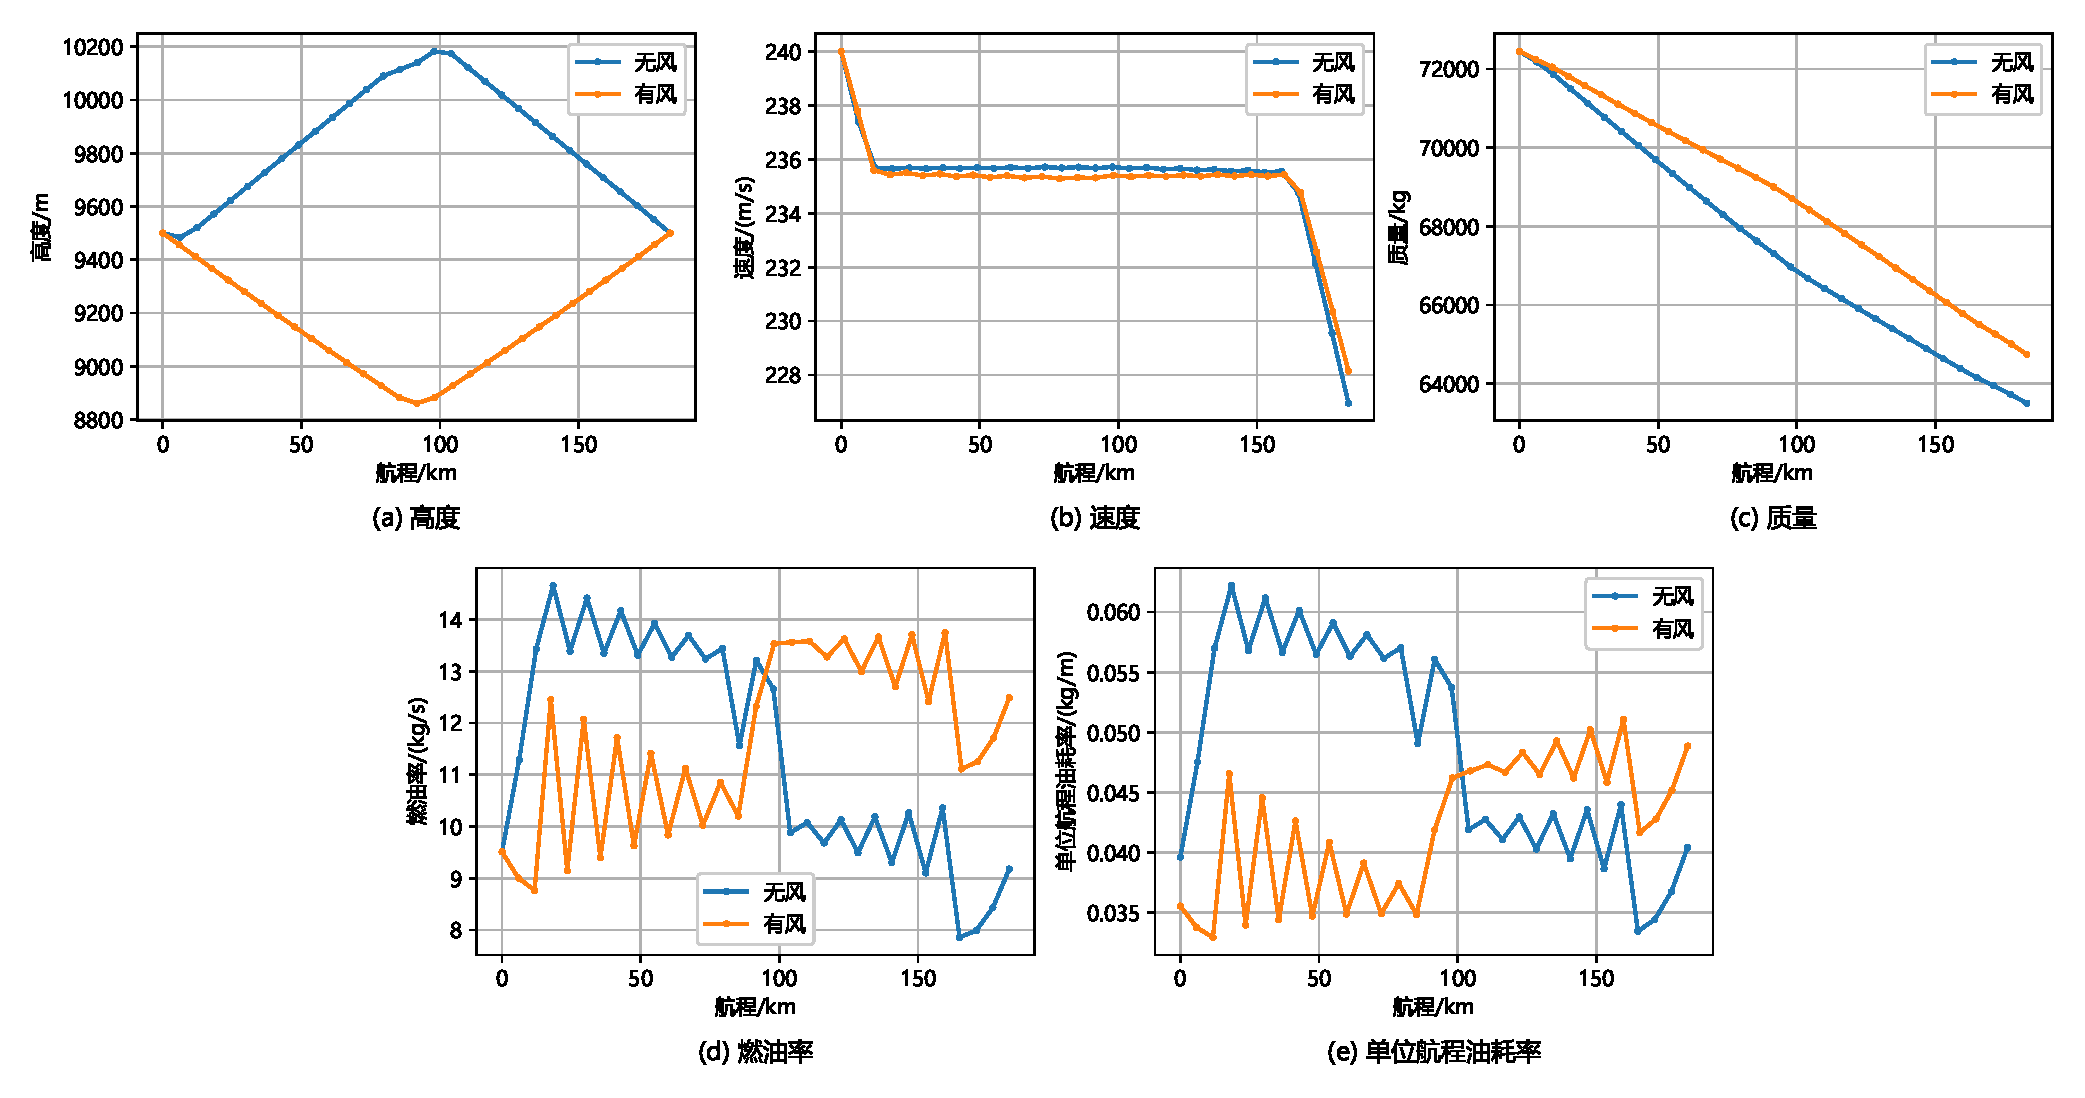
\includegraphics[width=0.9\textwidth]{6.eps}}{\fbox{Missing figure}}
	\caption{无风与有风条件下高度、速度、质量、燃油率和单位航程油耗率对比图}
	\label{fig:1}
\end{figure}

图 6 显示，无风条件下最优高度主要维持在 $9500\text{ m}$ 至 $10200\text{ m}$，有风条件下则整体略低，以利用较低高度层的顺风收益。两种工况下速度都基本保持在 $235\text{ m/s}$ 附近，说明速度偏离惩罚项有效约束了空速变化。燃油率和单位航程油耗率则随高度、速度和推力约束共同波动，但有风条件下前中段单位航程油耗率明显更低，因此终端质量更高、总油耗更少。

为验证数值解，本文采用直接法并结合 SLSQP 收敛性、配点残差和约束违背量进行检查，结果表明轨迹满足状态方程和约束，符合直接法意义下的 KKT 最优性条件。综上，时间域梯形配点法能够有效求解高度--速度联合最优巡航问题，有风最优轨迹的节油和节时优势主要来自地速提升和路径时间压缩。

\section{问题四模型建立与求解}
\subsection{模型建立}
\subsubsection{综合数值计算框架}
问题四需要在前三问模型基础上，建立完整的巡航策略综合数值计算模型。
本文采用统一的状态变量
\[
    \boldsymbol y(t)=\left[x(t),m(t),h(t),V(t)\right]^{\mathrm T},
\]
并采用问题三中的状态方程作为基本动力学约束。\

\subsubsection{等速巡航爬升策略模型}

等速巡航爬升策略中，空速保持为常数
\begin{equation}
    V(t)=V_c,
    \qquad
    \dot V(t)=0.
    \label{eq:q4_const_speed}
\end{equation}
其中，$V_c$ 可取初始空速 $V_0$ 或参考经济巡航速度 $V_{\mathrm{opt}}$。

为使飞机在质量逐渐减小的过程中保持合理的气动工作状态，本文令升力系数保持在初始巡航设计值
$C_{L,c}$ 附近。根据升力平衡关系，有
\begin{equation}
    C_{L,c}
    =
    \frac{2m(t)g}{\rho(h(t))V_c^2S}.
    \label{eq:q4_CL_const}
\end{equation}
若采用指数大气模型，则由式 (93) 可得到高度随质量变化的关系：
\begin{equation}
    h(t)
    =
    -H_\rho
    \ln
    \left[
    \frac{2m(t)g}{\rho_0V_c^2SC_{L,c}}
    \right].
    \label{eq:q4_h_m_const_speed}
\end{equation}
该式表明，随着燃油消耗导致飞机质量下降，为保持相同升力系数和固定空速，飞机应逐渐爬升至更高高度。

等速策略下的推力需求为
\begin{equation}
    F_{\mathrm{cs}}(t)
    =
    D_{\mathrm{cs}}(t)
    +
    \frac{m(t)g}{V_c}\dot h(t),
    \label{eq:q4_F_const_speed}
\end{equation}
其中，$D_{\mathrm{cs}}(t)$ 由对应高度、质量和速度下的阻力模型计算得到。
燃油消耗率为
\begin{equation}
    \phi_{\mathrm{cs}}(t)
    =
    c_fF_{\mathrm{cs}}(t)
    \left[
    1+\beta\left(V_c-V_{\mathrm{opt}}\right)^2
    \right].
    \label{eq:q4_phi_const_speed}
\end{equation}
相应状态方程为
\begin{equation}
\left\{
\begin{aligned}
    \dot x(t)&=V_c+W(h(t)),\\
    \dot m(t)&=-\phi_{\mathrm{cs}}(t).
\end{aligned}
\right.
\label{eq:q4_cs_ode}
\end{equation}
在初始条件 $x(0)=0,m(0)=m_0,h(0)=h_0$ 和终止质量 $m(t_f)=m_f$ 下，
数值积分式 (97) 即可得到等速策略下的高度、速度、质量和航程剖面。

\subsubsection{风场条件下的最优高度--速度联合轨迹模型}

考虑风场时，采用问题三建立的直接优化模型。若以固定终止质量 $m_f$ 为条件，
为了比较相同燃油消耗下的航程能力，可建立最大航程模型：
\begin{equation}
    \max_{\boldsymbol u(t),\,t_f}
    x(t_f),
    \label{eq:q4_range_objective}
\end{equation}
其约束为
\begin{equation}
\left\{
\begin{aligned}
    \dot x(t)&=V(t)+W(h(t)),\\
    \dot m(t)&=-\phi(t),\\
    \dot h(t)&=u_h(t),\\
    \dot V(t)&=u_V(t),
\end{aligned}
\right.
\label{eq:q4_opt_state}
\end{equation}
并满足
\begin{equation}
    x(0)=0,\quad m(0)=m_0,\quad h(0)=h_0,\quad V(0)=V_0,
    \label{eq:q4_opt_initial}
\end{equation}
\begin{equation}
    m(t_f)=m_f.
    \label{eq:q4_opt_terminal_mass}
\end{equation}
同时需满足高度、速度、马赫数、升力系数和推力约束。

若以等速策略得到的航程 $X_{\mathrm{cs}}$ 为固定航程，则可建立最小油耗模型：
\begin{equation}
    \min_{\boldsymbol u(t),\,t_f}
    J_{\mathrm{opt}}
    =
    \int_0^{t_f}\phi(t)\,\mathrm{d}t,
    \label{eq:q4_fuel_objective}
\end{equation}
其终止条件为
\begin{equation}
    x(t_f)=X_{\mathrm{cs}}.
    \label{eq:q4_fixed_range}
\end{equation}
通过上述两种等价比较方式，可以分别得到固定燃油条件下的航程提升和固定航程条件下的燃油节省。

\subsubsection{策略对比指标}

设等速策略的总燃油消耗量为 $J_{\mathrm{cs}}$，最优策略的总燃油消耗量为
$J_{\mathrm{opt}}$，则固定航程条件下的燃油节省比例定义为
\begin{equation}
    \eta_J
    =
    \frac{J_{\mathrm{cs}}-J_{\mathrm{opt}}}{J_{\mathrm{cs}}}\times 100\%.
    \label{eq:q4_fuel_saving}
\end{equation}

设等速策略在终止质量 $m_f$ 下的航程为 $X_{\mathrm{cs}}$，
最优策略在相同终止质量下的航程为 $X_{\mathrm{opt}}$，则航程提升比例定义为
\begin{equation}
    \eta_X
    =
    \frac{X_{\mathrm{opt}}-X_{\mathrm{cs}}}{X_{\mathrm{cs}}}\times 100\%.
    \label{eq:q4_range_improvement}
\end{equation}

\subsubsection{模型扩展一：温度偏差实时修正}

在实际飞行中，飞机可通过气象预报或机载传感器获得实时温度偏差信息。
将标准大气温度修正为
\begin{equation}
    T_{\mathrm{real}}(h,t)
    =
    T_{\mathrm{std}}(h)+\Delta T(h,t).
    \label{eq:q4_real_temperature}
\end{equation}
由此更新声速和密度：
\begin{equation}
    a_{\mathrm{real}}(h,t)
    =
    \sqrt{\gamma R_{\mathrm{gas}}T_{\mathrm{real}}(h,t)},
    \label{eq:q4_real_sound}
\end{equation}
\begin{equation}
    \rho_{\mathrm{real}}(h,t)
    \approx
    \rho(h)
    \left[
    1-\frac{\Delta T(h,t)}{T_{\mathrm{std}}(h)}
    \right].
    \label{eq:q4_real_density}
\end{equation}
将 $\rho_{\mathrm{real}}$ 和 $a_{\mathrm{real}}$ 分别代入阻力模型、升力约束和马赫数约束，
即可得到温度实时修正后的巡航优化模型。该扩展提高了模型对实际大气环境的适应能力，
但需要实时气象数据支持，并会增加数值求解过程中的参数更新成本。

\subsubsection{模型扩展二：发动机安装损失修正}

实际飞机发动机安装在机翼或机身上后，会受到进气畸变、短舱干扰和喷流干扰等影响，
使有效推力低于理想台架推力。为描述该影响，引入发动机安装效率 $\eta_{\mathrm{ins}}(h,V)$，
满足
\begin{equation}
    0<\eta_{\mathrm{ins}}(h,V)\leq 1.
    \label{eq:q4_eta_install}
\end{equation}
若 $F_{\mathrm{req}}(t)$ 为飞机完成当前飞行动作所需的有效推力，则发动机实际输出推力可表示为
\begin{equation}
    F_{\mathrm{cmd}}(t)
    =
    \frac{F_{\mathrm{req}}(t)}{\eta_{\mathrm{ins}}(h(t),V(t))}.
    \label{eq:q4_install_thrust}
\end{equation}
因此，考虑安装损失后的燃油消耗率修正为
\begin{equation}
    \phi_{\mathrm{ins}}(t)
    =
    c_fF_{\mathrm{cmd}}(t)
    \left[
    1+\beta\left(V(t)-V_{\mathrm{opt}}\right)^2
    \right].
    \label{eq:q4_install_fuel}
\end{equation}
同时，推力约束应修正为
\begin{equation}
    F_{\mathrm{req}}(t)
    \leq
    \eta_{\mathrm{ins}}(h(t),V(t))F_{\max}(h(t),V(t)).
    \label{eq:q4_install_constraint}
\end{equation}
该扩展使模型更接近真实发动机工作状态，但需要额外的发动机安装效率或推力包线数据。

\subsection{模型求解}
\subsubsection{等速巡航爬升基准策略求解}

根据式（92）—式（97），本文首先求解等速巡航爬升基准策略。计算中取 $V_c=V_0=240\text{ m/s}$，并以飞机质量由 $m_0=72450\text{ kg}$ 下降至 $m_f=62000\text{ kg}$ 作为积分终止条件。

在每一个离散时刻，先由式（94）根据当前质量计算对应飞行高度，再代入阻力模型、推力需求模型和燃油消耗率模型，得到当前推力需求和燃油消耗率。随后利用式（97）对质量和航程进行数值积分，得到等速巡航爬升策略下的高度、速度、质量、时间和航程剖面。

该策略作为问题四的基准方案。由于其终止质量固定为 $m_f$，所以基准燃油消耗量为 $J_{cs}=m_0-m_f=10450\text{ kg}$。数值积分得到基准航程为 $X_{cs}=200809.924516\text{ m}$。后续固定航程节油分析均以 $X_f=X_{cs}$ 为比较航程，固定燃油航程提升分析均以 $J_{cs}$ 为燃油上限。

\subsubsection{固定航程最小油耗模型求解}
为比较最优策略相对于等速策略的节油效果，本文首先采用固定航程比较方式。令最优策略完成与等速策略相同的航程，即取$X_f=X_{cs}.$

在该条件下，调用问题三建立的高度–速度联合最优控制模型，并以式（102）作为目标函数，以式（103）作为终端航程约束。数值求解时，采用问题三中的时间域梯形配点法，将连续最优控制问题转化为非线性规划问题。目标函数和状态方程分别按式（88）和式（89）离散。

在优化过程中，除满足状态方程外，还同时施加问题四建模部分给出的飞行安全边界、巡航运行约束和怠速推力约束。其中，怠速推力约束用于避免优化器通过过低推力或近似滑翔获得不符合实际巡航运行的低油耗结果。离散后的非线性规划问题采用 SLSQP 算法求解，并以最大约束违反量判断解的可行性。

本文取离散节点数为 $N=21$。优化器返回严格成功标志，且最大约束违反量为 $1.54845\times10^{-10}$，说明固定航程最优解满足数值可行性要求。
\subsubsection{固定燃油最大航程模型求解}
固定航程模型可以回答相同航程下的节油效果，但若只固定终止质量，则不同策略的总燃油消耗均接近 $m_0-m_f$，不适合直接比较节油比例。因此，本文进一步采用固定燃油最大航程模型，分析相同燃油消耗下最优策略的航程提升能力。

计算中以等速策略的燃油消耗量$J_{cs}=10450\text{ kg}$ 作为燃油上限。对于给定候选航程 $X$，重新求解高度–速度联合最优轨迹。若优化结果满足燃油消耗不超过 $J_{cs}$，且优化器返回严格可行解，则认为该候选航程可行。

搜索过程分为两步。首先从$1.2X_{cs}$ 开始进行外推搜索，逐步扩大候选航程，直到首次出现不可行解。随后在最后一个可行航程和第一个不可行航程之间进行二分搜索，得到固定燃油条件下的最大可行航程 $X_{opt}$。最终利用式（105）计算航程提升比例。
\subsubsection{模型扩展计算方法}
对于温度偏差实时修正扩展，本文在等速基准轨迹上选取离散样本点，计算每个节点处的$\Delta T(h,t)$、$T_{real}(h,t)$、$\rho_{real}(h,t)$ 和 $a_{real}(h,t)$。其中，修正后的密度进入升力系数、阻力和推力需求计算，修正后的声速进入马赫数计算。

对于发动机安装损失扩展，本文在同一组轨迹样本点上计算安装效率 $\eta_{ins}(h,V)$，并由式（110）和式（111）得到考虑安装损失后的发动机指令推力和燃油消耗率。该部分作为模型扩展框架的数值演示，用于说明新增因素进入原模型后的计算方式和影响方向。
\subsection{结果分析}
\subsubsection{等速策略与最优策略总体对比}
根据数值求解结果，等速巡航爬升策略在终止质量 $m_f=62000\text{ kg}$ 下的基准航程为 $200809.924516\text{ m}$，总燃油消耗为 $10450\text{ kg}$。

在固定相同航程 $X_f=X_{cs}$ 的条件下，考虑风场的高度–速度联合最优策略总油耗为 $8394.401214\text{ kg}$。由式（104）可得，固定航程下的燃油节省量为 $2055.598786\text{ kg}$，节油比例为 $19.670802\%$。

在固定燃油 $J_{cs}=10450\text{ kg}$的条件下，最优策略可达到的最大可行航程为 $256785.690975\text{ m}$。由式（105）可得，航程增加 $55975.766459\text{ m}$，航程提升比例为 $27.875000\%$。
\begin{table}[htbp]
\centering
\caption{问题四巡航策略综合对比}
\label{tab:comprehensive_comparison}
\begin{tabular}{cccccccc}
\toprule
 策略 & 总航程/km & 总油耗/kg & 终端高度/m  & 总时间/s \\
\midrule
 等速巡航爬升 & 200.81 & 10450 & 10637.1 & 762.454 \\
 固定航程最优策略 & 200.81 & 8394.4  & 9500 & 720.876 \\
 固定燃油最优策略 & 256.786 & 10446.7  & 9500 & 903.513 \\
\bottomrule
\end{tabular}
\end{table}

由表 6 可知，在完成相同航程时，最优策略能够以更少燃油到达终点，终端质量由等速策略的 $62000.0\text{ kg}$ 提高至 $64055.6\text{ kg}$。这说明优化节省的燃油直接表现为更高的终端剩余质量。在消耗近似相同燃油时，最优策略能够将航程由 $200.810\text{ km}$提高至 $256.786\text{ km}$，说明高度–速度联合优化能够显著提升单位燃油的航程效率。
\begin{figure}[H]
	\centering
	\IfFileExists{7.eps}{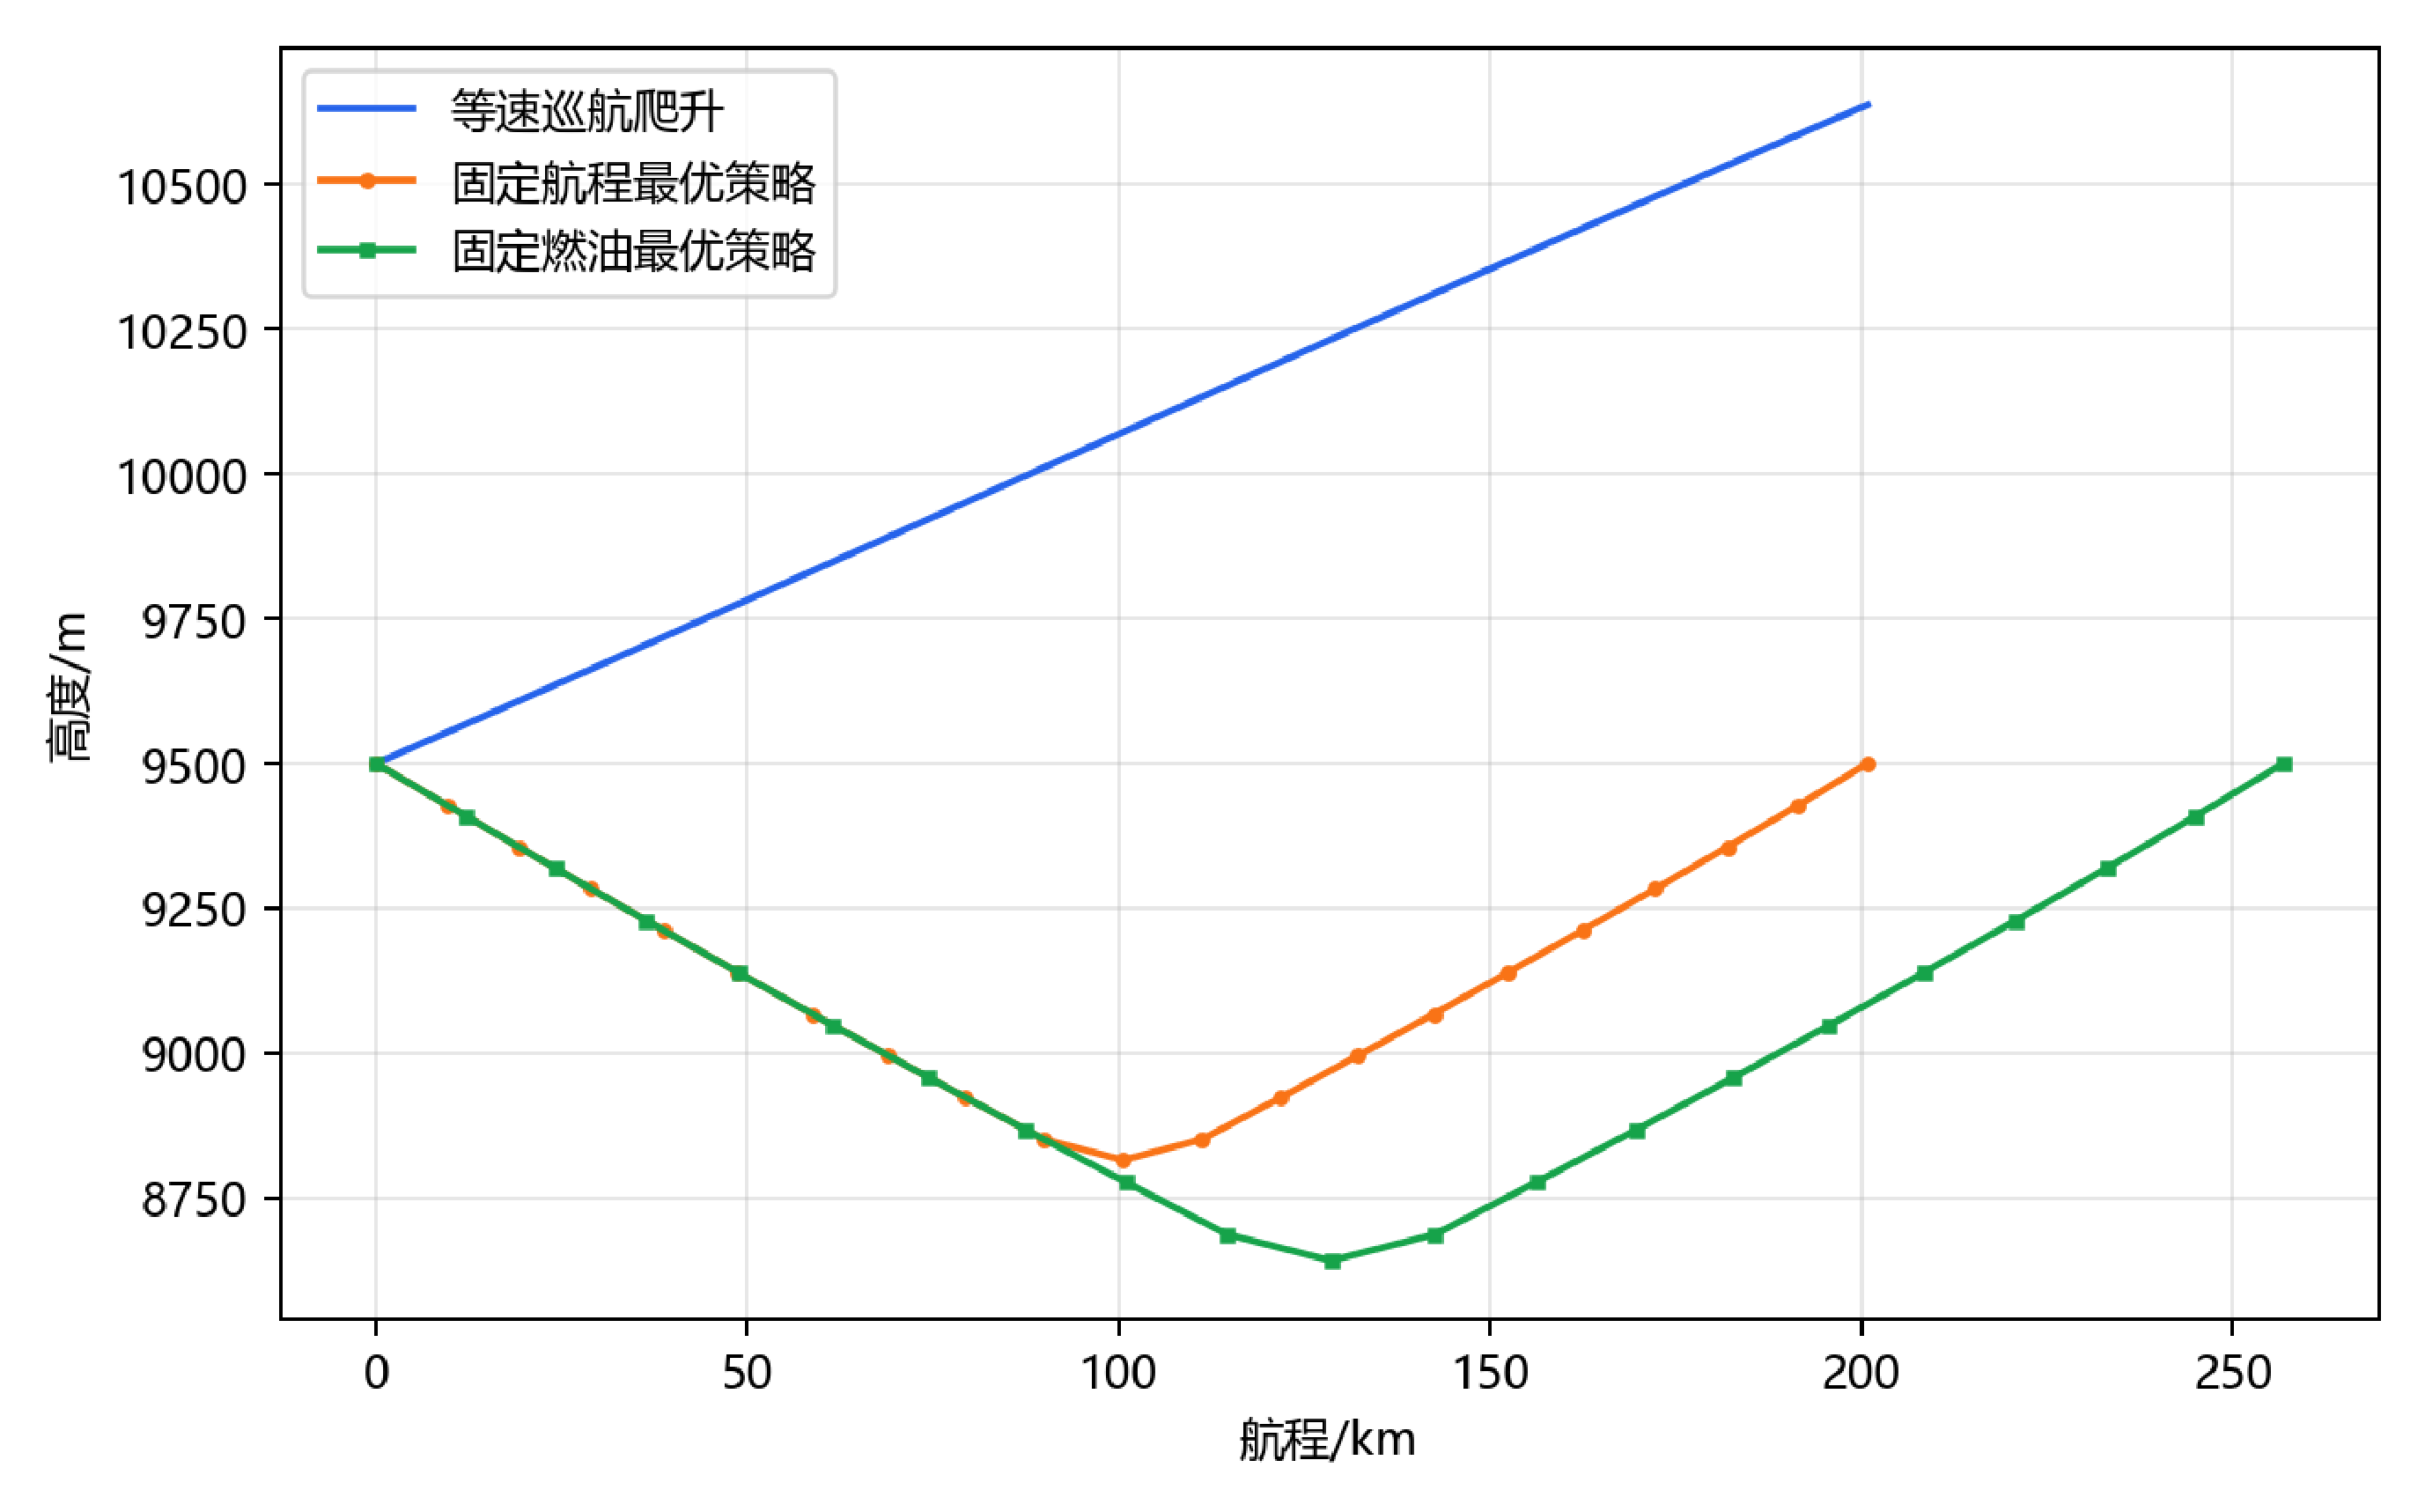
\includegraphics[width=0.6\textwidth]{7.eps}}{\fbox{Missing figure}}
	\caption{等速策略与最优策略高度剖面对比}
	\label{fig:2}
\end{figure}
由图7可知，等速巡航爬升策略随燃油消耗持续升高，最终高度达到约 $10637.1\text{ m}$；两类最优策略则先降低高度，再在后段回升到终端约束附近，说明最优轨迹是在风场收益、阻力变化和终端约束之间进行折中。

\subsubsection{最优高度–速度轨迹分析}
\begin{figure}[H]
	\centering
	\IfFileExists{8.eps}{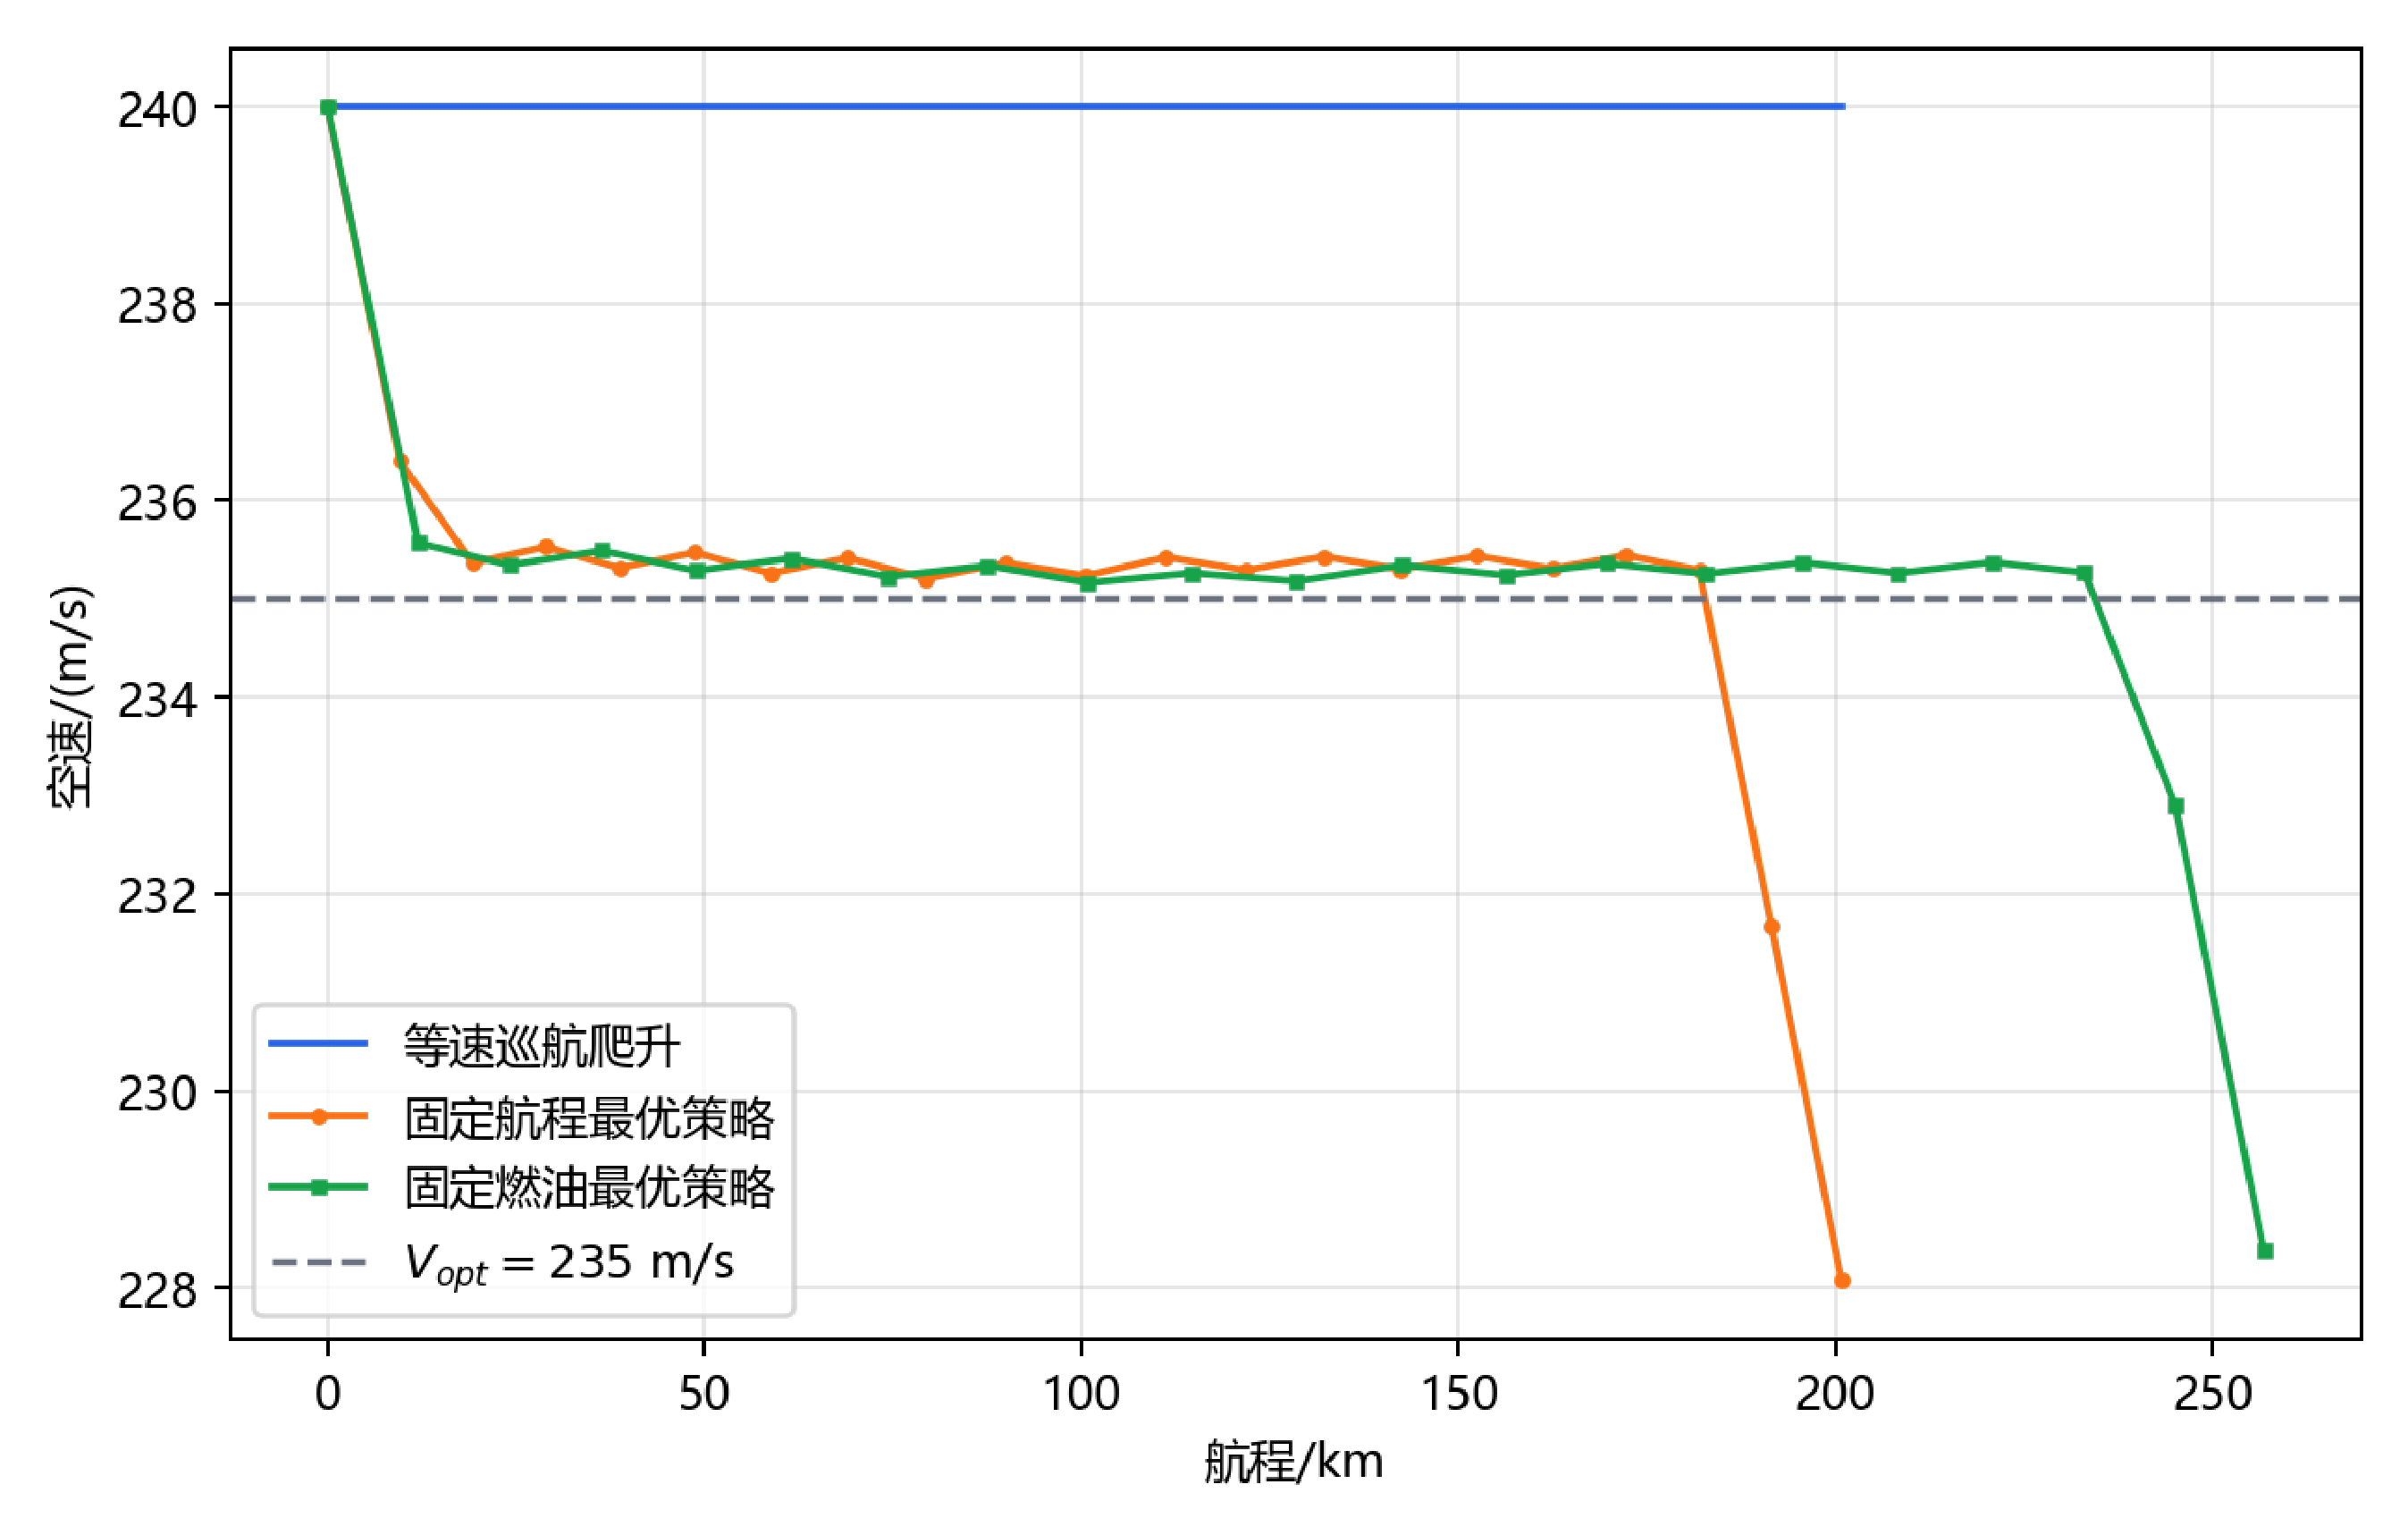
\includegraphics[width=0.6\textwidth]{8.eps}}{\fbox{Missing figure}}
    \caption{固定航程最优策略的高度、速度、质量与油耗率演化对比}
	\label{fig:3}
\end{figure}
固定航程最优策略的终端高度为 $9500.0\text{ m}$，正好落在高度下界，终端速度为 $228.080\text{ m/s}$，略高于速度下界 $225\text{ m/s}$。平均速度约为 $235\text{ m/s}$，接近参考经济速度 $V_{opt}=235\text{ m/s}$。这表明最优策略并不是单纯追求更高高度，而是在气动阻力、速度偏离损失和风场收益之间折中，并通过适度降速与局部降高提升单位航程效率。

\subsubsection{固定航程节油效果分析}
\begin{figure}[H]
	\centering
	\IfFileExists{9.eps}{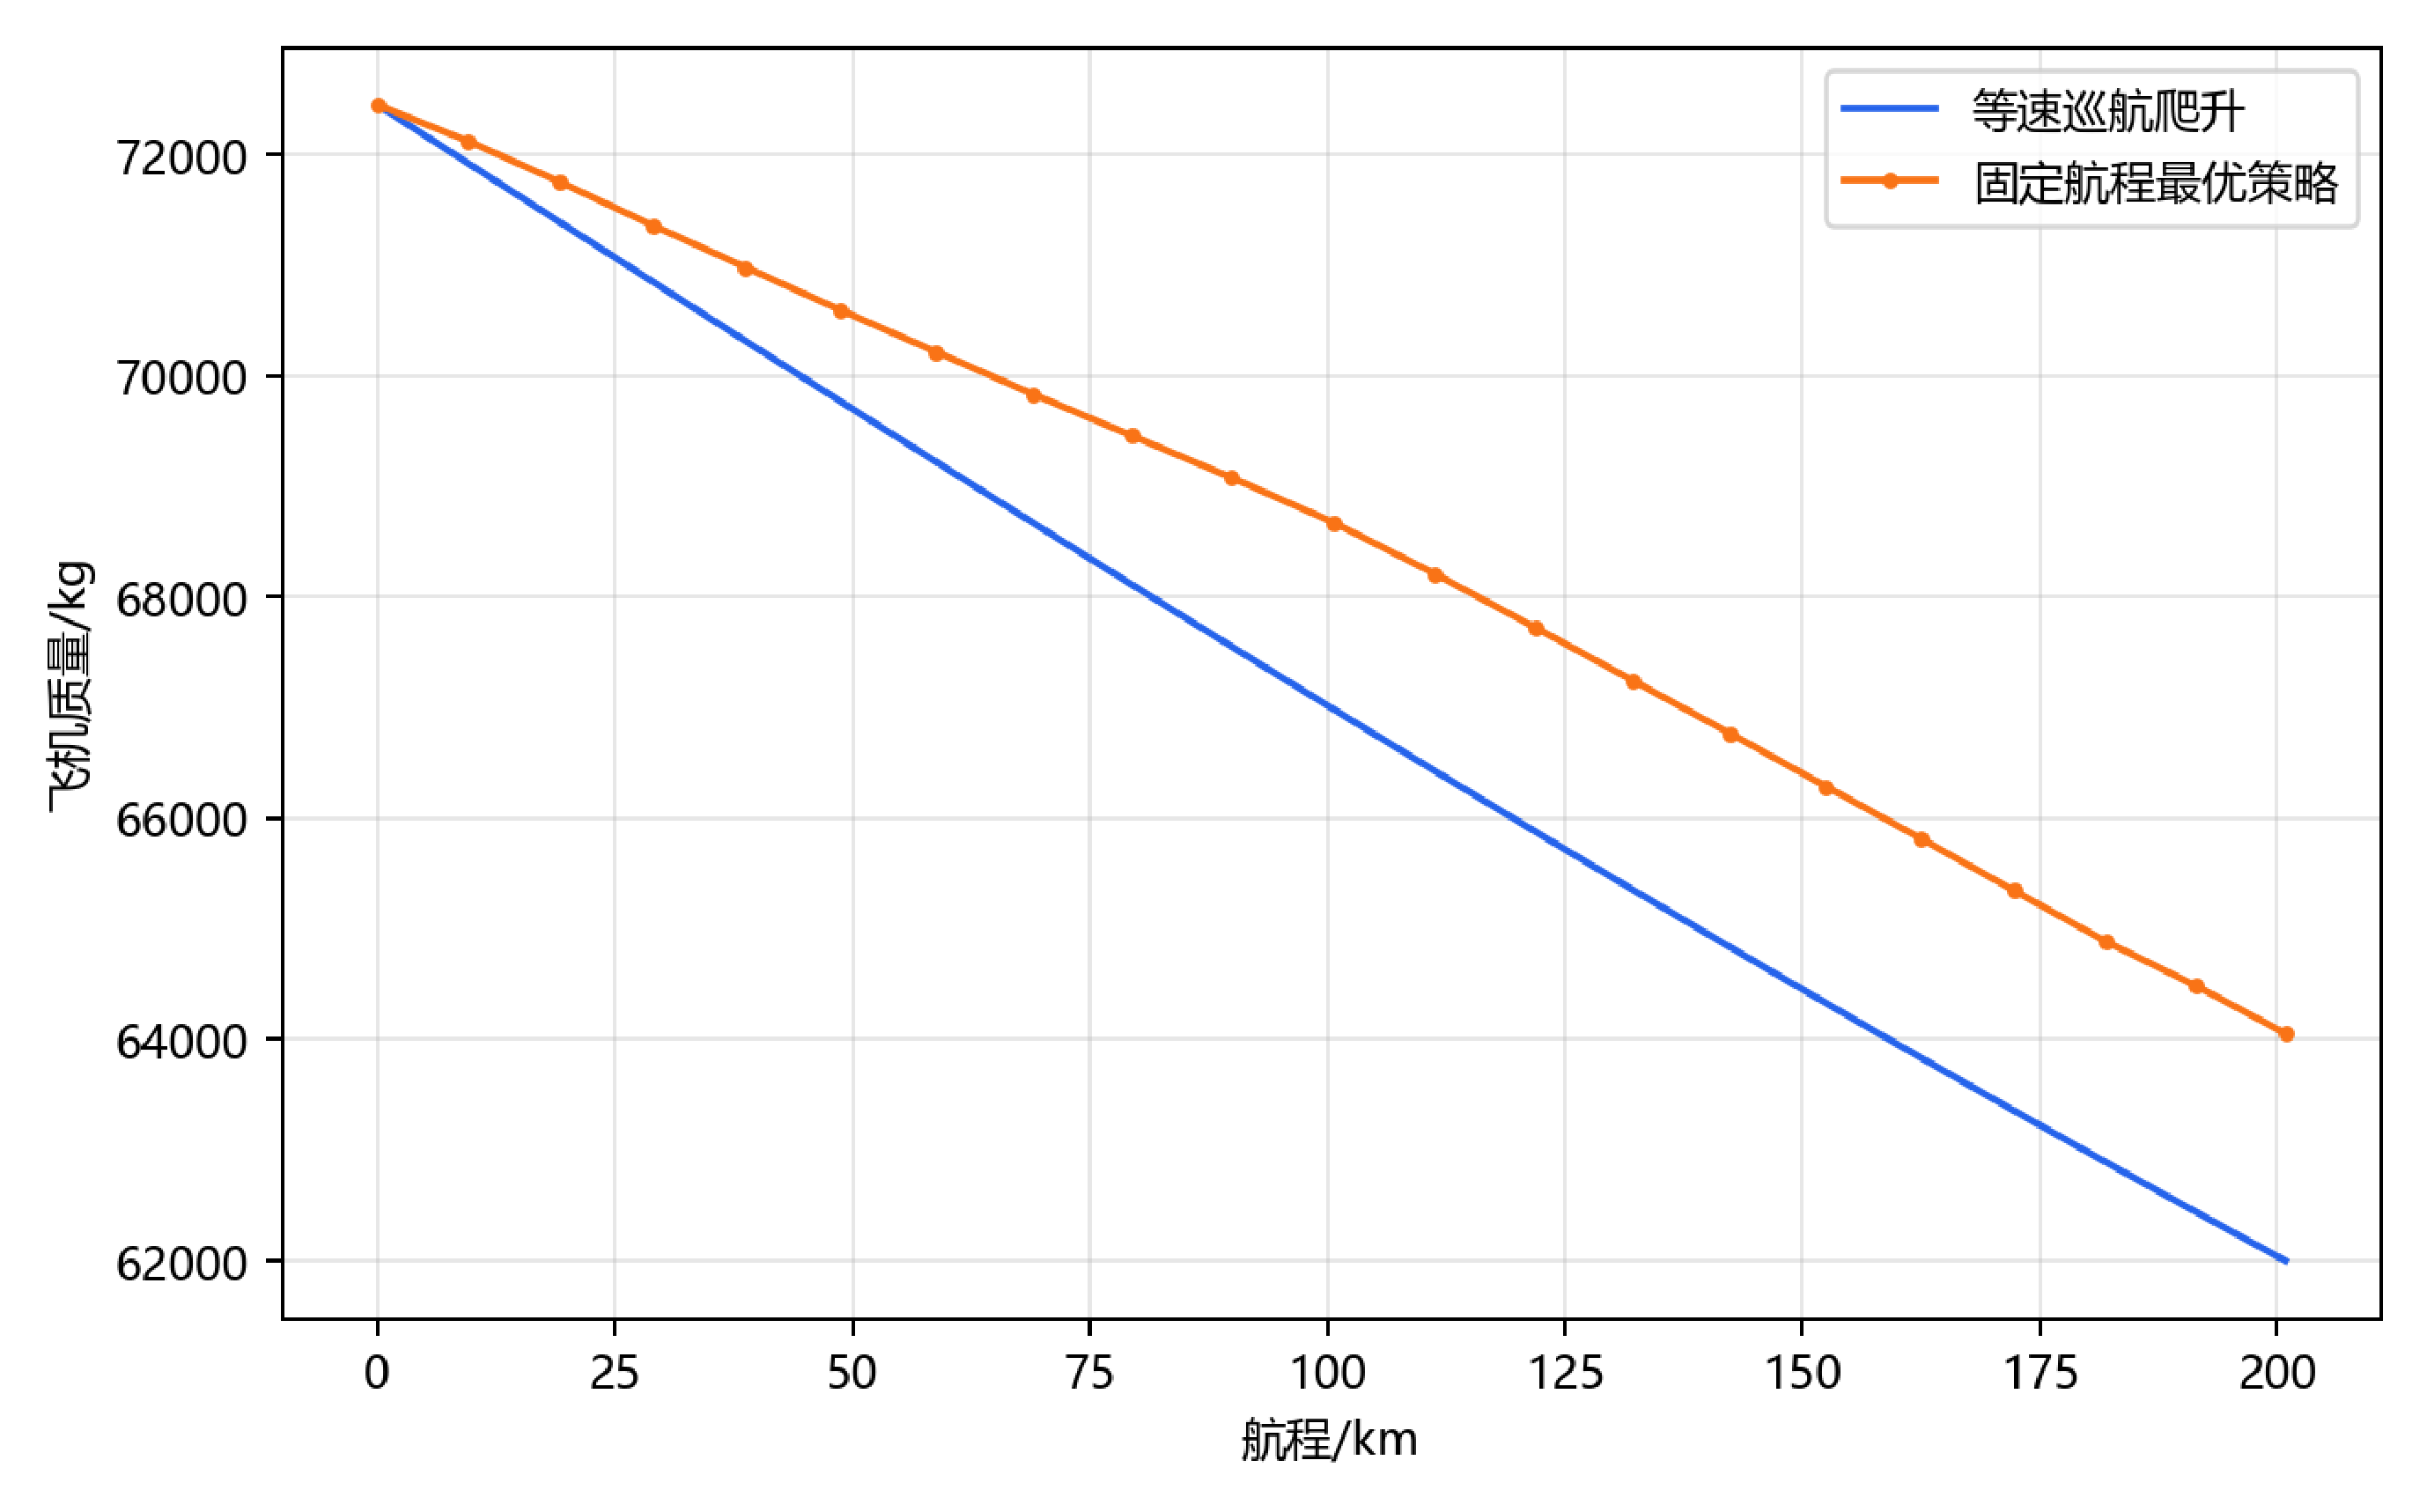
\includegraphics[width=0.6\textwidth]{9.eps}}{\fbox{Missing figure}}
    \caption{固定航程条件下等速策略与最优策略节油效果对比}
	\label{fig:4}
\end{figure}
固定航程下，等速策略完成 $200.810\text{ km}$ 需要 $10450.0\text{ kg}$ 燃油，而最优策略仅需 $8394.4\text{ kg}$，节油比例为 $19.670802\%$。节油主要来自三个方面：速度更接近 $V_{opt}$，风场带来更有利的地速，以及高度和速度的联合调节改善了阻力与爬升推力的平衡。

\subsubsection{固定燃油航程提升分析}
\begin{figure}[H]
	\centering
	\IfFileExists{10.eps}{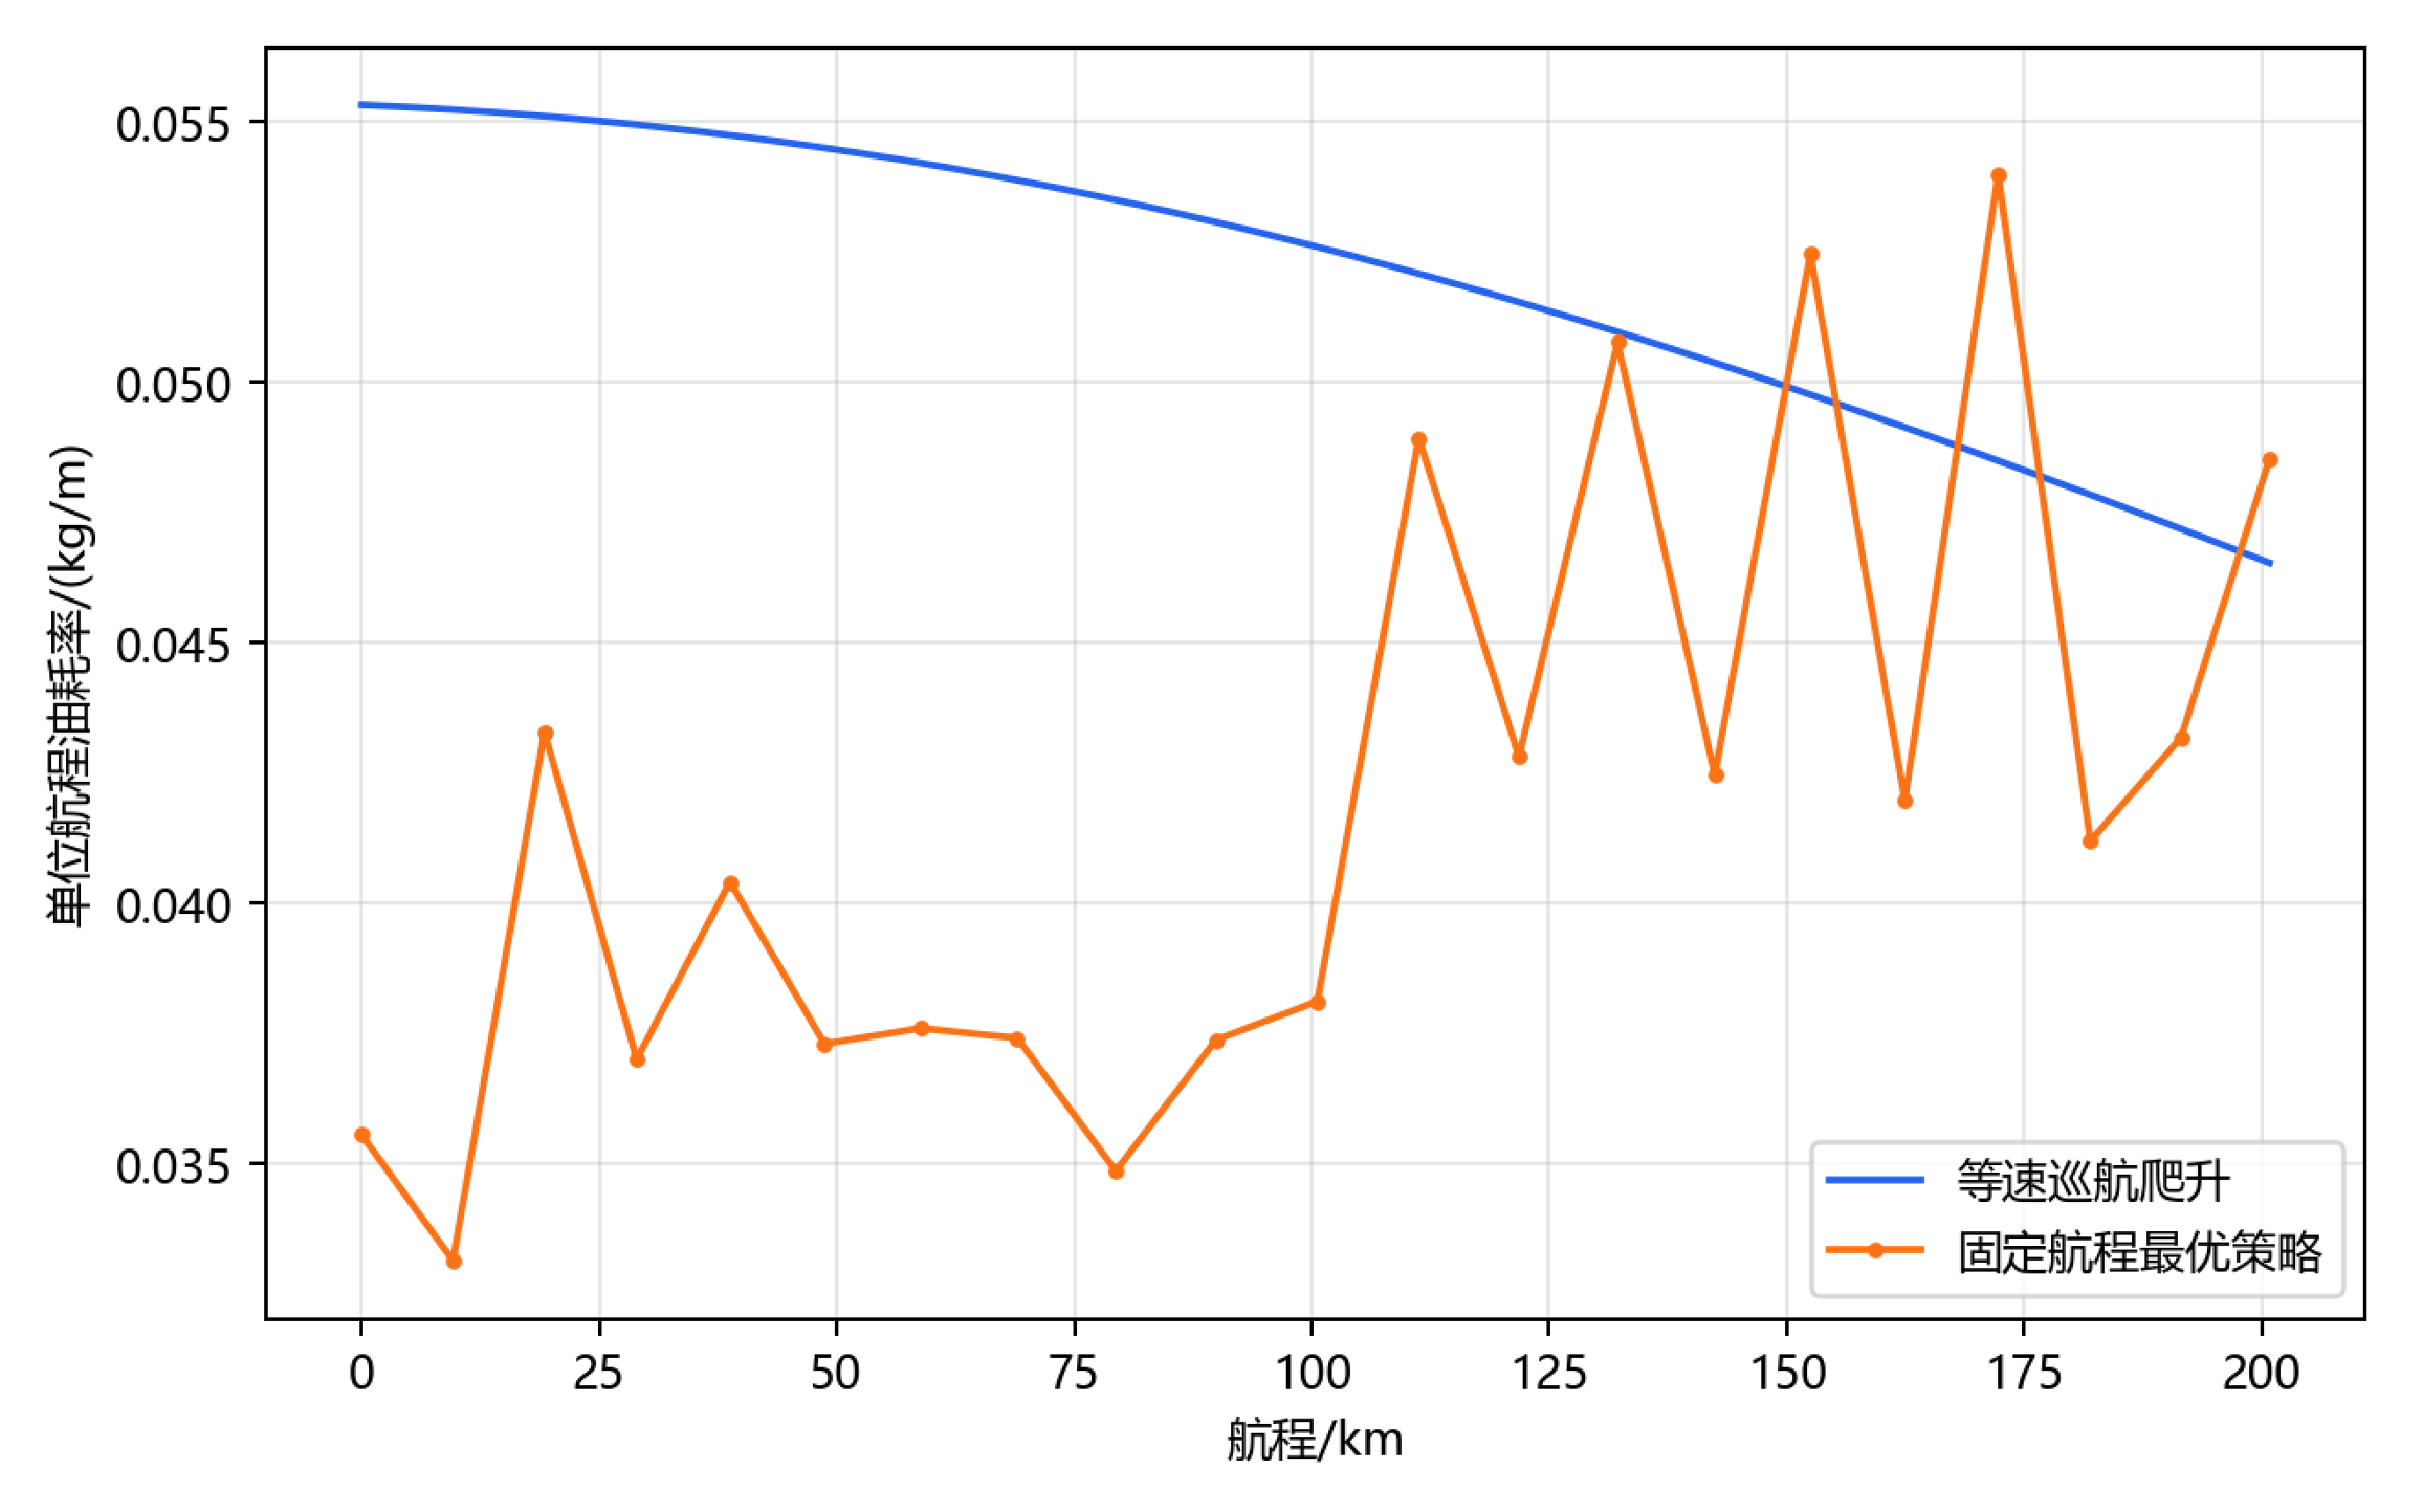
\includegraphics[width=0.6\textwidth]{10.eps}}{\fbox{Missing figure}}
    \caption{固定燃油条件下等速策略与最优策略航程提升对比}
	\label{fig:5}
\end{figure}
在燃油上限同为 $10450\text{ kg}$ 的条件下，最优策略最大可行航程为 $256.786\text{ km}$，比等速策略增加 $55.976\text{ km}$，航程提升比例为 $27.875000\%$。这说明高度–速度联合优化不仅能减少相同航程下的燃油消耗，也能在相同燃油储备下显著提升航程能力。
\subsubsection{模型扩展结果分析}
\begin{figure}[H]
	\centering
	\IfFileExists{11.eps}{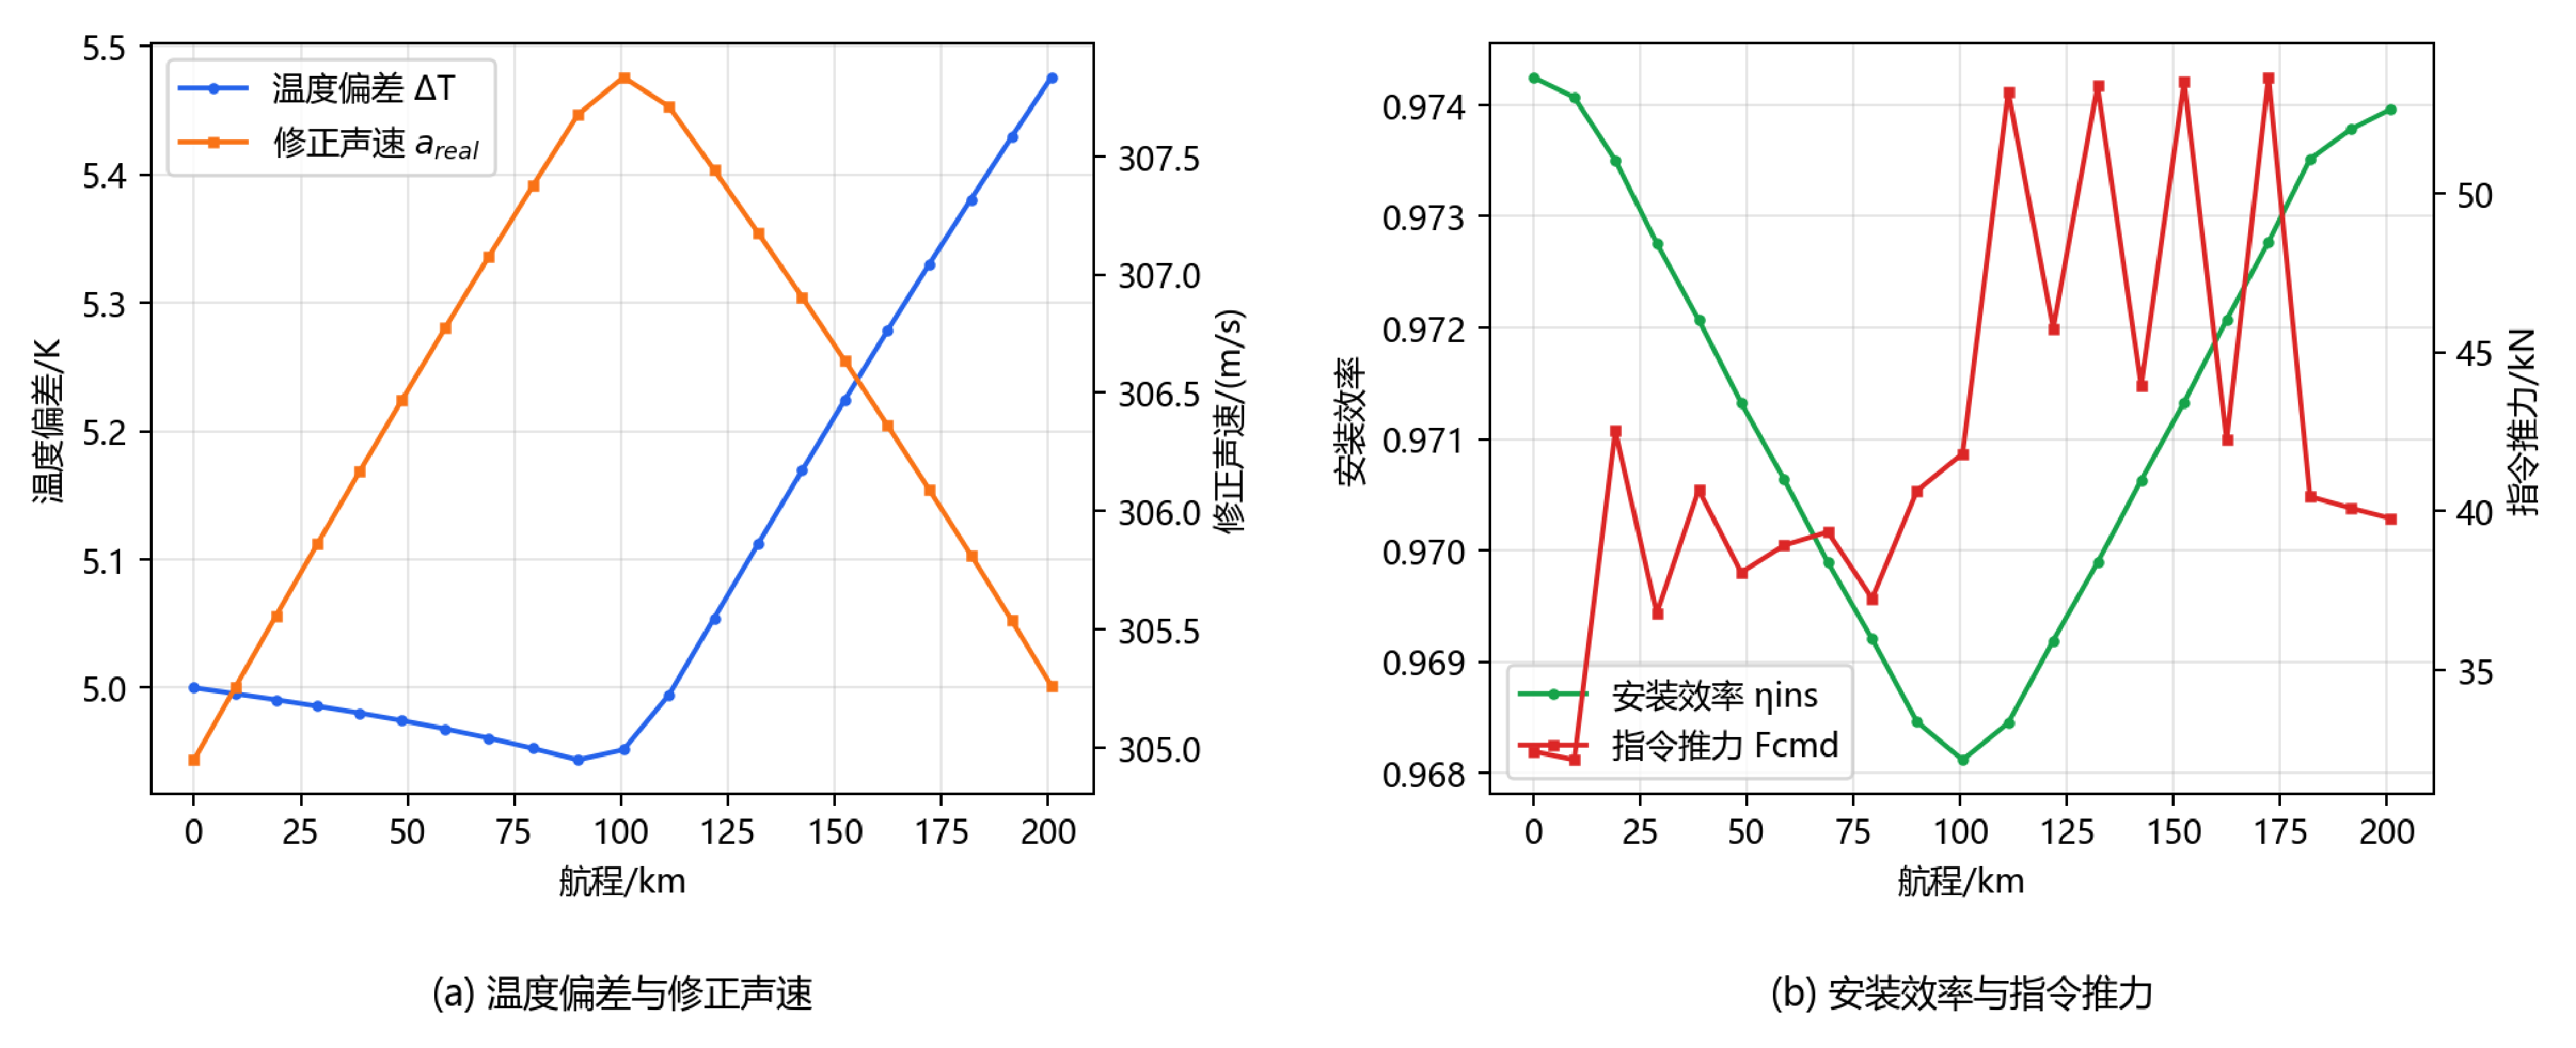
\includegraphics[width=1\textwidth]{11.eps}}{\fbox{Missing figure}}
	\caption{模型扩展参数沿航程变化}
	\label{fig:6}
\end{figure}
图 8-6 展示了温度偏差实时修正和发动机安装损失修正的数值效果。温度修正后，温度偏差与修正声速均随航程变化，说明大气参数不再只是单纯的高度函数，而是受高度和时间共同影响的非定常量。安装损失修正后，安装效率随航程波动，指令推力 $F_{cmd}$ 始终高于有效推力需求，反映出安装损失会放大发动机实际输出要求。

温度偏差扩展表明，密度和声速的同步修正会进一步影响升力系数、阻力、推力需求和马赫数约束；在等速基准轨迹的抽样计算中，温度偏差由初始约 $5.0\text{ K}$ 增至约 $6.04\text{ K}$，但模型结构保持不变，只是需要在每个离散节点更新 $T_{real}$、$\rho_{real}$ 和 $a_{real}$。安装损失扩展则表明，考虑 $\eta_{ins}(h,V)$ 后，初始时刻安装效率约为 $0.97425$，所需有效推力约为 $49172.3\text{ N}$，修正后的指令推力约为 $50472.0\text{ N}$，因此燃油消耗会进一步增加。

总体来看，这两个扩展都没有改变原模型的主框架，但分别通过大气参数和推力需求引入了额外的非线性。若进一步加入最大推力包线，则工程真实性会更强，但也需要更多安装效率和推力包线数据支撑。

\section{灵敏度分析} 

\subsubsection{速度偏离惩罚系数敏感性分析}

速度偏离惩罚系数 $\beta$ 刻画了空速偏离最佳效率速度后燃油消耗增加的强度。
为分析模型对该参数的敏感性，令
\begin{equation}
    \beta_{\alpha}=\alpha\beta_0,
    \label{eq:q4_beta_alpha}
\end{equation}
其中，$\beta_0$ 为题目给定的标称值，$\alpha$ 为扰动系数，可取
$\alpha\in\{0.8,0.9,1.0,1.1,1.2\}$。

对于每一个 $\beta_{\alpha}$，重新求解最优巡航轨迹，得到对应的最优目标函数值
$J^*(\beta_{\alpha})$、最优高度轨迹 $h^*(t;\beta_{\alpha})$ 和最优速度轨迹
$V^*(t;\beta_{\alpha})$。定义目标函数对 $\beta$ 的相对敏感度为
\begin{equation}
    S_J
    =
    \frac{
    J^*(\beta_0(1+\varepsilon))-J^*(\beta_0(1-\varepsilon))
    }{
    2\varepsilon J^*(\beta_0)
    },
    \label{eq:q4_sensitivity_J}
\end{equation}
其中，$\varepsilon$ 为小扰动比例。类似地，可定义最终高度、平均速度和总航程等指标的敏感度，
从而识别模型中对速度惩罚系数变化最敏感的环节。
\begin{table}[ht]
\centering
\caption{速度偏离惩罚系数敏感性分析}
\label{tab:sensitivity_penalty}
\begin{tabular}{ccccccc}
\toprule
$\lambda_{\alpha}$ & $\lambda_{\beta}$ & 最优油耗/kg & 节油比例/\%  & 终端速度/(m/s) & 平均速度/(m/s) \\
\midrule
0.8   & 0.0024 & 8382.1  & 19.7885 & 227.456 & 235.086 \\
0.9   & 0.0027 & 8388.55 & 19.7268 & 227.801 & 235.097 \\
1.0   & 0.0030 & 8394.4  & 19.6708 & 228.079 & 235.104 \\
1.1   & 0.0033 & 8399.7  & 19.6201 & 228.466 & 235.117 \\
1.2   & 0.0036 & 8404.41 & 19.5750 & 228.801 & 235.129 \\
\bottomrule
\end{tabular}
\end{table}

由表 6 可知，随着 $\beta$增大，最优油耗由 $8382.10\text{ kg}$ 增加至 $48404.41\text{ kg}$，节油比例由 $19.7885\%$ 降低至 $19.5750\%$。该趋势符合速度偏离惩罚项的物理意义：当速度偏离经济速度的代价增大时，优化器在速度调节上的自由度下降，可获得的燃油节省略有减少。

同时，虽然 $\beta$ 变化幅度达到 $\pm 20\%$，但最优油耗变化仅约 $22.31\text{ kg}$，相对于基准油耗 $10450\text{ kg}$ 的比例较小。所有扰动情形下，节油比例均保持在 $19.5\%$ 以上，说明高度–速度联合优化的优势并不依赖某一个特定的 $\beta$ 取值，而是在标称值附近具有较好的稳定性。
\begin{figure}[H]
	\centering
	\IfFileExists{12.eps}{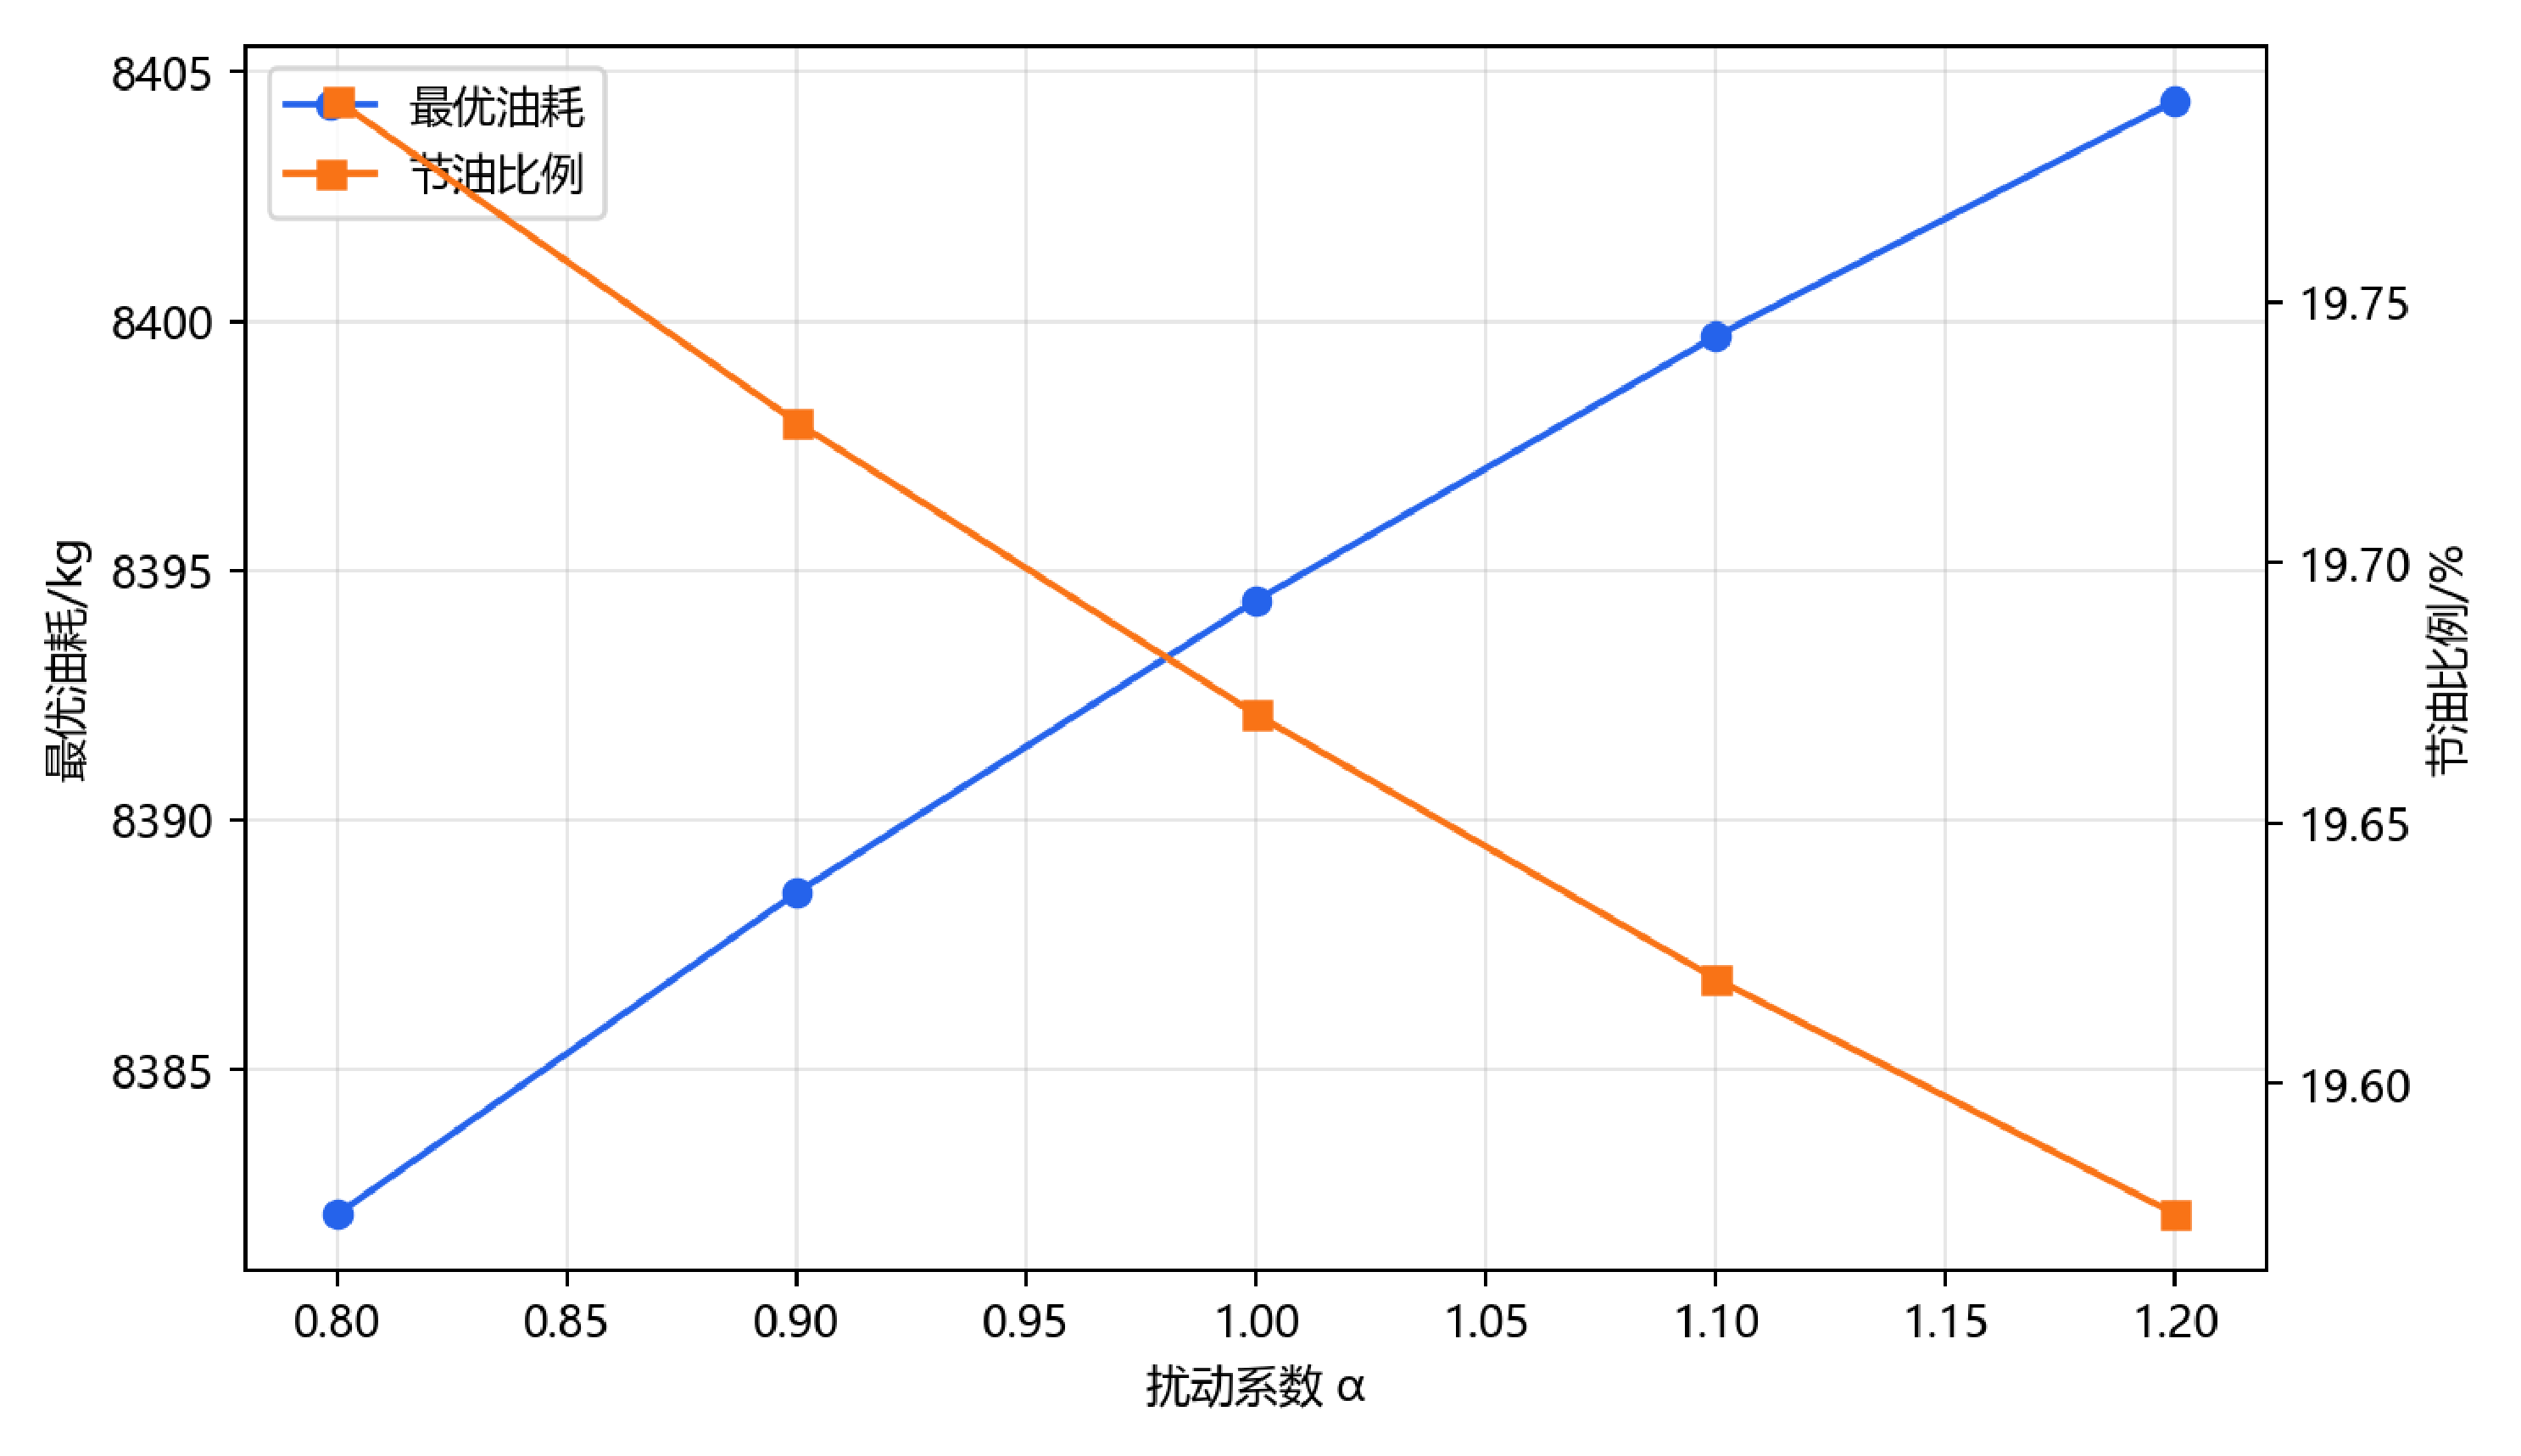
\includegraphics[width=0.7\textwidth]{12.eps}}{\fbox{Missing figure}}
	\caption{模型扩展参数沿航程变化}
	\label{fig:7}
\end{figure}
图 12 进一步给出了不同 $\beta$ 取值下的最优空速轨迹。各曲线在大部分航段均围绕 $V_{opt}=235\text{ m/s}$ 小幅波动，说明经济速度对最优空速具有稳定吸引作用。随着$\alpha$ 增大，末端空速略有提高，但整体轨迹差异不大，进一步说明速度偏离惩罚系数在标称值附近变化时不会明显改变最优轨迹结构。

从轨迹结构看，不同 $\beta$ 下的终端高度均为 $9500\text{ m}$，说明终端高度约束对最优解具有较强限制作用。平均速度始终维持在 $235\text{ m/s}$ 附近，说明参考经济速度 $V_{opt}$ 对速度轨迹具有明显约束作用。随着 $\beta$ 增大，终端速度由 $227.456\text{ m/s}$ 增至 $228.801\text{ m/s}$，速度轨迹整体略向更平稳、更接近经济速度的方向调整。
\newpage
%Reference
\begin{thebibliography}{40}
	\bibitem{1}Delgado Muñoz, L., \& Prats Menéndez, X. (2009). Fuel consumption assessment for speed variation concepts during the cruise phase. In Conference on Air Traffic Management Economics.
	\bibitem{2}Atmosphere, U. S. (1976). US Government Printing Office: Washington. DC, USA, 1-241.
    \bibitem{3}王兵, 张博雯, \& 彭瑛. (2025). 基于历史航迹数据的民用航空器极曲线估算方法. 交通运输工程学报, 25(4), 328-339.
	\bibitem{4}Valenzuela Romero, A., \& Rivas Rivas, D. (2014). Analysis of Wind-Shear Effects on Optimal Aircraft Cruise. International Conference on Research in Air Transportation (ICRAT).
    \bibitem{5}Anderson Jr, J. D. (1991). Fundamentals of Aerodynamics, McGraw-Hill. New York.
    \bibitem{6}陈兴荣. (1988). 飞机颠簸的气象因素分析. 中国民航学院学报(综合版), (3), 36-45.
    \bibitem{7}吴慰祖. (1989). 飞机全尺寸阻力的预计. 飞行力学, (3), 11-27. https://doi.org/10.13645/j.cnki.f.d.1989.03.002
    \bibitem{8}Tyrén, C. (1982). Magnetic anomalies as a reference for ground-speed and map-matching navigation. The Journal of navigation, 35(2), 242-254.
    \bibitem{9}Filippone, A. (2012). Advanced aircraft flight performance (Vol. 34). Cambridge University Press.
    \bibitem{10}Torenbeek, E. (2013). Unified Cruise Performance.
    \bibitem{11}吴奕铭.(2022).运输类飞机商业飞行的性能分析规范及实例研究(硕士学位论文,中国民用航空飞行学院).硕士https://doi.org/10.27722/d.cnki.gzgmh.2022.000286.
    \bibitem{12}高浩.(1984).改善乘坐品质纵向增稳器返馈系数的选择.航空学报,(1),18-23.
\end{thebibliography}
\newpage
\newgeometry{left=1.50cm,right=0.5cm,top=3.00cm,bottom=3.0cm}	%修改附录代码的几何页面

\begin{center}
	\sihao \heiti 附录
	
	
	\fontsize{10pt}{16pt}		\selectfont	
	\begin{lstlisting}[ language=MATLAB,numbers=left,numberstyle=\tiny,keywordstyle=\color{blue!70},commentstyle=\color{red!50!green!50!blue!50},frame=shadowbox, rulesepcolor=\color{red!20!green!20!blue!20},escapeinside=||,xleftmargin=2em,xrightmargin=2em,aboveskip=1em] 
	%%%问题一
	from __future__ import annotations

import sys
from pathlib import Path

import matplotlib

matplotlib.use("Agg")
import matplotlib.pyplot as plt
import numpy as np
import pandas as pd
from scipy.optimize import brentq

ROOT = Path(__file__).resolve().parents[1]
if str(ROOT) not in sys.path:
    sys.path.insert(0, str(ROOT))

from common.aerodynamics import drag, lift_coefficient
from common.atmosphere import T_std, mach_number, sound_speed, wind_for_mode
from common.fuel_model import speed_penalty
from common.parameters import PARAMS, Parameters
from common.utils import (
    cumulative_trapezoid_from_values,
    ensure_dir,
    save_dataframe,
    save_figure,
)


def compute_constant_speed_profile(
    n_points: int = 1200,
    wind_mode: str = "strict",
    params: Parameters = PARAMS,
) -> pd.DataFrame:
    """Constant-air-speed cruise-climb profile integrated over mass."""
    mass = np.linspace(params.m0, params.mf, n_points)
    fuel_used = params.m0 - mass
    V = np.full_like(mass, params.V0)

    # Constant CL gives h = h0 - Hrho*ln(m/m0).
    CL_c = lift_coefficient(params.m0, params.h0, params.V0, params)
    h = params.h0 - params.Hrho * np.log(mass / params.m0)

    D = drag(mass, h, V, params)
    penalty = speed_penalty(V, params)
    p = params.cF * penalty
    coupling = params.Hrho * params.g / params.V0
    denom = 1.0 - p * coupling
    if np.any(denom <= 0):
        raise RuntimeError("Constant-speed fuel-rate coupling denominator is non-positive.")
    rate = p * D / denom
    hdot = params.Hrho * rate / mass
    thrust = rate / p
    CL = lift_coefficient(mass, h, V, params)
    mach = mach_number(V, h, params)
    W = wind_for_mode(h, wind_mode)
    ground_speed = V + W

    time_s = cumulative_trapezoid_from_values(1.0 / rate, fuel_used)
    distance_m = cumulative_trapezoid_from_values(ground_speed / rate, fuel_used)

    return pd.DataFrame(
        {
            "time_s": time_s,
            "height_m": h,
            "mass_kg": mass,
            "velocity_mps": V,
            "mach": mach,
            "lift_coefficient": CL,
            "reference_lift_coefficient": CL_c,
            "drag_N": D,
            "thrust_N": thrust,
            "fuel_rate_kgps": rate,
            "climb_rate_mps": hdot,
            "wind_mps": W,
            "ground_speed_mps": ground_speed,
            "distance_m": distance_m,
            "fuel_used_kg": fuel_used,
        }
    )


def _constant_mach_height_from_mass(mass: float, params: Parameters) -> float:
    T_ref = T_std(params.h0, params)
    target = mass / params.m0

    def relation(h):
        return np.exp(-(h - params.h0) / params.Hrho) * T_std(h, params) / T_ref - target

    if abs(mass - params.m0) < 1e-10:
        return params.h0
    return brentq(relation, params.h0, 20000.0, xtol=1e-10, rtol=1e-10)


def compute_constant_mach_profile(
    n_points: int = 1200,
    wind_mode: str = "strict",
    params: Parameters = PARAMS,
) -> pd.DataFrame:
    """Constant-Mach cruise-climb profile integrated over mass."""
    mass = np.linspace(params.m0, params.mf, n_points)
    fuel_used = params.m0 - mass
    M0 = params.V0 / sound_speed(params.h0, params)
    h = np.array([_constant_mach_height_from_mass(m, params) for m in mass])
    T = T_std(h, params)
    V = M0 * sound_speed(h, params)

    D = drag(mass, h, V, params)
    penalty = speed_penalty(V, params)
    p = params.cF * penalty

    # Differentiate ln(m/m0) = -(h-h0)/Hrho + ln(T/T0h).
    A = -1.0 / params.Hrho - params.LT / T
    B = -1.0 / (mass * A)  # hdot = B*fuel_rate
    dVdh = -V * params.LT / (2.0 * T)
    denom = 1.0 - p * mass * B * (dVdh + params.g / V)
    if np.any(denom <= 0):
        raise RuntimeError("Constant-Mach fuel-rate coupling denominator is non-positive.")
    rate = p * D / denom
    hdot = B * rate
    Vdot = dVdh * hdot
    thrust = rate / p
    CL = lift_coefficient(mass, h, V, params)
    mach = mach_number(V, h, params)
    W = wind_for_mode(h, wind_mode)
    ground_speed = V + W

    time_s = cumulative_trapezoid_from_values(1.0 / rate, fuel_used)
    distance_m = cumulative_trapezoid_from_values(ground_speed / rate, fuel_used)

    return pd.DataFrame(
        {
            "time_s": time_s,
            "height_m": h,
            "mass_kg": mass,
            "velocity_mps": V,
            "mach": mach,
            "lift_coefficient": CL,
            "drag_N": D,
            "thrust_N": thrust,
            "fuel_rate_kgps": rate,
            "climb_rate_mps": hdot,
            "acceleration_mps2": Vdot,
            "wind_mps": W,
            "ground_speed_mps": ground_speed,
            "distance_m": distance_m,
            "fuel_used_kg": fuel_used,
        }
    )


def build_summary(cs: pd.DataFrame, cm: pd.DataFrame, params: Parameters = PARAMS) -> pd.DataFrame:
    rows = []
    for strategy, df in [
        ("constant_speed", cs),
        ("constant_mach", cm),
    ]:
        total_time = float(df["time_s"].iloc[-1])
        final_height = float(df["height_m"].iloc[-1])
        rows.append(
            {
                "strategy": strategy,
                "final_height_m": final_height,
                "total_time_s": total_time,
                "total_time_min": total_time / 60.0,
                "final_distance_m": float(df["distance_m"].iloc[-1]),
                "final_distance_km": float(df["distance_m"].iloc[-1]) / 1000.0,
                "fuel_consumption_kg": params.m0 - params.mf,
                "average_climb_rate_mps": (final_height - params.h0) / total_time,
            }
        )
    return pd.DataFrame(rows)


def make_figures(cs: pd.DataFrame, cm: pd.DataFrame, figures_dir: Path):
    ensure_dir(figures_dir)
    plt.rcParams["font.sans-serif"] = [
        "Microsoft YaHei",
        "SimHei",
        "Noto Sans CJK SC",
        "Arial Unicode MS",
        "DejaVu Sans",
    ]
    plt.rcParams["axes.unicode_minus"] = False
    datasets = [("等速策略", cs), ("等马赫策略", cm)]

    def line_plot(filename, y_col, y_label):
        fig, ax = plt.subplots(figsize=(8, 5))
        for label, df in datasets:
            ax.plot(df["time_s"] / 60.0, df[y_col], label=label)
        ax.set_xlabel("时间/min")
        ax.set_ylabel(y_label)
        ax.grid(True, alpha=0.3)
        ax.legend()
        save_figure(figures_dir / filename, fig)

    line_plot("height_vs_time.png", "height_m", "高度/m")
    line_plot("mass_vs_time.png", "mass_kg", "质量/kg")
    line_plot("climb_rate_vs_time.png", "climb_rate_mps", "爬升率/(m/s)")


def write_explanation(summary: pd.DataFrame, path: Path):
    cs = summary.loc[summary["strategy"] == "constant_speed"].iloc[0]
    cm = summary.loc[summary["strategy"] == "constant_mach"].iloc[0]
    content = f"""# 问题 1 数值说明

## 求解目标


## 数学模型

`F = D + m Vdot + m g hdot / V`

等马赫策略固定 `M0=V0/a(h0)`，速度随高度由 `V(h)=M0 a(h)` 给出，高度由隐式关系

`m/m0 = exp(-(h-h0)/Hrho) T(h)/T(h0)`

用 `scipy.optimize.brentq` 逐点求解。

## 输出文件
·
- `problem1_constant_speed_profile.csv`：等速策略完整剖面。
- `problem1_constant_mach_profile.csv`：等马赫数策略完整剖面。
- `problem1_summary.csv`：两种策略终值与总量对比。
- `height_vs_time.png`、`mass_vs_time.png` 和 `climb_rate_vs_time.png`：剖面图。

## 关键结果

- 等速策略最终高度为 {cs['final_height_m']:.3f} m，总时间为 {cs['total_time_min']:.3f} min，按默认题面风场计算的航程为 {cs['final_distance_km']:.3f} km。
- 等马赫策略最终高度为 {cm['final_height_m']:.3f} m，总时间为 {cm['total_time_min']:.3f} min，按默认题面风场计算的航程为 {cm['final_distance_km']:.3f} km。
- 两种策略燃油消耗均为从 `m0` 到 `mf` 的质量差，即 {cs['fuel_consumption_kg']:.3f} kg。

等速策略通过保持参考升力系数使高度随质量下降逐渐升高。等马赫数策略中声速随标准大气温度降低而减小，因此空速会随爬升略降；其爬升率大小取决于阻力、速度惩罚和隐式高度-质量关系的共同作用，不能强行固定为一定大于等速策略。

## 风场数量级提醒

代码默认使用修正后的风场 `W(h)=20+3*10^(-5)(h-10000)^2`。在 9500 m 附近该式给出约 27.5 m/s 的风速，数量级比原先 `0.003` 系数下的结果合理得多。公共函数中仍保留 `capped` 与 `scaled` 模式，便于后续做稳健性检查。
"""
    path.write_text(content, encoding="utf-8")
    print(f"Saved explanation: {path}")


def main():
    print("Problem 1: solving constant-speed and constant-Mach cruise climb.")
    results_dir = ensure_dir(Path(__file__).resolve().parent / "results")
    figures_dir = ensure_dir(Path(__file__).resolve().parent / "figures")

    cs = compute_constant_speed_profile()
    cm = compute_constant_mach_profile()
    summary = build_summary(cs, cm)

    save_dataframe(cs, results_dir / "problem1_constant_speed_profile.csv")
    save_dataframe(cm, results_dir / "problem1_constant_mach_profile.csv")
    save_dataframe(summary, results_dir / "problem1_summary.csv")
    make_figures(cs, cm, figures_dir)
    write_explanation(summary, Path(__file__).resolve().parent / "explanation.md")
    print("Problem 1 complete.")


if __name__ == "__main__":
    main()

	
	
	
	\end{lstlisting}
    \begin{lstlisting}[ language=MATLAB,numbers=left,numberstyle=\tiny,keywordstyle=\color{blue!70},commentstyle=\color{red!50!green!50!blue!50},frame=shadowbox, rulesepcolor=\color{red!20!green!20!blue!20},escapeinside=||,xleftmargin=2em,xrightmargin=2em,aboveskip=1em] 
	%%%问题二
	from __future__ import annotations

import sys
from pathlib import Path

import matplotlib

matplotlib.use("Agg")
import matplotlib.pyplot as plt
import numpy as np
import pandas as pd

ROOT = Path(__file__).resolve().parents[1]
if str(ROOT) not in sys.path:
    sys.path.insert(0, str(ROOT))

from common.aerodynamics import drag, lift_coefficient
from common.atmosphere import T_std, mach_number, rho_exp, sound_speed
from common.fuel_model import fuel_rate
from common.parameters import PARAMS, Parameters
from common.utils import (
    cumulative_trapezoid_from_values,
    ensure_dir,
    relative_change,
    save_dataframe,
    save_figure,
)
from problem1.solve_problem1 import compute_constant_mach_profile, compute_constant_speed_profile

plt.rcParams["font.sans-serif"] = [
    "Microsoft YaHei",
    "SimHei",
    "SimSun",
    "Arial Unicode MS",
    "DejaVu Sans",
]
plt.rcParams["axes.unicode_minus"] = False

STRATEGY_LABELS = {
    "constant_speed": "等速巡航爬升",
    "constant_mach": "等马赫数巡航爬升",
}
STRATEGY_ORDER = ["constant_speed", "constant_mach"]
CASE_LABELS = {
    "standard": "标准大气",
    "deltaT_constant_5K": "恒定 5K 温差",
    "deltaT_linear": "线性温差",
}
CASE_ORDER = ["standard", "deltaT_constant_5K", "deltaT_linear"]
CASE_STYLES = {
    "standard": {"color": "#1f77b4", "linestyle": "-", "linewidth": 2.6, "zorder": 3},
    "deltaT_constant_5K": {
        "color": "#ff7f0e",
        "linestyle": "--",
        "linewidth": 2.6,
        "zorder": 4,
    },
    "deltaT_linear": {
        "color": "#2ca02c",
        "linestyle": ":",
        "linewidth": 3.0,
        "zorder": 5,
    },
}


def _path_integral(q_kg_per_m: np.ndarray, distance_m: np.ndarray) -> np.ndarray:
    return cumulative_trapezoid_from_values(q_kg_per_m, distance_m)


def standard_path_fuel(profile: pd.DataFrame, strategy: str) -> pd.DataFrame:
    df = profile.copy()
    df["path_fuel_kg_per_m"] = df["fuel_rate_kgps"] / df["ground_speed_mps"]
    df["cumulative_path_fuel_kg"] = _path_integral(
        df["path_fuel_kg_per_m"].to_numpy(), df["distance_m"].to_numpy()
    )
    df["strategy"] = strategy
    df["case"] = "standard"
    return df[
        [
            "strategy",
            "case",
            "distance_m",
            "time_s",
            "height_m",
            "mass_kg",
            "velocity_mps",
            "wind_mps",
            "ground_speed_mps",
            "fuel_rate_kgps",
            "path_fuel_kg_per_m",
            "cumulative_path_fuel_kg",
            "mach",
            "lift_coefficient",
        ]
    ]


def _delta_t_constant(h: np.ndarray, params: Parameters) -> np.ndarray:
    return np.full_like(h, 5.0, dtype=float)


def _delta_t_linear(h: np.ndarray, params: Parameters) -> np.ndarray:
    return 5.0 + 0.0005 * (h - params.h0)


def temperature_corrected_path_fuel(
    profile: pd.DataFrame,
    delta_t_func,
    case_name: str,
    strategy: str,
    params: Parameters = PARAMS,
) -> pd.DataFrame:
    h = profile["height_m"].to_numpy()
    V = profile["velocity_mps"].to_numpy()
    m = profile["mass_kg"].to_numpy()
    hdot = profile["climb_rate_mps"].to_numpy()
    Vdot = (
        profile["acceleration_mps2"].to_numpy()
        if "acceleration_mps2" in profile.columns
        else np.zeros_like(h)
    )
    U = profile["ground_speed_mps"].to_numpy()
    distance = profile["distance_m"].to_numpy()

    T_base = T_std(h, params)
    rho_base = rho_exp(h, params)
    a_base = sound_speed(h, params)
    delta_t = delta_t_func(h, params)

    # First-order perturbation specified in the task statement.
    a_delta = a_base * (1.0 + delta_t / (2.0 * T_base))
    rho_delta = rho_base * (1.0 - delta_t / T_base)
    rho_delta = np.maximum(rho_delta, 1e-6)

    D_delta = drag(m, h, V, params, rho=rho_delta)
    thrust_delta = D_delta + m * Vdot + m * params.g * hdot / V
    rate_delta = fuel_rate(thrust_delta, V, params)
    q_delta = rate_delta / U
    cumulative = _path_integral(q_delta, distance)
    CL_delta = lift_coefficient(m, h, V, params, rho=rho_delta)
    mach_delta = V / a_delta

    return pd.DataFrame(
        {
            "strategy": strategy,
            "case": case_name,
            "distance_m": distance,
            "time_s": profile["time_s"].to_numpy(),
            "height_m": h,
            "mass_kg": m,
            "velocity_mps": V,
            "wind_mps": profile["wind_mps"].to_numpy(),
            "ground_speed_mps": U,
            "delta_T_K": delta_t,
            "T_std_K": T_base,
            "T_real_K": T_base + delta_t,
            "rho_standard_kgpm3": rho_base,
            "rho_corrected_kgpm3": rho_delta,
            "sound_speed_standard_mps": a_base,
            "sound_speed_corrected_mps": a_delta,
            "drag_N": D_delta,
            "thrust_N": thrust_delta,
            "fuel_rate_kgps": rate_delta,
            "path_fuel_kg_per_m": q_delta,
            "cumulative_path_fuel_kg": cumulative,
            "mach_corrected": mach_delta,
            "lift_coefficient_corrected": CL_delta,
        }
    )


def build_summary(standard: pd.DataFrame, corrected: pd.DataFrame, strategy: str) -> pd.DataFrame:
    rows = []
    standard_total = float(standard["cumulative_path_fuel_kg"].iloc[-1])
    for case_name, df in [("standard", standard), *list(corrected.groupby("case"))]:
        total = float(df["cumulative_path_fuel_kg"].iloc[-1])
        rows.append(
            {
                "strategy": strategy,
                "case": case_name,
                "total_fuel_kg": total,
                "absolute_change_kg": total - standard_total,
                "relative_change_percent": 100.0 * relative_change(total, standard_total),
                "max_fuel_rate_kgps": float(df["fuel_rate_kgps"].max()),
                "mean_path_fuel_kg_per_m": total / float(df["distance_m"].iloc[-1]),
            }
        )
    return pd.DataFrame(rows)


def _figure_path(figures_dir: Path, stem: str, suffix: str) -> Path:
    return figures_dir / f"{stem}{suffix}.png"


def _save_figure_to_paths(fig: plt.Figure, *paths: Path, dpi: int = 180) -> None:
    for path in paths:
        ensure_dir(path.parent)
        fig.savefig(path, dpi=dpi, bbox_inches="tight")
        print(f"Saved figure: {path}")
    plt.close(fig)


def _caption(fig: plt.Figure, text: str, y: float = 0.035, fontsize: int = 13) -> None:
    fig.text(0.5, y, text, ha="center", va="center", fontsize=fontsize)


def _subcaption(fig: plt.Figure, ax: plt.Axes, text: str, offset: float = 0.075) -> None:
    box = ax.get_position()
    fig.text(
        0.5 * (box.x0 + box.x1),
        box.y0 - offset,
        text,
        ha="center",
        va="center",
        fontsize=12,
    )


def _strategy_df(data: pd.DataFrame, strategy: str) -> pd.DataFrame:
    return data[data["strategy"] == strategy].sort_values("distance_m")


def _case_df(data: pd.DataFrame, strategy: str, case_name: str) -> pd.DataFrame:
    return data[(data["strategy"] == strategy) & (data["case"] == case_name)].sort_values(
        "distance_m"
    )


def make_figures(standard: pd.DataFrame, corrected: pd.DataFrame, figures_dir: Path, suffix: str = ""):
    """Legacy single-strategy figures kept for the original folder contract."""
    ensure_dir(figures_dir)
    strategy = str(standard["strategy"].iloc[0])
    strategy_label = STRATEGY_LABELS.get(strategy, strategy)

    fig, ax = plt.subplots(figsize=(8, 5))
    ax.plot(standard["distance_m"] / 1000.0, standard["path_fuel_kg_per_m"], label=strategy_label)
    ax.set_xlabel("航程/km")
    ax.set_ylabel("单位航程油耗率/(kg/m)")
    ax.grid(True, alpha=0.3)
    ax.legend()
    fig.subplots_adjust(bottom=0.18)
    _caption(fig, f"标准大气条件下{strategy_label}单位航程油耗率沿路径分布")
    save_figure(_figure_path(figures_dir, "path_fuel_rate_standard", suffix), fig)

    fig, ax = plt.subplots(figsize=(8, 5))
    ax.plot(standard["distance_m"] / 1000.0, standard["path_fuel_kg_per_m"], label="标准大气")
    for case in CASE_ORDER[1:]:
        df = corrected[corrected["case"] == case]
        ax.plot(df["distance_m"] / 1000.0, df["path_fuel_kg_per_m"], label=CASE_LABELS[case])
    ax.set_xlabel("航程/km")
    ax.set_ylabel("单位航程油耗率/(kg/m)")
    ax.grid(True, alpha=0.3)
    ax.legend()
    fig.subplots_adjust(bottom=0.18)
    _caption(fig, f"{strategy_label}温度偏差修正前后单位航程油耗率对比")
    save_figure(_figure_path(figures_dir, "path_fuel_rate_temperature_comparison", suffix), fig)

    fig, ax = plt.subplots(figsize=(8, 5))
    ax.plot(
        standard["distance_m"] / 1000.0,
        standard["cumulative_path_fuel_kg"],
        label="标准大气",
    )
    for case in CASE_ORDER[1:]:
        df = corrected[corrected["case"] == case]
        ax.plot(df["distance_m"] / 1000.0, df["cumulative_path_fuel_kg"], label=CASE_LABELS[case])
    ax.set_xlabel("航程/km")
    ax.set_ylabel("累计燃油消耗量/kg")
    ax.grid(True, alpha=0.3)
    ax.legend()
    fig.subplots_adjust(bottom=0.18)
    _caption(fig, f"{strategy_label}累计燃油消耗量随航程变化曲线")
    save_figure(_figure_path(figures_dir, "cumulative_fuel_vs_distance", suffix), fig)


def make_strategy_comparison_figures(
    standard_all: pd.DataFrame,
    corrected_all: pd.DataFrame,
    summary_all: pd.DataFrame,
    figures_dir: Path,
):
    ensure_dir(figures_dir)

    fig, ax = plt.subplots(figsize=(8, 5))
    for strategy in STRATEGY_ORDER:
        df = _strategy_df(standard_all, strategy)
        ax.plot(
            df["distance_m"] / 1000.0,
            df["path_fuel_kg_per_m"],
            label=STRATEGY_LABELS[strategy],
        )
    ax.set_xlabel("航程/km")
    ax.set_ylabel("单位航程油耗率/(kg/m)")
    ax.grid(True, alpha=0.3)
    ax.legend()
    fig.subplots_adjust(bottom=0.14)
    _save_figure_to_paths(
        fig,
        figures_dir / "figure_5_5_standard_path_fuel_rate.png",
        figures_dir / "path_fuel_rate_standard_strategy_comparison.png",
    )

    fig, ax = plt.subplots(figsize=(8, 5))
    for strategy in STRATEGY_ORDER:
        df = _strategy_df(standard_all, strategy)
        ax.plot(
            df["distance_m"] / 1000.0,
            df["cumulative_path_fuel_kg"],
            label=STRATEGY_LABELS[strategy],
        )
    ax.set_xlabel("航程/km")
    ax.set_ylabel("累计燃油消耗量/kg")
    ax.grid(True, alpha=0.3)
    ax.legend()
    fig.subplots_adjust(bottom=0.14)
    _save_figure_to_paths(
        fig,
        figures_dir / "figure_5_6_cumulative_fuel_vs_distance.png",
        figures_dir / "cumulative_fuel_strategy_comparison.png",
    )

    fig, axes = plt.subplots(1, 2, figsize=(12, 5), sharey=True)
    for ax, strategy, subcaption in zip(
        axes,
        STRATEGY_ORDER,
        ["(a) 等速巡航爬升", "(b) 等马赫数巡航爬升"],
    ):
        standard = _strategy_df(standard_all, strategy)
        ax.plot(
            standard["distance_m"] / 1000.0,
            standard["path_fuel_kg_per_m"],
            label=CASE_LABELS["standard"],
            **CASE_STYLES["standard"],
        )
        for case in CASE_ORDER[1:]:
            df = _case_df(corrected_all, strategy, case)
            ax.plot(
                df["distance_m"] / 1000.0,
                df["path_fuel_kg_per_m"],
                label=CASE_LABELS[case],
                **CASE_STYLES[case],
            )
        ax.set_xlabel("航程/km")
        ax.set_ylabel("单位航程油耗率/(kg/m)")
        ax.grid(True, alpha=0.3)
    handles, labels = axes[0].get_legend_handles_labels()
    fig.subplots_adjust(bottom=0.36, top=0.96, wspace=0.22)
    fig.legend(
        handles,
        labels,
        loc="lower center",
        bbox_to_anchor=(0.5, 0.16),
        ncol=3,
        frameon=False,
        fontsize=12,
        handlelength=2.4,
        columnspacing=1.8,
    )
    for ax, text in zip(axes, ["(a) 等速巡航爬升", "(b) 等马赫数巡航爬升"]):
        _subcaption(fig, ax, text, offset=0.27)
    _save_figure_to_paths(
        fig,
        figures_dir / "figure_5_7_temperature_path_fuel_comparison.png",
        figures_dir / "path_fuel_rate_temperature_strategy_comparison.png",
    )

    delta_summary = summary_all[summary_all["case"].isin(CASE_ORDER[1:])]
    x = np.arange(2)
    width = 0.34
    fig, ax = plt.subplots(figsize=(8, 5))
    for offset, strategy in [(-0.5 * width, "constant_speed"), (0.5 * width, "constant_mach")]:
        values = [
            float(
                delta_summary[
                    (delta_summary["strategy"] == strategy) & (delta_summary["case"] == case)
                ]["relative_change_percent"].iloc[0]
            )
            for case in CASE_ORDER[1:]
        ]
        bars = ax.bar(x + offset, values, width=width, label=STRATEGY_LABELS[strategy])
        for bar, value in zip(bars, values):
            ax.text(
                bar.get_x() + bar.get_width() / 2.0,
                value * 0.55,
                f"{value:.4f}%",
                ha="center",
                va="center",
                fontsize=10,
                color="white",
            )
    ax.axhline(0.0, color="black", linewidth=0.8)
    ax.set_xticks(x)
    ax.set_xticklabels([CASE_LABELS[case] for case in CASE_ORDER[1:]])
    ax.set_ylabel("总油耗相对变化/%")
    ax.grid(True, axis="y", alpha=0.3)
    ax.legend()
    fig.subplots_adjust(bottom=0.14)
    _save_figure_to_paths(fig, figures_dir / "figure_5_8_temperature_relative_change.png")

    fig, axes = plt.subplots(1, 3, figsize=(15, 5.6))
    atmosphere_specs = [
        ("rho", "密度/(kg/m³)", "(a) 大气密度 ρ(h) 随航程变化"),
        ("temperature", "温度/K", "(b) 温度 T(h) 随航程变化"),
        ("sound_speed", "声速/(m/s)", "(c) 声速 a(h) 随航程变化"),
    ]
    for strategy in STRATEGY_ORDER:
        df = _strategy_df(standard_all, strategy)
        h = df["height_m"].to_numpy()
        x_km = df["distance_m"].to_numpy() / 1000.0
        values = {
            "rho": rho_exp(h),
            "temperature": T_std(h),
            "sound_speed": sound_speed(h),
        }
        for ax, (key, _, _) in zip(axes, atmosphere_specs):
            ax.plot(x_km, values[key], label=STRATEGY_LABELS[strategy])
    for ax, (_, ylabel, _) in zip(axes, atmosphere_specs):
        ax.set_xlabel("航程/km")
        ax.set_ylabel(ylabel)
        ax.grid(True, alpha=0.3)
    handles, labels = axes[0].get_legend_handles_labels()
    fig.subplots_adjust(bottom=0.36, top=0.96, wspace=0.32)
    fig.legend(
        handles,
        labels,
        loc="lower center",
        bbox_to_anchor=(0.5, 0.155),
        ncol=2,
        frameon=False,
        fontsize=12,
        handlelength=2.4,
        columnspacing=2.2,
    )
    for ax, (_, _, text) in zip(axes, atmosphere_specs):
        _subcaption(fig, ax, text, offset=0.27)
    _save_figure_to_paths(fig, figures_dir / "figure_5_9_atmosphere_parameters_along_path.png")

    standard_summary = summary_all[summary_all["case"] == "standard"]
    fig, ax = plt.subplots(figsize=(8, 5))
    ax.bar(
        [STRATEGY_LABELS.get(x, x) for x in standard_summary["strategy"]],
        standard_summary["mean_path_fuel_kg_per_m"],
        color=["#2563eb", "#f97316"],
    )
    ax.set_ylabel("平均单位航程油耗率/(kg/m)")
    ax.grid(True, axis="y", alpha=0.3)
    fig.subplots_adjust(bottom=0.18)
    _caption(fig, "标准大气条件下平均单位航程油耗率对比")
    save_figure(figures_dir / "mean_path_fuel_strategy_bar.png", fig)


def write_explanation(summary_all: pd.DataFrame, path: Path):
    rows = []
    for _, row in summary_all.iterrows():
        rows.append(
            f"- {row['strategy']} / {row['case']}: total_fuel={row['total_fuel_kg']:.3f} kg, "
            f"change={row['absolute_change_kg']:.3f} kg "
            f"({row['relative_change_percent']:.4f}%)."
        )
    result_text = "\n".join(rows)
    standards = summary_all[summary_all["case"] == "standard"].set_index("strategy")
    cs = standards.loc["constant_speed"]
    cm = standards.loc["constant_mach"]
    content = f"""# 问题 2 数值说明

## 求解目标

本问分别将问题 1 的等速巡航爬升轨迹和等马赫数巡航爬升轨迹作为输入，建立沿飞行路径的单位航程油耗积分模型，并比较标准大气和温度偏差一阶修正下的总油耗。两套策略均保留，不互相覆盖。

## 路径积分模型

地速取 `U(h,V)=V+W(h)`，单位航程油耗为：

`q(x) = fuel_rate / U(h,V)`

总燃油消耗沿路径积分：

`J = integral q(x) dx`

这种写法直接衡量每飞行 1 m 地面航程需要消耗的燃油，比单纯时间积分更适合比较航程经济性。时间积分只说明单位时间消耗，而路径积分把风场导致的地速变化纳入了分母。

## 大气参数进入方式

- 密度 `rho(h)` 进入升力系数 `CL` 和阻力 `D`。
- 温度 `T(h)` 进入声速 `a=sqrt(gamma R T)`，进而影响马赫数和等马赫速度关系。
- 声速 `a(h)` 进入 `M=V/a(h)`，用于约束和物理解释。

温度偏差采用题目要求的一阶扰动近似：

`a_delta = a [1 + DeltaT/(2T_std)]`

`rho_delta = rho [1 - DeltaT/T_std]`

代码计算了两种偏差：`DeltaT=5 K` 和 `DeltaT(h)=5+0.0005(h-h0)`。

## 输出文件

- `problem2_path_fuel_standard.csv`：等速策略标准大气路径油耗曲线。
- `problem2_path_fuel_temperature_corrected.csv`：等速策略两种温度修正曲线。
- `problem2_temperature_summary.csv`：等速策略汇总。
- `problem2_path_fuel_standard_constant_mach.csv`：等马赫策略标准大气路径油耗曲线。
- `problem2_path_fuel_temperature_corrected_constant_mach.csv`：等马赫策略两种温度修正曲线。
- `problem2_temperature_summary_constant_mach.csv`：等马赫策略汇总。
- `problem2_path_fuel_standard_all_strategies.csv`、`problem2_path_fuel_temperature_corrected_all_strategies.csv` 和 `problem2_temperature_summary_all_strategies.csv`：两套策略合并结果，含 `strategy` 列。
- `figure_5_5_standard_path_fuel_rate.png`：图 5-5，标准大气条件下单位航程油耗率沿路径分布。
- `figure_5_6_cumulative_fuel_vs_distance.png`：图 5-6，标准大气条件下累计燃油消耗量随航程变化曲线。
- `figure_5_7_temperature_path_fuel_comparison.png`：图 5-7，温度偏差修正前后单位航程油耗率对比。
- `figure_5_8_temperature_relative_change.png`：图 5-8，温度偏差修正下总油耗相对变化。
- `figure_5_9_atmosphere_parameters_along_path.png`：图 5-9，标准大气参数沿飞行路径变化曲线。

## 图像说明

图 5-5 给出了标准大气条件下两种策略的单位航程油耗率沿路径分布。等速策略单位航程油耗率整体高于等马赫数策略，说明在相同总燃油消耗下，等马赫数策略因累计航程更长而具有更低的平均单位航程油耗。两条曲线均随路径变化，说明单位航程油耗不是常数，而受到质量、高度、阻力和风场共同影响。

图 5-6 用累计燃油消耗量验证路径积分模型。两条曲线最终均达到 `m0-mf=10450 kg`，说明将时间油耗率转化为单位航程油耗率后，模型仍能正确刻画总燃油消耗。等马赫数策略曲线在更长航程处达到相同总油耗，因此平均单位航程油耗更低。

图 5-7 分别比较等速巡航爬升和等马赫数巡航爬升在温度修正前后的单位航程油耗率。温度修正后曲线整体略低于标准大气曲线，但偏移幅度很小；恒定 5K 温差和线性温差曲线几乎重合，说明当前高度变化范围内温度偏差修正对路径油耗率影响有限。

图 5-8 使用相对变化而非总油耗绝对值展示温度修正影响。两种策略下温度修正引起的总油耗变化均约为 -0.1%，说明温度偏差在当前设定下不会改变两种策略的比较结论。

图 5-9 展示标准大气参数沿飞行路径的连续变化。随着飞机爬升，高度不断变化，大气密度、温度和声速均沿路径连续变化。其中密度进入升力和阻力模型，温度进入声速模型，声速进一步影响马赫数和等马赫数策略下的速度关系。该图说明本问不是使用单一常数大气，而是在高度分布参数场中积分油耗。

## 关键结果

标准大气下，等速策略路径积分油耗为 {cs['total_fuel_kg']:.3f} kg，平均单位航程油耗为 {cs['mean_path_fuel_kg_per_m']:.6f} kg/m；等马赫策略路径积分油耗为 {cm['total_fuel_kg']:.3f} kg，平均单位航程油耗为 {cm['mean_path_fuel_kg_per_m']:.6f} kg/m。各情形结果如下：

{result_text}

温度升高会降低一阶近似密度，通常会改变阻力、所需推力和燃油率；同时声速提高会降低同一空速下的马赫数。若 `|DeltaT|/T_std` 很小、飞行高度变化范围有限，且目标是粗略比较策略而非高精度油耗核算，则可以忽略温度偏差。若需要评估约束边界、马赫数裕度或精细燃油节省比例，则应保留修正项。

## 风场说明

本问默认沿用修正后的风场 `W(h)=20+3*10^(-5)(h-10000)^2`。在问题 1 等速轨迹高度范围内，风速约为 20 到 32.18 m/s，数量级较合理。风场通过地速 `U=V+W(h)` 进入单位航程油耗 `q=fuel_rate/U`，因此会改变路径油耗曲线的横向尺度和单位航程油耗。
"""
    path.write_text(content, encoding="utf-8")
    print(f"Saved explanation: {path}")


def main():
    print("Problem 2: computing path fuel integral and temperature corrections.")
    base_dir = Path(__file__).resolve().parent
    results_dir = ensure_dir(base_dir / "results")
    figures_dir = ensure_dir(base_dir / "figures")

    profile_speed = compute_constant_speed_profile()
    profile_mach = compute_constant_mach_profile()

    standard_speed = standard_path_fuel(profile_speed, "constant_speed")
    corrected_speed_cases = [
        temperature_corrected_path_fuel(
            profile_speed, _delta_t_constant, "deltaT_constant_5K", "constant_speed"
        ),
        temperature_corrected_path_fuel(
            profile_speed, _delta_t_linear, "deltaT_linear", "constant_speed"
        ),
    ]
    corrected_speed = pd.concat(corrected_speed_cases, ignore_index=True)
    summary_speed = build_summary(standard_speed, corrected_speed, "constant_speed")

    standard_mach = standard_path_fuel(profile_mach, "constant_mach")
    corrected_mach_cases = [
        temperature_corrected_path_fuel(
            profile_mach, _delta_t_constant, "deltaT_constant_5K", "constant_mach"
        ),
        temperature_corrected_path_fuel(
            profile_mach, _delta_t_linear, "deltaT_linear", "constant_mach"
        ),
    ]
    corrected_mach = pd.concat(corrected_mach_cases, ignore_index=True)
    summary_mach = build_summary(standard_mach, corrected_mach, "constant_mach")

    standard_all = pd.concat([standard_speed, standard_mach], ignore_index=True)
    corrected_all = pd.concat([corrected_speed, corrected_mach], ignore_index=True)
    summary_all = pd.concat([summary_speed, summary_mach], ignore_index=True)

    save_dataframe(standard_speed, results_dir / "problem2_path_fuel_standard.csv")
    save_dataframe(corrected_speed, results_dir / "problem2_path_fuel_temperature_corrected.csv")
    save_dataframe(summary_speed, results_dir / "problem2_temperature_summary.csv")
    save_dataframe(standard_mach, results_dir / "problem2_path_fuel_standard_constant_mach.csv")
    save_dataframe(
        corrected_mach, results_dir / "problem2_path_fuel_temperature_corrected_constant_mach.csv"
    )
    save_dataframe(summary_mach, results_dir / "problem2_temperature_summary_constant_mach.csv")
    save_dataframe(standard_all, results_dir / "problem2_path_fuel_standard_all_strategies.csv")
    save_dataframe(
        corrected_all, results_dir / "problem2_path_fuel_temperature_corrected_all_strategies.csv"
    )
    save_dataframe(summary_all, results_dir / "problem2_temperature_summary_all_strategies.csv")

    make_figures(standard_speed, corrected_speed, figures_dir)
    make_figures(standard_mach, corrected_mach, figures_dir, suffix="_constant_mach")
    make_strategy_comparison_figures(standard_all, corrected_all, summary_all, figures_dir)
    write_explanation(summary_all, base_dir / "explanation.md")
    print("Problem 2 complete.")


if __name__ == "__main__":
    main()

	
	\end{lstlisting}
\end{center}
\end{document}